% 若编译失败,且生成 .synctex(busy) 辅助文件,可能有两个原因:
% 1. 需要插入的图片不存在:Ctrl + F 搜索 'figure' 将这些代码注释/删除掉即可
% 2. 路径/文件名含中文或空格:更改路径/文件名即可

% --------------------- 文章宏包及相关设置 --------------------- %
% >> ------------------ 文章宏包及相关设置 ------------------ << %
% 设定文章类型与编码格式
    \documentclass[UTF8]{report}		
    \usepackage{media9}
    %\usepackage{multimedia}
% 本文特殊宏包
    \usepackage{siunitx} % 埃米单位

% 本文特殊宏定义
    \def\Re{\mathrm{\,Re}\,}
    \def\Im{\mathrm{\,Im}\,}
    \def\sinc{\mathrm{\,sinc}\,}
    \def\Jc{\mathrm{\,Jc}}

% 自定义宏定义
    \def\N{\mathbb{N}}
    \def\F{\mathbb{F}}
    \def\Z{\mathbb{Z}}
    \def\Q{\mathbb{Q}}
    \def\R{\mathbb{R}}
    \def\C{\mathbb{C}}
    \def\T{\mathbb{T}}
    \def\S{\mathbb{S}}
    \def\A{\mathbb{A}}
    \def\I{\mathscr{I}}
    \def\Arg{\mathrm{\,Arg\,}}
    \def\d{\mathrm{d}}
    \def\p{\partial}


% 导入基本宏包
    \usepackage[UTF8]{ctex}     % 设置文档为中文语言
    \usepackage{hyperref}  % 宏包:自动生成超链接 (此宏包与标题中的数学环境冲突)
    \hypersetup{
        colorlinks=true,    % false:边框链接 ; true:彩色链接
        citecolor={blue},    % 文献引用颜色
        linkcolor={blue},   % 目录 (我们在目录处单独设置),公式,图表,脚注等内部链接颜色
        urlcolor={magenta},    % 网页 URL 链接颜色,包括 \href 中的 text
        % magenta 洋红色
        % cyan 浅蓝色 
        % magenta 洋红色
        % yellow 黄色
        % black 黑色
        % white 白色
        % red 红色
        % green 绿色
        % blue 蓝色
        % gray 灰色
        % darkgray 深灰色
        % lightgray 浅灰色
        % brown 棕色
        % lime 石灰色
        % olive 橄榄色
        % orange 橙色
        % pink 粉红色
        % purple 紫色
        % teal 蓝绿色
        % violet 紫罗兰色
    }
    
    % \usepackage{docmute}    % 宏包:子文件导入时自动去除导言区,用于主/子文件的写作方式,\include{./51单片机笔记}即可。注:启用此宏包会导致.tex文件capacity受限。
    \usepackage{amsmath}    % 宏包:数学公式
    \usepackage{mathrsfs}   % 宏包:提供更多数学符号
    \usepackage{amssymb}    % 宏包:提供更多数学符号
    \usepackage{pifont}     % 宏包:提供了特殊符号和字体
    \usepackage{extarrows}  % 宏包:更多箭头符号
    \usepackage{multicol}   % 宏包:支持多栏 


% 文章页面margin设置
    \usepackage[a4paper]{geometry}
        \geometry{top=1in}  % 1 inch= 2.46 cm, 0.75 inch = 1.85 cm
        \geometry{bottom=1in}
        \geometry{left=0.75in}
        \geometry{right=0.75in}   % 设置上下左右页边距
        \geometry{marginparwidth=1.75cm}    % 设置边注距离(注释、标记等)

% 配置数学环境
    \usepackage{amsthm} % 宏包:数学环境配置
    % theorem-line 环境自定义
        \newtheoremstyle{MyLineTheoremStyle}% <name>
            {11pt}% <space above>
            {11pt}% <space below>
            {\kaishu}% <body font> 使用默认正文字体
            {}% <indent amount>
            {\bfseries}% <theorem head font> 设置标题项为加粗
            {:}% <punctuation after theorem head>
            {.5em}% <space after theorem head>
            {\textbf{#1}\thmnumber{#2}\ \ (\,\textbf{#3}\,)}% 设置标题内容顺序
        \theoremstyle{MyLineTheoremStyle} % 应用自定义的定理样式
        \newtheorem{LineTheorem}{Theorem.\,}
    % theorem-block 环境自定义
        \newtheoremstyle{MyBlockTheoremStyle}% <name>
            {11pt}% <space above>
            {11pt}% <space below>
            {\kaishu}% <body font> 使用默认正文字体
            {}% <indent amount>
            {\bfseries}% <theorem head font> 设置标题项为加粗
            {:\\ \indent}% <punctuation after theorem head>
            {.5em}% <space after theorem head>
            {\textbf{#1}\thmnumber{#2}\ \ (\,\textbf{#3}\,)}% 设置标题内容顺序
        \theoremstyle{MyBlockTheoremStyle} % 应用自定义的定理样式
        \newtheorem{BlockTheorem}[LineTheorem]{Theorem.\,} % 使用 LineTheorem 的计数器
    % definition 环境自定义
        \newtheoremstyle{MySubsubsectionStyle}% <name>
            {11pt}% <space above>
            {11pt}% <space below>
            {}% <body font> 使用默认正文字体
            {}% <indent amount>
            {\bfseries}% <theorem head font> 设置标题项为加粗
            {:\\ \indent}% <punctuation after theorem head>
            {0pt}% <space after theorem head>
            {\textbf{#3}}% 设置标题内容顺序
        \theoremstyle{MySubsubsectionStyle} % 应用自定义的定理样式
        \newtheorem{definition}{}

%宏包:有色文本框(proof环境)及其设置
    \usepackage[dvipsnames,svgnames]{xcolor}    %设置插入的文本框颜色
    \usepackage[strict]{changepage}     % 提供一个 adjustwidth 环境
    \usepackage{framed}     % 实现方框效果
        \definecolor{graybox_color}{rgb}{0.95,0.95,0.96} % 文本框颜色。修改此行中的 rgb 数值即可改变方框纹颜色,具体颜色的rgb数值可以在网站https://colordrop.io/ 中获得。(截止目前的尝试还没有成功过,感觉单位不一样)(找到喜欢的颜色,点击下方的小眼睛,找到rgb值,复制修改即可)
        \newenvironment{graybox}{%
        \def\FrameCommand{%
        \hspace{1pt}%
        {\color{gray}\small \vrule width 2pt}%
        {\color{graybox_color}\vrule width 4pt}%
        \colorbox{graybox_color}%
        }%
        \MakeFramed{\advance\hsize-\width\FrameRestore}%
        \noindent\hspace{-4.55pt}% disable indenting first paragraph
        \begin{adjustwidth}{}{7pt}%
        \vspace{2pt}\vspace{2pt}%
        }
        {%
        \vspace{2pt}\end{adjustwidth}\endMakeFramed%
        }

% 外源代码插入设置
    % matlab 代码插入设置
    \usepackage{matlab-prettifier}
        \lstset{style=Matlab-editor}    % 继承 matlab 代码高亮 , 此行不能删去
    \usepackage[most]{tcolorbox} % 引入tcolorbox包 
    \usepackage{listings} % 引入listings包
        \tcbuselibrary{listings, skins, breakable}
        \newfontfamily\codefont{Consolas} % 定义需要的 codefont 字体
        \lstdefinestyle{MatlabStyle_inc}{   % 插入代码的样式
            language=Matlab,
            basicstyle=\small\ttfamily\codefont,    % ttfamily 确保等宽 
            breakatwhitespace=false,
            breaklines=true,
            captionpos=b,
            keepspaces=true,
            numbers=left,
            numbersep=15pt,
            showspaces=false,
            showstringspaces=false,
            showtabs=false,
            tabsize=2,
            xleftmargin=15pt,   % 左边距
            %frame=single, % single 为包围式单线框
            frame=shadowbox,    % shadowbox 为带阴影包围式单线框效果
            %escapeinside=``,   % 允许在代码块中使用 LaTeX 命令 (此行无用)
            %frameround=tttt,    % tttt 表示四个角都是圆角
            framextopmargin=0pt,    % 边框上边距
            framexbottommargin=0pt, % 边框下边距
            framexleftmargin=5pt,   % 边框左边距
            framexrightmargin=5pt,  % 边框右边距
            rulesepcolor=\color{red!20!green!20!blue!20}, % 阴影框颜色设置
            %backgroundcolor=\color{blue!10}, % 背景颜色
        }
        \lstdefinestyle{MatlabStyle_src}{   % 插入代码的样式
            language=Matlab,
            basicstyle=\small\ttfamily\codefont,    % ttfamily 确保等宽 
            breakatwhitespace=false,
            breaklines=true,
            captionpos=b,
            keepspaces=true,
            numbers=left,
            numbersep=15pt,
            showspaces=false,
            showstringspaces=false,
            showtabs=false,
            tabsize=2,
        }
        \newtcblisting{matlablisting}{
            %arc=2pt,        % 圆角半径
            % 调整代码在 listing 中的位置以和引入文件时的格式相同
            top=0pt,
            bottom=0pt,
            left=-5pt,
            right=-5pt,
            listing only,   % 此句不能删去
            listing style=MatlabStyle_src,
            breakable,
            colback=white,   % 选一个合适的颜色
            colframe=black!0,   % 感叹号后跟不透明度 (为 0 时完全透明)
        }
        \lstset{
            style=MatlabStyle_inc,
        }

% table 支持
    \usepackage{booktabs}   % 宏包:三线表
    \usepackage{tabularray} % 宏包:表格排版
    \usepackage{longtable}  % 宏包:长表格
    \usepackage{diagbox}    % 宏包:表头斜线

% figure 设置
    \usepackage{graphicx}  % 支持 jpg, png, eps, pdf 图片 
    \usepackage{svg}       % 支持 svg 图片
        \svgsetup{
            % 指向 inkscape.exe 的路径
            %inkscapeexe = C:/aa_MySame/inkscape/bin/inkscape.exe, 
            inkscapeexe = C:/aa_MySame/inkscape/bin/inkscape.exe,  
            % 一定程度上修复导入后图片文字溢出几何图形的问题
            inkscapelatex = false                 
        }

% 图表进阶设置
    \usepackage{caption}    % 图注、表注
        \captionsetup[figure]{name=图}  
        \captionsetup[table]{name=表}
        \captionsetup{
            labelfont=bf, % 设置标签为粗体
            textfont=bf,  % 设置文本为粗体
            font=small  
        }
    \usepackage{float}     % 图表位置浮动设置 
    \usepackage{subcaption} % subfigure 子图支持
    \usepackage{etoolbox} % 用于保证图注表注的数学字符为粗体
        \AtBeginEnvironment{figure}{\boldmath} % 图注中的数学字符为粗体
        \AtBeginEnvironment{table}{\boldmath}  % 表注中的数学字符为粗体
        \AtBeginEnvironment{tabular}{\unboldmath}   % 保证表格中的数学字符不受额外影响

% 圆圈序号自定义
    \newcommand*\circled[1]{\tikz[baseline=(char.base)]{\node[shape=circle,draw,inner sep=0.8pt, line width = 0.03em] (char) {\small \bfseries #1};}}   % TikZ solution

% 列表设置
    \usepackage{enumitem}   % 宏包:列表环境设置
        \setlist[enumerate]{
            label=(\arabic*) ,   % 设置序号样式为 (1) (2) (3)
            ref=\arabic*, % 如果需要引用列表项,这将决定引用格式(这里仍然使用数字)
            itemsep=0pt, parsep=0pt, topsep=0pt, partopsep=0pt, leftmargin=3.5em} 
        \setlist[itemize]{itemsep=0pt, parsep=0pt, topsep=0pt, partopsep=0pt, leftmargin=3.5em}
        \newlist{circledenum}{enumerate}{1} % 创建一个新的枚举环境  
        \setlist[circledenum,1]{  
            label=\protect\circled{\arabic*}, % 使用 \arabic* 来获取当前枚举计数器的值,并用 \circled 包装它  
            ref=\arabic*, % 如果需要引用列表项,这将决定引用格式(这里仍然使用数字)
            itemsep=0pt, parsep=0pt, topsep=0pt, partopsep=0pt, leftmargin=3.5em
        }  

% 其它设置
    % 脚注设置
        \usepackage[perpage]{footmisc} % 每页脚注重新计数
        \renewcommand\thefootnote{\ding{\numexpr171+\value{footnote}}}
    % 参考文献引用设置
        \bibliographystyle{unsrt}   % 设置参考文献引用格式为unsrt
        \newcommand{\upcite}[1]{\textsuperscript{\cite{#1}}}     % 自定义上角标式引用
    % 文章序言设置
        \newcommand{\cnabstractname}{序言}
        \newenvironment{cnabstract}{%
            \par\Large
            \noindent\mbox{}\hfill{\bfseries \cnabstractname}\hfill\mbox{}\par
            \vskip 2.5ex
            }{\par\vskip 2.5ex}

% 文章默认字体设置
    \usepackage{fontspec}   % 宏包:字体设置
        \setmainfont{SimSun}    % 设置中文字体为宋体字体
        \setCJKmainfont[AutoFakeBold=3]{SimSun} % 设置加粗字体为 SimSun 族,AutoFakeBold 可以调整字体粗细
        \setmainfont{Times New Roman} % 设置英文字体为 Times New Roman

% 各级标题自定义设置
    \usepackage{titlesec}   
        % chapter 标题自定义设置
        \titleformat{\chapter}[hang]{\normalfont\huge\bfseries\centering}{第\,\thechapter\,章}{20pt}{}
        \titlespacing*{\chapter}{0pt}{-20pt}{20pt} % 控制上方空白的大小
        % section 标题自定义设置 
        \titleformat{\section}[hang]{\normalfont\Large\bfseries}{§\,\thesection\,}{8pt}{}
% subsubsection 标题自定义设置
%\titleformat{\subsubsection}[hang]{\normalfont\bfseries}{}{8pt}{}

% --------------------- 文章宏包及相关设置 --------------------- %
% >> ------------------ 文章宏包及相关设置 ------------------ << %

% ------------------------ 文章信息区 ------------------------ %
% ------------------------ 文章信息区 ------------------------ %
% 页眉页脚设置
    \usepackage{fancyhdr}   %宏包:页眉页脚设置
        \pagestyle{fancy}
        \fancyhf{}
        \cfoot{\thepage}
        \renewcommand\headrulewidth{1pt}
        \renewcommand\footrulewidth{0pt}
        \usepackage{fontawesome}    % 宏包:更多符号与图标 (用于插入 GitHub 图标等)
        \lhead{\small
        \href{https://github.com/YiDingg/LatexNotes}{\color{black}\faGithub\ https://github.com/YiDingg/LatexNotes}
        } 
        \chead{Optics Notes}    
        \rhead{\small dingyi233@mails.ucas.ac.cn}
%文档信息设置
    \title{光学笔记\\Optics Notes}
    \author{丁毅\\ \footnotesize 中国科学院大学,北京 100049\\ Yi Ding \\ \footnotesize University of Chinese Academy of Sciences, Beijing 100049, China}
    \date{\footnotesize 2024.8 -- 2025.1}
% ------------------------ 文章信息区 ------------------------ %
% ------------------------ 文章信息区 ------------------------ %

% 开始编辑文章

\begin{document} 
\zihao{5}             % 设置全文字号大小, -4 为小四, 5 为五号

% ------------------------ 封面序言与目录 ------------------------ %
% >> --------------------- 封面序言与目录 --------------------- << %
% 封面
\maketitle\newpage  
\pagenumbering{Roman} % 页码为大写罗马数字
\thispagestyle{fancy}   % 显示页码、页眉等

% 序言
\begin{cnabstract}\normalsize 
本文为笔者本科时的“光学”课程笔记(Optics Notes, 2024.8 - 2025.1)。

读者可以到网址 \href{https://www.123865.com/s/0y0pTd-1GKj3}{https://www.123865.com/s/0y0pTd-1GKj3} 下载相关资料,也可在笔者的个人网站上找到
课程信息、作业答案和教材教辅等资料: 
\href{https://yidingg.github.io/YiDingg/\#/Notes/Phisics/OpticsNotes}{https://yidingg.github.io/YiDingg/\#/Notes/Phisics/OpticsNotes}。

为了方便查阅和复习,每章最后都会有章末总结。本书主要参考了经典的光学教材 \cite{Optics} \textit{Optics (Eugene Hecht)},其次是 \cite{PrinciplesOfOptics} \textit{Principles of Optics: Electromagnetic Theory of Propagation, Interference and Diffraction of Light (Born M., Wolf E.)} 、\cite{物理光学} {\kaishu 物理光学 (梁铨廷)},以及 \cite{新概念物理教程} {\kaishu 新概念物理教程.光学 (赵凯华)}。所有的教材教辅和参考文献都会在课程结束后上传到网址 \href{https://www.123865.com/s/0y0pTd-1GKj3}{https://www.123865.com/s/0y0pTd-1GKj3},读者可自由下载。其它科目的笔记和作业答案,例如热学、电磁学、电路原理和数学物理方法等,也可以在我的  \href{https://github.com/YiDingg/LatexNotes}{GitHub > LatexNotes} 仓库上找到。

在正式学习之前,建议先跳转至“附录 A \ \  波理论”部分,学习必要的前置知识(否则可能难以理解)。

由于个人学识浅陋,认识有限,文中难免有不妥甚至错误之处,望读者不吝指正。读者可以将错误发送到我的邮箱 {\color{blue}\ dingyi233@mails.ucas.ac.cn},也可以到笔者的 \href{https://github.com/YiDingg/LatexNotes}{GitHub (https://github.com/YiDingg/LatexNotes)} 上提 \href{https://github.com/YiDingg/LatexNotes/issues}{issue},衷心感谢。

\end{cnabstract}
\addcontentsline{toc}{chapter}{序言} % 手动添加为目录

% 目录
\setcounter{tocdepth}{2}                % 目录深度(chapter 下 为 1 时显示到section)
\tableofcontents                        % 目录页
\addcontentsline{toc}{chapter}{目录}    % 手动添加此页为目录
\thispagestyle{fancy}                   % 显示页码、页眉等 

% 收尾工作
\newpage    
\pagenumbering{arabic} 

% >> --------------------- 封面序言与目录 --------------------- << %
% ------------------------ 封面序言与目录 ------------------------ %

\chapter{光的基本原理}\thispagestyle{fancy}

本章的内容较为简略,多为结论性的内容,读者只需在阅读教材的基础上,快速浏览本章内容,建立正确基本观念即可。至于一些具体的结论,需要时(例如做题或考试前)再回头复习即可。


\section{光学发展简史(略)}


\section{光的几何传播规律}

光传播的基本原理:
\begin{enumerate}
    \item 直线传播:光在均匀介质里沿直线传播\footnote{对高功率激光,此定律不成立}
    \item 反射定律:光线入射到两种不同的均匀介质的分界面上反射线位于入射面内,反射线和入射线分居法线两侧,反射角等于入射角。
    \item 折射定律(斯涅尔定律):折射线位于入射面内,折射线与入射线分居法线两侧,入射角的正弦与折射角的正弦
    之比为一与入射角无关的常数
    \begin{equation}
    n_1\sin i_1 = n_2 \sin i_2
    \end{equation}    
    \item 光路可逆性:光沿反方向传播时,必定沿原光路返回\footnote{也即在几何光学中,任何光路都是可逆的}
    \item 独立传播:光在传播过程中与其他光束相遇时,各光束都各自独立传播,不改变其传播方向
    \item 全反射:光线从光密介质入射到光疏介质\footnote{折射率较大的一侧称为光密介质;较小的一侧称为光疏介质},当入射角大于某临界值时,折射光完
    全消失,只剩下反射光。该临界角度称为全反射临界角。
    \begin{equation}
    i_C = \arcsin \left(\frac{n_1}{n_2}\right),\quad n_1<n_2
    \end{equation}
\end{enumerate}

\begin{figure}[H]\centering
\begin{subfigure}[t]{0.5\columnwidth}\centering
    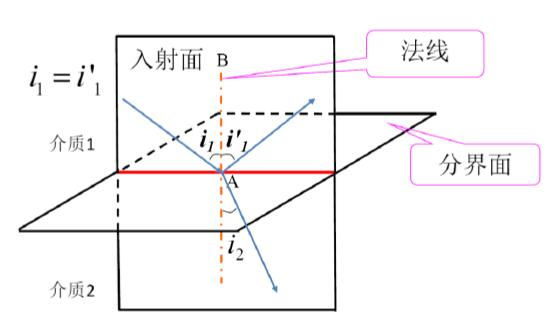
\includegraphics[height=120pt]{assets/1,2/image (44).jpg}
    \caption{ 反射与折射 }
\end{subfigure}\hfill
\begin{subfigure}[t]{0.5\columnwidth}\centering
    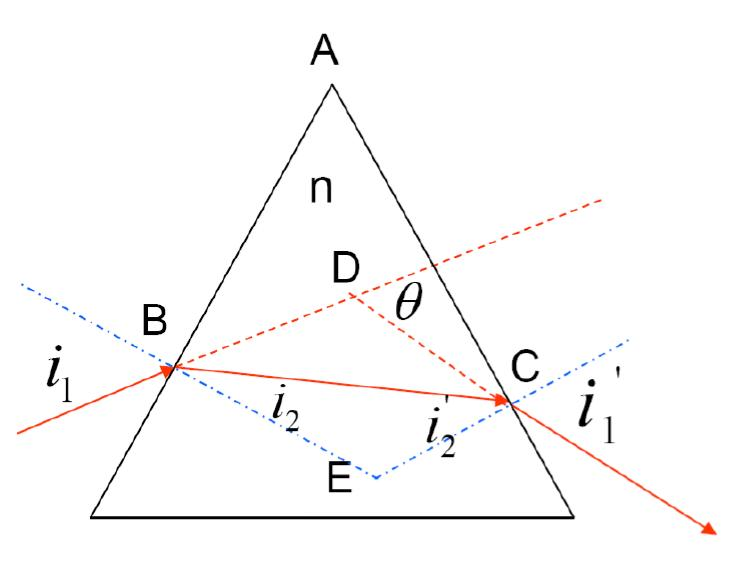
\includegraphics[height=120pt]{assets/1,2/image (45).jpg}
    \caption{ 三棱镜最小偏向角 }
\end{subfigure}
\caption{ 反射与折射、三棱镜最小偏向角 }\label{反射与折射、三棱镜最小偏向角}
\end{figure}



特别地,作为色散的一个例子,我们考虑三棱镜的最小偏向角。如图 \ref{反射与折射、三棱镜最小偏向角} (b) 所示,最小偏向角 $\theta_0 = (i_1 - i_1')_{\min}$ 满足:
\begin{equation}
    \theta_0 = 2i_1 - A, \quad \frac{n_2}{n_1} = \frac{\sin\frac{\theta_0+A}2}{\sin\frac A2}
\end{equation}



\section{惠更斯原理与费马原理}

\begin{LineTheorem}[惠更斯原理]\label{LineTheorem: 惠更斯原理}
    由振源发出的波动在 $t$ 时刻传播到一个波面 $S$,波面上的每一个面元可认为是次波的波源。由面元发出的次波向四面八方传播。在以后的时刻 $t'$ 形成次波面。这些次波面的包络面 $S'$ 就是 $t'$ 时刻总扰动的波面。
\end{LineTheorem}

\noindent 其中:
\begin{enumerate}
    \item 波面:在同一振源的波场中,扰动同时到达的各点具有相同的相位,这些点的轨迹构成一个曲面,称为波面(也称为等相位面)。
    \item 波线:与波面处处正交的曲线称为波线,其切线方向为光的传播方向
\end{enumerate}

\noindent 几何光学的定律需要前提条件:
\begin{enumerate}
\item 必须是均匀介质,即同一介质的折射率处处相等,折射率不是位置的函数。
\item 必须是各向同性介质,即光在介质中传播时各个方向的折射率相等,折射率不是方向的函数。
\item 光强不能太强,否则巨大的光能量会使线性叠加原理不再成立而出现非线性情况。
\item 光学元件的线度应比光的波长大得多,否则不能把光束简化为光线。
\end{enumerate}

\begin{figure}[H]\centering
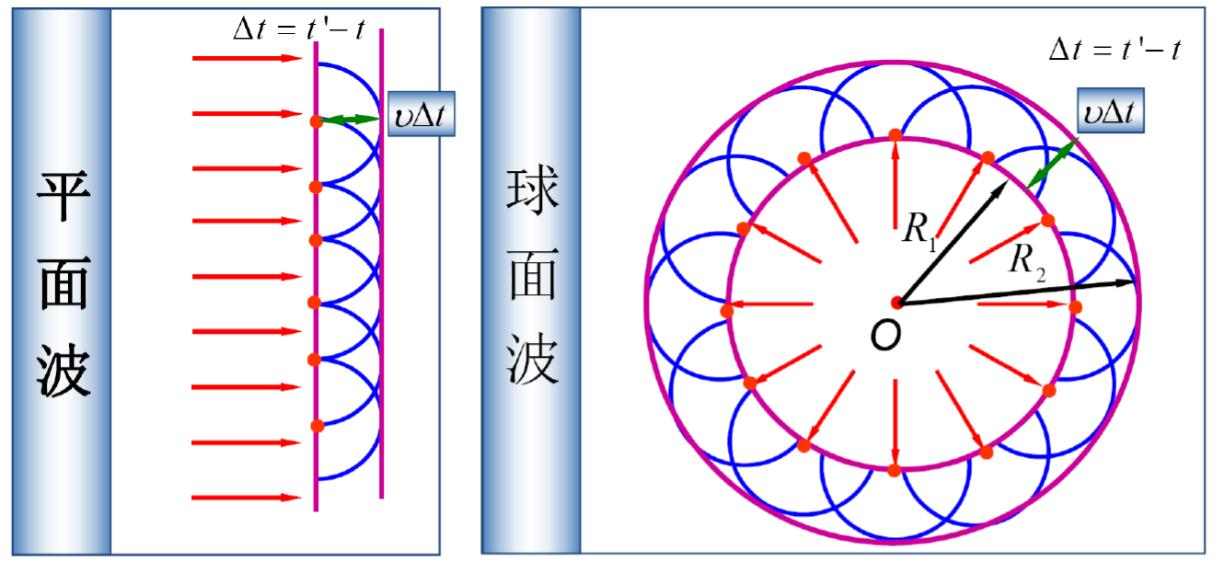
\includegraphics[width=0.5\textwidth]{assets/1,2/image (46).jpg}
\caption{惠更斯原理}\label{惠更斯原理}
\end{figure}

\begin{BlockTheorem}[费马原理]\label{费马原理}
光从空间中一点传播到另一点时,总是沿光程(Optical Length, OPL)平稳的路径传播\footnote{这里的平稳相当于“极值”,可以是极小值、极大值或常数,一般情况下,实际光程大多取极小值。极大值(如凹面镜成像)、拐点(如椭球面镜、凸透镜)的例子,可以参考 \href{https://zhuanlan.zhihu.com/p/107739173}{知乎:浅谈几何光学(1)——费马原理}}。写成公式即为:
\begin{equation}
    \mathrm{d}\ \mathrm{OPL} =  \mathrm{d}\left(\int_{Q}^{P} n \ \mathrm{d} l\right)=0 \Longrightarrow \frac{\mathrm{d}\  \mathrm{OPL} }{\mathrm{d} \varphi } = \frac{\mathrm{d} OPL }{\mathrm{d} s } = 0 
\end{equation}
\end{BlockTheorem}
由费马原理可以导出诸多推论,包括我们熟知的几条基本原理,还有物像之间的等光程性(例如凸透镜):
在物点Q与像点Q’之间,不管光线经何路径,凡是由Q通过同样的光学系统到达Q’的光线,都是等光程的。

\section{成像}

理想的像与物体在形状上一致,大小成比例。物与像之间的关系:本质上是一系列物点与像点的点点对应,推广至线线、面面对应。

同心光束:各光线本身或其延长线交于同一点的光束称为同心光束,在各向同性介质中,它对应于球面波。

由若干反射面或折射面组成的光学系统称为光具组。

\begin{enumerate}
\item 实物:发散的同心入射光束的“心”
\item 虚物:汇聚的同心入射光束的“心”
\item 实像:发散的同心出射光束的“心”
\item 虚像:汇聚的同心出射光束的“心”
\end{enumerate}

\subsection{物像的共轭性(可逆性)}

若 $P$ 为 物体 $P$(可实可虚)的像点,则反之,当物点为 $P$ 时,像点必在点 $P'$(实际光路可能不同)。是光路可逆性的必然结果。 

计算由物到像的 OPL 时,若为实线(实物、实像)则取正,称为实光程,若为虚线(虚物、虚像)则取负,称为虚光程。

\begin{figure}[H]\centering
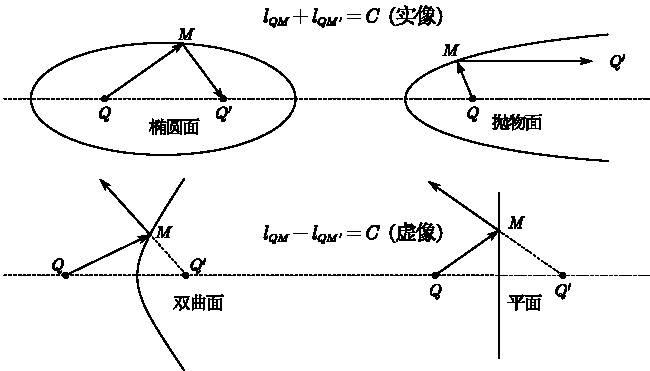
\includegraphics[width=0.6\textwidth]{assets/1,2/path2.pdf}
\caption{光程恒定的例子}\label{光程恒定的例子}
\end{figure}


\subsection{折射球面与反射球面}


的
对于折射球面,存在一对恰好成像的共轭点,称为齐明点。在齐明点处,可以证明 $Q$ 到 $Q'$ 的光程(即物像间的OPL)$l_{QQ'}$。

\begin{align}
\begin{matrix}
    \text{折射球面公式:}& \displaystyle \frac{n_1}{l_1} + \frac{n_2}{l_2} = \frac{1}{R\,}\left( \frac{n_{{\color{red} 2}}s_{{\color{red} 2}}}{l_{{\color{red} 2}}} - \frac{n_1s_1}{l_1} \right) & \displaystyle {\color{gray} \Longrightarrow     \frac{n'}{s'}  +  \frac{n}{s} = \frac{n'-n}{r}\quad  \text{(傍轴)}} 
    \vspace*{3pt}\\ 
    \text{反射球面公式:}& \displaystyle  \frac{1}{l_1} + \frac{1}{l_2} = {\color{red} -}\frac{2}{R\,}\left(\frac{s_1}{l_1} + \frac{s_2}{l_2}  \right) & \displaystyle {\color{gray} \Longrightarrow   \frac{1}{s} + \frac{1}{s'} = -\frac{2}{\,r\,} \quad  \text{(傍轴)}}
\end{matrix}
\end{align}



\begin{figure}[H]\centering
\begin{subfigure}[t]{0.45\textwidth}\centering
    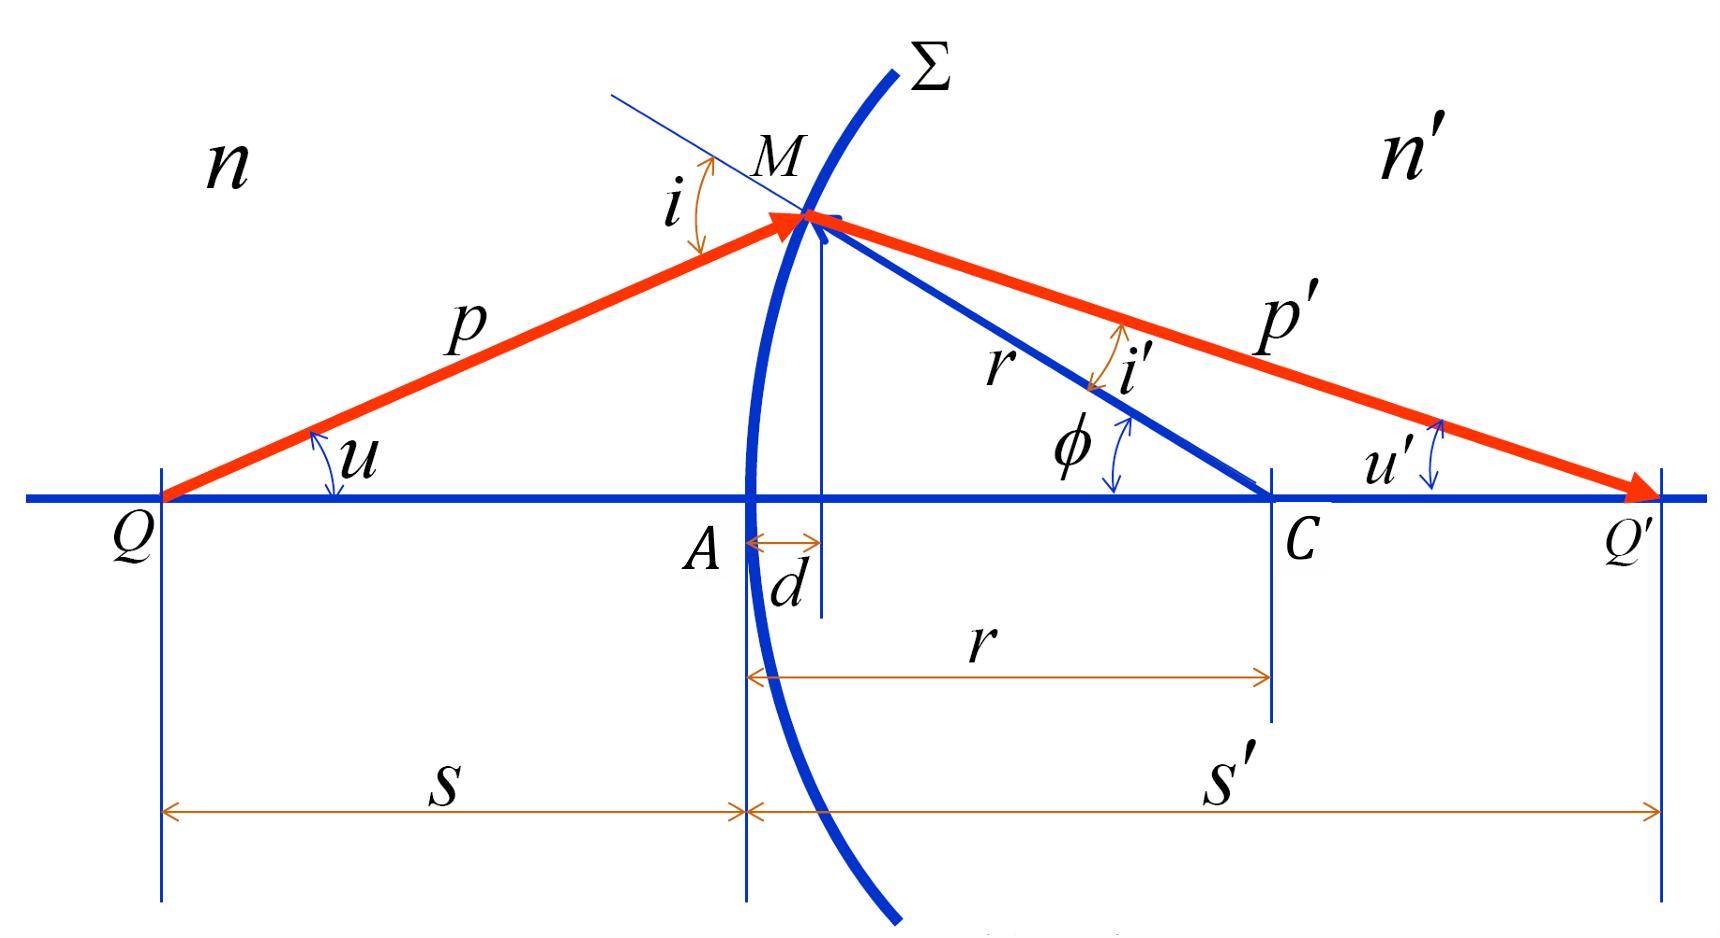
\includegraphics[height=100pt]{assets/1,2/image.jpg}
    \caption{ 折射球面 }
\end{subfigure}\begin{subfigure}[t]{0.4\textwidth}\centering
    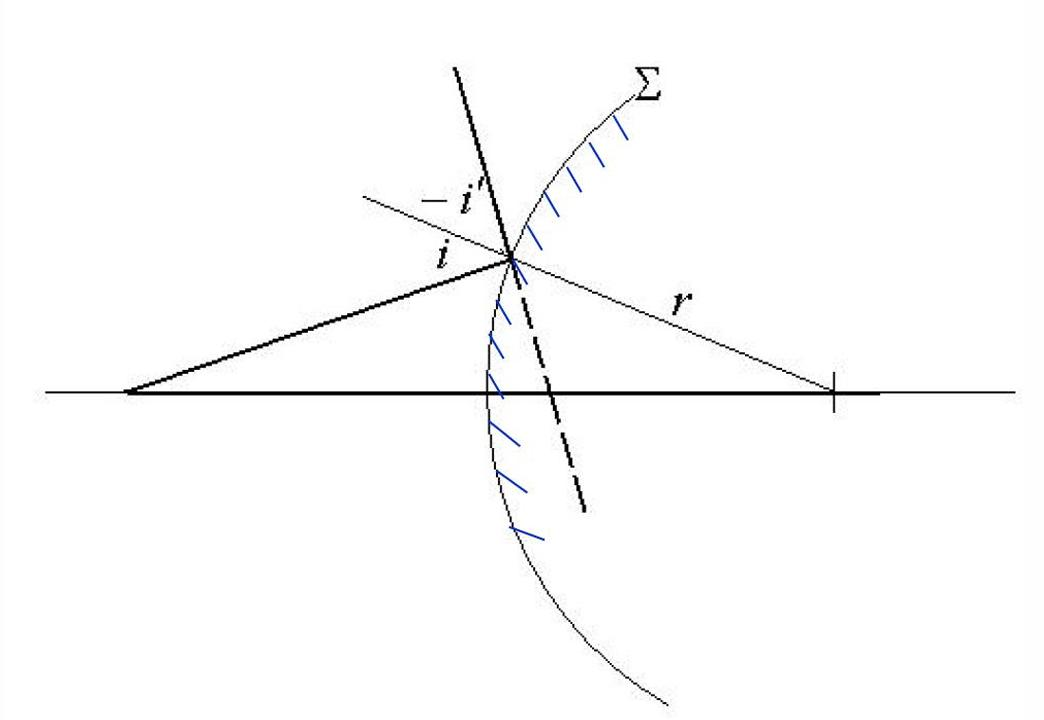
\includegraphics[height=100pt]{assets/1,2/image (1).jpg}
    \caption{ 反射球面 }
\end{subfigure}
\caption{ 折射球面与反射球面 }
\end{figure}


\subsection{像的放大率}


放大率公式:
\begin{equation}
\frac{n_1 | y_1 |}{s_1} = \frac{n_2 | y_2 |}{s_2}
\end{equation}

Lagrange-Helmholtz 恒等式:
\begin{equation}
n_1u_1y_1 = n_2u_2y_2
\end{equation}

上式的 $u$ 和 $y$ 是有正负的,例如折射球面中 $u_1 > 0,\ y_1 >0$ 而 $u_2 <0,\ y_2 < 0$。







\section{薄透镜}

透镜是由两个共轴折射球面构成的光具组,球面间距远远小于球面半径和物距像距的透镜称为薄透镜,也即 $d \ll | R_1 |, | R_2 |, | s |, | s' |$。此时可以认为两球面顶点重合,称为光心。

薄透镜成像公式(物像距公式):
\begin{gather} 
\frac{n}{s} + \frac{n'}{s'} = \frac{n_L - n}{r_1} + \frac{n' - n_L}{r_2} \label{薄透镜成像公式} \\
s' = \infty \Longrightarrow  f = \frac{n}{\frac{n_L - n}{r_1} + \frac{n' - n_L}{r_2}}\quad \text{物方焦距} \label{物方焦距} \\ 
s = \infty \Longrightarrow  f' = \frac{n'}{\frac{n_L - n}{r_1} + \frac{n' - n_L}{r_2}}\quad \text{像方焦距} \label{像方焦距}
\end{gather}
故物像焦距满足 $\frac{f}{n} = \frac{f'}{n'}$。
特别地,当物像方折射率都为 1 时(真空),我们有磨镜者公式和像的横向放大率:
\begin{equation}
f =f' = \frac{1}{(n_L - 1)(\frac{1}{r_1} - \frac{1}{r_2})},\quad  V = -\frac{\frac{s'}{n'}}{\frac{s}{n}} = -\frac{fs'}{f's} =  - \frac{s'}{s}
\end{equation}


将公式 \ref{物方焦距} 和公式 \ref{像方焦距} 代入式 \ref{薄透镜成像公式} 中,可以得到 Gauss 物像公式:
\begin{equation}
\frac{f}{s} + \frac{f'}{s'} = 1 \overset{n = n'}{\ \ \ \Longrightarrow\ \ \  } \frac{1}{s} + \frac{1}{s'} = \frac{1}{f}
\label{Gauss物像公式}
\end{equation}

令 $s = x + f$,$s' = x' + f'$,代入公式 \ref{Gauss物像公式},可以得到 Newton 物像公式:
\begin{equation}
xx = ff'
\end{equation}

\section{光度学基本概念}

在学习光度学之前,需要区分辐射度学与光度学中的基本概念。辐射度学研究的是辐射能量对实际物体的影响,而光度学研究的是辐射能量对人眼的影响,是基于人眼实验数据的学科,例如 Luminous Efficiency Function。它们的概念相互对应(可以相互转化)但并不相同,如下表所示: 
\begin{table}[H]\centering
    \caption{光度学与辐射度学概念对应关系}
    \label{光度学与辐射度学概念对应关系}
    \resizebox{\linewidth}{!}{   % 设置宽度为 \linewidth 等比例缩放
    \begin{tabular}{|c|c|c|c|c|c|c|c|}
        \hline
        学科范围 & \multicolumn{7}{c|}{基本概念} \\
        \hline
        辐射度学 & 辐射能 $Q_e$  & 辐射通量 $\Phi_e$  & 辐射强度 $I_e$ & 辐射亮度 $L_e$ &  辐射照度 $E_e$ & 辐射出射度 $M_e$ & 辐射通量谱密度 $\Phi_{e,\lambda}$ \\
        \hline
        光度学   & 光量 $Q_v$ &  光通量 $\Phi_v$  & 光强度 $I_v$ & 光亮度 $L_v$ & 光照度 $E_v$ & 光出射度 $M_v$ & 光通量谱密度 $\Phi_{v,\lambda}$\\
        \hline
    \end{tabular}
    }
\end{table}



\subsection{辐射度学基本概念}
下表展示了辐射度学的一些基本概念:
\begin{table}[H]\centering
    \caption{辐射度学基本概念}
    \label{辐射度学基本概念}
    \renewcommand{\arraystretch}{1.1} % 调整行间距为默认值的1.5倍
%\resizebox{0.9\linewidth}{!}{   % 设置宽度为 \linewidth 等比例缩放
%}
\begin{tabular}{|c|c|c|c|c|c|c|c|c|c|}\hline
    名称 & 符号& 定义式 & 单位 & 概念描述\\
    \hline
    辐射能 & $Q_e$ & - & J & 以辐射形式传播的能量 \\
    \hline
    辐通量 & $\Phi_e$ & $\Phi_e = \frac{\mathrm{d}Q_e}{\mathrm{d}t}$ & W & 单位时间内流过某截面的辐射能量 \\
    \hline
    辐强度 & $\boldsymbol{I}_e$ & $\boldsymbol{I}_e = \frac{\mathrm{d}\Phi_e }{\mathrm{d} \boldsymbol{\Omega} } $ & $\mathrm{W\cdot sr^{-1}}$ & 点辐射源在某方向上单位立体角\footnote{立体角的定义参考 \href{https://www.zhihu.com/question/611533175/answer/3244345528}{辐亮度和辐照度是如何计算的}}内的辐射通量 \\
    \hline
    辐照度 & $\boldsymbol{E}_e$ & $ \boldsymbol{E}_e = \frac{\mathrm{d}\Phi_e}{\mathrm{d}\boldsymbol{A}}$ & $\mathrm{W\cdot m^{-2}}$ & 被辐射体单位面积上的辐射通量 \\
    \hline
    辐亮度 & $\boldsymbol{L}_e$ & $\boldsymbol{L}_e = \frac{\mathrm{d}\boldsymbol{I}_e}{\mathrm{d}A \cos \theta} $ & $\mathrm{\mathrm{W}\cdot sr^{-1}\cdot m^{-2}}$ & 单位面积的面辐射源在某方向上的辐射强度\\
    \hline
    辐出射度 & $M_e$ & $ M_e = \frac{\mathrm{d}\Phi_e}{\mathrm{d}A}$ & $\mathrm{W\cdot m^{-2}} $ & 辐射体单位面积向半球空间发射的辐射通量 \\
    \hline
    辐谱密度 & $\phi_e$ & $\phi_e = \frac{\Delta \Phi_{e,\lambda}}{ \Delta\lambda} $ & $\mathrm{W\cdot m^{-1}} $ & 辐射能(通量)在频谱中的分布 \\
    \hline
\end{tabular}
\end{table}

其中 $\Delta \Phi_{e,\lambda}$ 表示波长为 $\lambda$(也可认为是 $[\lambda,\ \lambda + \Delta \lambda]$)的部分所贡献的辐射通量。

\subsection{明视觉曲线}

人眼对不同波长的光具有不同的明亮感觉程度\footnote{参考 \href{https://www.writebug.com/static/uploads/2024/9/16/09153f4fce1d2b99e38c19ef9deeda44.pdf}{新旧明视觉光谱光视效率曲线.pdf}。},称为明视觉光谱光视效率曲线\footnote{参考 \href{https://webstore.ansi.org/preview-pages/ESTA/preview_E1-48_2014.pdf}{ANSI E1.48 - 2014 (A Recommended Luminous Efficiency Function for Stage and Studio Luminaire Photometry)},国际照明委员会(CIE)规定的标准光谱光视效率函数 \href{https://rdrr.io/cran/colorSpec/man/luminsivity.html}{Luminous Efficiency Functions} 或者 \href{https://www.zhihu.com/question/400643965/answer/2727547334}{知乎:光通量与光辐照度之间的换算}。}(函数),常简称为“明视觉曲线”或“视觉曲线”,记为 $V = V(\lambda)$。

光谱光效能 $K$,表示在某一波长上每一瓦辐射通量可以产生多少流明的光通量。光谱光视效率 $V = V(\lambda)$,就是归一化的光谱光效能:
\begin{equation}\label{光谱光效能}
    K = \frac{\Delta \Phi_{v,\lambda}}{\Delta \Phi_{e,\lambda}} = \frac{\phi_v(\lambda)}{\phi_e(\lambda)}, \quad V(\lambda) = \frac{K(\lambda)}{K_{\text{max}}} = \frac{1}{K_{\text{max}}}\cdot \frac{\phi_v(\lambda)}{\phi_e(\lambda)}
\end{equation}
$K_{\text{max}} = 683\ \mathrm{lm \cdot W^{-1}}$ 在波长约 555.0 nm 取到,因此 $V = V(\lambda)$ 也表示在相同辐射通量下,波长为 $\lambda$ 的光与 555.0 nm 的光所产生的亮暗感觉比值。

另外,公式 \ref{光谱光效能} 建立了辐射度学参量与光度学参量之间的转化关系:
\begin{equation}
\Phi_v(\lambda) 
= \int \phi_v(\lambda) \mathrm{d} \lambda 
= \int K_{\text{max}}V(\lambda)\phi_e(\lambda) \mathrm{d} \lambda  
\end{equation}

\subsection{光度学基本概念}\label{光度学基本概念}
表 \ref{光度学基本概念表} 展示了光度学的一些基本概念,它们\footnote{参考 \href{https://www.zhihu.com/question/53080536/answer/133398317}{知乎:如何区分并记忆光度、照度、发光强度、光强、亮度等}}之间的转化关系:
\begin{gather}
\text{与光通量的转换:} \Phi_v = \int \boldsymbol{E}_v \mathrm{d}\boldsymbol{A} = \int \boldsymbol{I}_v \mathrm{d}\boldsymbol{\Omega} = \iint \boldsymbol{L}_v \cos \theta\, \mathrm{d}A \,\mathrm{d} \boldsymbol{\Omega} \\ 
\text{与光强的转换:} \boldsymbol{I}_v = r^2\boldsymbol{E}_v = \int \boldsymbol{L}_v \cos \theta\, \mathrm{d}A = \int \boldsymbol{L}_v  \mathrm{d}A_{\perp}
\end{gather}

计算时的常用微分:
\begin{gather}
\begin{aligned}
    & \text{直角坐标系:}&& \mathrm{d}A = \mathrm{d}x \mathrm{d}y &&,  \mathrm{d}\boldsymbol{\Omega} = \frac{\mathrm{d}\boldsymbol{A}}{r^2} \\ 
    & \text{球坐标系:}&& \mathrm{d}A = r^2 \sin \theta \mathrm{d}\theta \mathrm{d}\phi &&,\mathrm{d}\Omega = \sin \theta \mathrm{d}\theta \mathrm{d}\phi \\ 
\end{aligned}
\end{gather}
\begin{table}[H]\centering
    \caption{光度学基本概念}\label{光度学基本概念表}
    \renewcommand{\arraystretch}{1.15} % 调整行间距为默认值的1.5倍
%\resizebox{0.9\linewidth}{!}{   % 设置宽度为 \linewidth 等比例缩放
%}
\begin{tabular}{|c|c|c|c|c|c|c|c|c|c|}\hline
    名称 & 符号& 定义式 & 单位 & 概念描述\\
    \hline
    光量 & $Q_v$ & $Q_v(\lambda) = V(\lambda)\cdot Q_e(\lambda)$ & $\mathrm{cd \cdot sr \cdot s}$ & 辐射能的光度量大小 \\
    \hline
    光通量 & $\Phi_v$ & $\Phi_v = \frac{\mathrm{d}Q_v}{\mathrm{d}t}$ & $\mathrm{lm} = \mathrm{cd \cdot sr}$ & 单位时间内流过某截面的光度学光量 \\
    \hline
    光强度 & $\boldsymbol{I}_v$ & $\boldsymbol{I}_v = \frac{\mathrm{d}\Phi_v }{\mathrm{d} \boldsymbol{\Omega} } $ & $\mathrm{cd}$ & 点辐射源在某方向上单位立体角内的光通量 \\
    \hline
    光照度 & $\boldsymbol{E}_v$ & $ \boldsymbol{E}_v = \frac{\mathrm{d}\Phi_v}{\mathrm{d}\boldsymbol{A}}$ & $\mathrm{lm \cdot m^{-2}}$ & 被辐射体单位面积上的光通量 \\
    \hline
    光亮度 & $\boldsymbol{L}_v$ & $\boldsymbol{L}_v = \frac{\mathrm{d}\boldsymbol{I}_v}{\mathrm{d}A \cos \theta} $ & $\mathrm{cd \cdot m^{-2}}$ & 单位面积的面辐射源在某方向上的光强度 \\
    \hline
    光出射度 & $M_v$ & $ M_v = \frac{\mathrm{d}\Phi_v}{\mathrm{d}A}$ & $\mathrm{lm \cdot m^{-2}} $ & 辐射体单位面积向半球空间发射的光通量 \\
    \hline
    光谱密度 & $\phi_v$ & $\phi_v = \frac{\Delta \Phi_{v,\lambda}}{ \Delta\lambda} $ & $\mathrm{lm \cdot m^{-1}}$ & 光量(光通量)在频谱中的分布 \\
    \hline
\end{tabular}
\end{table}

\section{特殊发光体(略)}

\section{章末总结}

\begin{align}
&
\text{电磁波的四个恒等式:} \begin{cases}
    nv = c \\ 
    \varepsilon \mu v^2 = 1 \\ 
    \varepsilon_r \mu_r = n^2 \\ 
    E = vB
\end{cases} 
\\ &
\text{波印廷与辐照度:} \begin{cases}
    S = | \boldsymbol{E}\times \boldsymbol{H} | = \varepsilon w = \varepsilon v E^2 \\ 
    I = \langle  S  \rangle_T \overset{\text{简谐}}{=} \frac{1}{2}\varepsilon v E^2 
\end{cases}
\\ &
\text{光压 (吸收) : \ } pc = I = \langle S \rangle \overset{\text{简谐}}{\Longrightarrow} p = \frac{\varepsilon v E^2}{2c}
\\ &
\text{惠更斯原理:} \ \text{波阵面上每一点都是次波源,次波面的包络面是新波阵面}
\\ &
\text{费马原理:} \ \text{光沿光程平稳的路径传播,即光程取极值}
\\ &
\text{三棱镜最小偏向角:} n = \frac{\sin \left(\frac{\alpha + \delta}{2}\right)}{\sin \left(\frac{\alpha}{2}\right)} 
\\ &
\text{发光体:}
\begin{cases}
    \text{点光源照度 $E$ :\ }E = \frac{\cos \theta}{r^2}\cdot I \\ 
    \text{半球面亮度 $B$ 与照度 $E$ :\ } E = \pi B
\end{cases} 
\\ &
\text{光路方程:}
\begin{cases}
    \text{一维:} y'' = \frac{1}{2n_0^2\cos^2 \theta_0}\cdot \frac{\mathrm{d} n^2 }{\mathrm{d} y } = A\cdot \frac{\mathrm{d} A }{\mathrm{d} y },\quad A = \frac{n}{n_0\cos \theta_0} \\ 
    \text{三维:} \nabla n = \frac{\mathrm{d}  }{\mathrm{d} s }\left(n\, \frac{\mathrm{d} \boldsymbol{r} }{\mathrm{d} s }\right)
\end{cases}
\\ &
\text{球面焦距:}
\begin{cases}
    \text{折射球面:}\begin{cases}
        f = n \cdot \frac{r}{n' - n} \\ 
        f' = n' \cdot \frac{r}{n' - n}
    \end{cases} \\ 
    \text{反射球面:}f = f' = - \frac{r}{2}
\end{cases}
\\ &
\text{薄透镜:}
\begin{cases}
    f = n \cdot \frac{1}{\frac{n_L - n}{r} - \frac{n_L - n'}{r'}} \\ 
    f' = n' \cdot \frac{1}{\frac{n_L - n}{r} - \frac{n_L - n'}{r'}}
    \text{磨镜者公式 ($n = n' = 1$) : }f = f' = \frac{1}{\left(n_L - 1\right)\left(\frac{1}{r} - \frac{1}{r'}\right)}
\end{cases}
\\ &
\text{成像公式:}
\begin{cases}
    \text{Gauss 公式:} \frac{f}{s} + \frac{f'}{s'} = 1 \\ 
    \text{Newton 公式:} xx' = ff'\\
    \text{亥姆霍兹公式:} yn \tan u = y'n' \tan u'\\
    \text{横向放大率:} \frac{ny}{s} + \frac{n'y'}{s'} = 0 \Longrightarrow V = \frac{y'}{y} =  - \frac{ns'}{n's}=  - \frac{fs'}{f's}\\
    \text{角放大率:} W = \frac{\tan u'}{\tan u},\quad VW = \frac{f}{f'}\\
    \text{密接透镜组:} \frac{1}{f} = \sum \frac{1}{f_i}
\end{cases}
\end{align}



\chapter{光的反射与折射}\thispagestyle{fancy}

在本章,我们先以一定的顺序,依次对反射折射过程中所出现的现象或相关物理量进行讨论,最后给出所有现象的总结。

\section{菲涅尔公式}

\begin{BlockTheorem}[菲涅尔公式, Fresnel Formula]\label{菲涅尔公式}
光线在通过两介质分界面时通常会同时发生折射(透射)和反射现象,设入射光(incident ray)介质折射率 $\eta_i$,入射角 $\theta_i$,透射光(transmitted ray)介质折射率 $\eta_t$,透射角(折射角)$\theta_t$,则有\footnote{对于金属材质(非绝缘材质),需要引入消光系数 $k_t$ 来修正菲涅尔公式(绝缘材质等价于 $k_t = 0$),具体参见 \href{https://zhuanlan.zhihu.com/p/480405520?utm_psn=1818236176659771392}{知乎: 菲涅尔公式}}:

%\lstinputlisting[language=matlab]{D:/a_RemoteRepo/GH.MatlabCodes/本科课程代码/光学/a3.m}

%\begin{matlablisting}
%    disp(['Y_bar = ', num2str(stc_error.Y_bar, '%.8f')]); disp(['Y_bar = ', num2str(stc_error.Y_bar, '%.8f')]); disp(['Y_bar = ', num2str(stc_error.Y_bar, '%.8f')]); disp(['Y_bar = ', num2str(stc_error.Y_bar, '%.8f')]); 
%\end{matlablisting}


\begin{table}[H]
\centering
\renewcommand{\arraystretch}{1.6} % 调整行间距为默认值的1.5倍 
\begin{tabular}{|c|c|c|c|c|} 
\hline
类型 & \multicolumn{2}{c|}{振幅反射系数 $r$} & \multicolumn{2}{c|}{振幅透射系数 $t$ }  \\ 
\hline
$s$ 波 & $\displaystyle r_s = \frac{n_{{\color{red} i}}\cos \theta_{{\color{red} i}} - n_t \cos \theta_t}{n_{{\color{red} i}}\cos \theta_{{\color{red} i}} + n_t \cos \theta_t} $ & $\displaystyle  - \frac{\sin (\theta_i - \theta_t) }{\sin (\theta_i + \theta_t)}$ & $\displaystyle t_s  = \frac{2n_{{\color{red} i}} \cos \theta_{{\color{red} i}}}{n_{{\color{red} i}}\cos \theta_{{\color{red} i}} + n_t \cos \theta_t} $ &   $\displaystyle   \frac{2 \sin \theta_t \cos \theta_i}{\sin (\theta_i + \theta_t)}$   \\ 
\hline
$p$ 波 & $\displaystyle r_p = \frac{n_t\cos \theta_{{\color{red} i}} - n_{{\color{red} i}} \cos \theta_t}{n_t\cos \theta_{{\color{red} i}} + n_{{\color{red} i}} \cos \theta_t} $ &     $ \displaystyle  + \frac{\tan (\theta_i - \theta_t)}{\tan (\theta_i + \theta_t)} $  &  $\displaystyle t_p  = \frac{2n_{{\color{red} i}} \cos \theta_{{\color{red} i}}}{n_{{\color{red} i}}\cos \theta_t + n_t \cos \theta_{{\color{red} i}}} $ &   $\displaystyle \frac{2 \sin \theta_t \cos \theta_i}{\sin (\theta_i + \theta_t) \cos (\theta_i - \theta_t)}$                  \\
\hline
\end{tabular}
\end{table}

注意,$t_p$ 分子上的两个角标都是 $i$,这意味着有 $(-r_s) + t_s = 1$,但并没有 $r_p + t_p = 1$,而应该是:
\begin{equation}
    r_p + \frac{\cos \theta_t}{\cos \theta_i}\cdot t_p = 1
\end{equation}

折射角 $\theta_t$、$s$ 波通量反射率 $R_s$、$p$ 波通量反射率 $R_p$ 和总通量反射率 $R$ 为:
\begin{equation}
    \cos \theta_t = \sqrt{1 - \left( \frac{n_i}{n_t} \sin \theta_i\right)^2},\quad R_s = r_s^2,\ R_p = r_p^2, \quad  R = \frac{1}{2}\left( R_s + R_p \right)
\end{equation}

总强度反射率 $R$ 的严格证明见下一节。特别地,若 $1 - \left( \frac{n_i}{n_t} \sin \theta_i\right)^2 < 0$,则发生全反射,此时 $R = 1$。另外,需要指出菲涅尔公式的适用条件,也即推导时所做的一些假设,如下:
\begin{enumerate}
\item 介质为绝缘介质,无表面自由电荷或传导电流
\item 介质为各向同性的光学线性介质(弱光强)
\item 介质磁导率(约)等于真空磁导率\footnote{对于介质磁导率不等于真空磁导率的情况,详见参考文献 \cite{Optics} Page 144} $\mu_i = \mu_t = \mu_0$,其中 $\mu_0$ 为真空磁导率。
\end{enumerate}
\end{BlockTheorem}

\section{反射时的相位变化}

菲涅尔公式的推导以矢量分析为基础,因此公式中系数 $r_s$ 的正负具有明确物理意义,它标识着方向。若为负,则反射后的方向与原方向相反,否则相同。各系数正负情况见表 \ref{振幅系数的正负情况},其中 o 表示可正可负。

%\footnote{拓展阅读 \href{https://zhuanlan.zhihu.com/p/607510257}{知乎:你一直没搞懂的半波损失(机械波、光波)}}

\begin{center}\noindent\begin{minipage}{0.65\columnwidth}
    \hspace*{2em} 从波的角度,方向相反可以等价地视为相位发生了 $\pi$ 的前移(或后移),称为相位突变。$n_i < n_t$ 时,相位突变要么是 0,要么是 $\pi$,$n_i > n_t$ 时的相位变化比较复杂,我们不深究。在 $\theta_i + \theta_t = \frac{\pi}{2}$ 时,$r_p$ 的正负发生变化,$p$ 波的反射波相位也发生突变,称此时 $\theta_i$ 的角度为布儒斯特角(Brewster angle),记为 $\theta_B$,也称为偏振角或起偏角。
\end{minipage}\hfill\begin{minipage}{0.3\columnwidth}
    \begin{table}[H]\centering
        % \setlength{\tabcolsep}{1.5mm} % 调整列间距
            \caption{\textbf{振幅系数的正负情况}}
            \label{振幅系数的正负情况}
        \begin{tabular}{cccccccccc}\toprule
            折射率 & $r_s$& $r_p$ & $t_s$ & $t_p$\\
            \midrule                        
            $n_i < n_t$ & $-$ & o & $+$ & $+$\\
            $n_i > n_t$ & o & o & $+$ & $+$\\
            \bottomrule
        \end{tabular}
    \end{table}
\end{minipage}\end{center}

\begin{figure}[H]\centering
\begin{subfigure}[t]{0.49\textwidth}\centering
    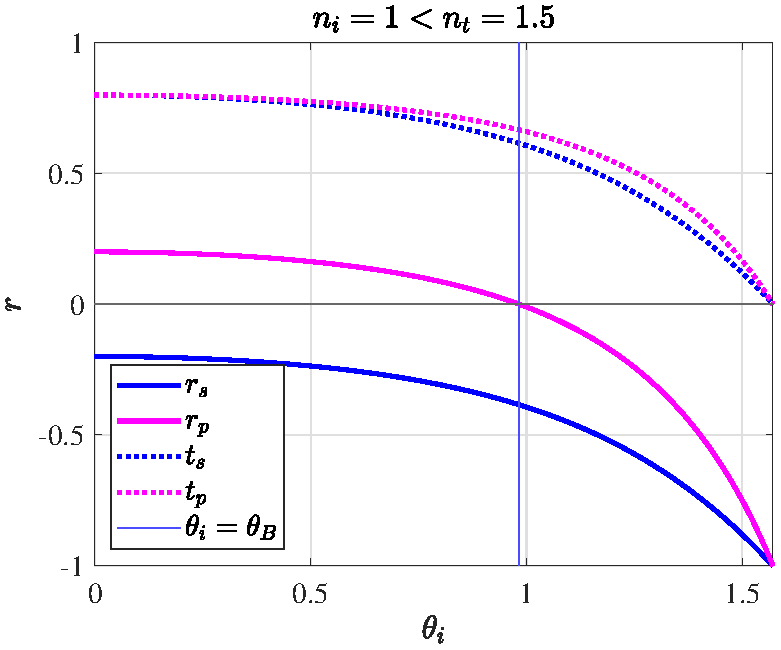
\includegraphics[height=190pt]{assets/1,2/2024-09-15_10-53-31.pdf}
    \caption{ 由空气入射玻璃 ($n_i = 1,\ n_t = 1.5$) }
\end{subfigure}
\begin{subfigure}[t]{0.49\textwidth}\centering
    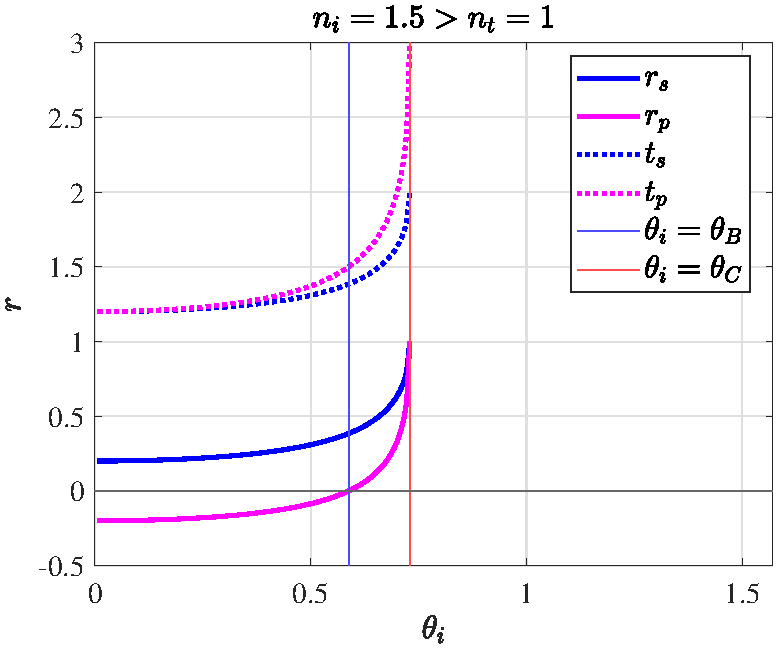
\includegraphics[height=190pt]{assets/1,2/2024-09-15_10-53-27.pdf}
    \caption{ 由玻璃入射空气 ($n_i = 1.5,\ n_t = 1$) }
\end{subfigure}
\caption{ 振幅系数 $r$ 随入射角 $\theta_i$ 的变化 }\label{振幅系数随入射角的变化}
\end{figure}

\begin{figure}[ht]\centering
    \includesvg[width=0.93\textwidth]{assets/1,2/相位突变.svg}
    \caption{ $s$ 波和 $p$ 波在反射时的相位变化}\label{反射时 s 波和 p 波的相位变化}
\end{figure}

\begin{figure}[H]\centering
\includesvg[width=0.95\textwidth]{assets/1,2/反射后的方向情况.svg}
\caption{ 由空气入射玻璃的光线示意图}\label{反射示意图}
\end{figure}

可以推得 Brewster angle 的值为:
\begin{equation}
    \theta_B = \arctan \left( \frac{n_2}{n_1} \right)
\end{equation}


具体的振幅系数变化见图 \ref{振幅系数随入射角的变化}\footnote{源码见附录 \ref{振幅系数随入射角的变化 源码}},相位增量见图 \ref{反射时 s 波和 p 波的相位变化},反射示意图见图 \ref{反射示意图}。


由菲涅尔公式,当 $n_i < n_t$ 时,我们还有如下结论:
\begin{gather}
    \begin{aligned}
        &\text{$\theta_i = 0$ 时:} &&r_p = (-r_s)  = \frac{n_t - n_i}{n_t + n_i}, &&t_p = t_s = \frac{2n_i}{n_i + n_t} \\ 
        &\text{$\theta_i = \frac{\pi}{2}$ 时:} &&r_p = r_s  = -1,&&t_p = t_s  =0
    \end{aligned}
\end{gather}
这表明,即使是正射(垂直于介质分界面的入射,$\theta_i = 0$),一般也存在部分反射光。总之,当 $n_i < n_t$ 时,入射光的 s 分量在反射中一定会相位跃变,p 分量都有可能。

另外,菲涅尔公式还可写成:
\begin{gather}
\boxed{
\begin{aligned}
    &\quad\quad \quad \quad   (-r_s) + t_s  = 1, &&\quad 
    \quad \quad\quad   r_p + t_p = 1 
    \\ 
    &r_s = \frac{\cos \theta_i - \sqrt{n_{ti}^2 - \sin^2 \theta_i} }{\cos \theta_i + \sqrt{n_{ti}^2 - \sin^2 \theta_i}}, && r_p = \frac{n_{ti}^2\cos \theta_i - \sqrt{n_{ti}^2 - \sin^2 \theta_i} }{n_{ti}^2\cos \theta_i + \sqrt{n_{ti}^2 - \sin^2 \theta_i}}
\end{aligned}
}
\end{gather}

\section{完全偏振反射光}

当光波由布儒斯特角 $\theta_B$ 入射时,由 Fresnel Formula,$r_p = \frac{\tan (\theta_i - \theta_t)}{\tan (\theta_i + \theta_t)} = 0$,也即反射光的 p 分量为 0,仅存在 s 分量。这说明反射光是完全偏振光,$\boldsymbol{E}$ 的方向(称为振动方向)垂直于入射面。
{\par\color{gray}\small
但此时反射光能量占比 $F$ 很小\footnote{可以使用玻璃片堆得到强度较大的偏振光},例如,空气($n=1$)入射玻璃($n = 1.5$)时,$\theta_B = 56.310^\circ$,$F =0.0740 $;玻璃入射空气时,$\theta_B = 33.690^\circ$,$F =0.0740 $。
\par}

    % \begin{matlablisting}
    % n_i = 1;
    % n_t = 1.5;
    % 
    % theta_B = atan(n_t/n_i);
    % theta_t = @(theta_i) asin(n_i/n_t*sin(theta_i));
    % r_s = @(theta_i, theta_t) - sin(theta_i - theta_t)./sin(theta_i + theta_t);
    % r_p = @(theta_i, theta_t) + tan(theta_i - theta_t)./tan(theta_i + theta_t);
    % F = @(theta_i, theta_t) 0.5*( r_s(theta_i, theta_t)^2 + r_p(theta_i, theta_t)^2 );
    % 
    % theta_i = theta_B;
    % disp(['theta_B = ', num2str(rad2deg(theta_B))])
    % disp(['F = ', num2str(F(theta_i, theta_t(theta_i)))])
    % 
    % %{ 
    % Output:
    % theta_B = 56.3099
    % F = 0.073964
    % %}
    % \end{matlablisting}


\section{反射折射时的能量关系}

在 Fresnel Formula 中可以发现,$r_s^2 + t_s^2 \ne 1$,$r_p^2 + t_p^2 \ne 1$,是能量不守恒了吗?显然不是。那么,反射光和透射光的能量关系是怎样的?这需要借助辐射度学的相关概念。

如图,圆形光束从空气入射到分界面上的一个面元 $\boldsymbol{A}$(界面下是玻璃),以此面元为研究对象。考虑玻印亭矢量 $\boldsymbol{S} = \boldsymbol{E} \times \boldsymbol{B}$,即单位时间内通过单位面积的电磁辐射能量(单位面积辐射功率),于是瞬时辐射照度 $\boldsymbol{E}_e$: 
\begin{equation}
\boldsymbol{E}_e = \boldsymbol{S} = c^2 \varepsilon_0 \boldsymbol{E} \times \boldsymbol{B},\quad  E_e = \varepsilon_0 cE^2 \cdot \sqrt{\frac{\varepsilon_r}{\mu_r}} = \frac{\varepsilon_0 c}{\mu_r}\cdot  nE^2
\end{equation}
其中 $\varepsilon_r$,$\mu_r$ 分别为相对介电常量、相对磁导率,对空气近似有 $\varepsilon_r = \mu_r = 1$,于是

核心思想是 $\mathrm{d} Q_e = (\boldsymbol{E}_e \cdot \boldsymbol{A})\, \mathrm{d}t $。入射、反射、透射光束的截面面积分别为 $A \cos \theta_i,\ A \cos \theta_r,\ A \cos \theta_t$,设其瞬时辐射照度分别为$\boldsymbol{E}_i,\ \boldsymbol{E}_r,\ \boldsymbol{E}_t$ ,则辐射通量为:
\begin{equation}
\Phi_{e, k} = E_{e, k} A \cos \theta_k = \frac{\varepsilon_0 cA }{\mu_r}\cdot  n_k\cos \theta_k\,E_k^2,\quad  k = i, r, t
\end{equation}

分别写出入射、反射、透射光的辐射通量:
\begin{align}
\Phi_{e,i} &= \frac{\varepsilon_0 cA }{\mu_r} \cdot  n_i\cos \theta_i\,E_i^2 
= \frac{\varepsilon_0 cA }{\mu_r} \cdot  n_i\cos \theta_i\, \left( E_{i,s}^2 + E_{i,p}^2 \right) 
\\ 
\Phi_{e,r} 
&= \frac{\varepsilon_0 cA }{\mu_r} \cdot  n_i\cos \theta_i\,E_r^2 
= \frac{\varepsilon_0 cA }{\mu_r} \cdot  n_i\cos \theta_i\, \left( r_s^2E_{i,s}^2 + r_p^2E_{i,p}^2 \right) 
\\ 
\Phi_{e,t} 
&= \frac{\varepsilon_0 cA }{\mu_r} \cdot  n_t\cos \theta_t\,E_t^2 
= \frac{\varepsilon_0 cA }{\mu_r} \cdot  n_t \cos \theta_t \, \left( t_s^2E_{i,s}^2 + t_p^2E_{i,p}^2 \right) 
\end{align}

由于入射光可分解为 $s$ 波与 $p$ 波,我们自然想到它们俩在入射前后应该是能量守恒的,这指导我们分别作数学上的处理。对 $s$ 波,由菲涅尔定律(这说明已经做了近似 $\mu_r = 1$),做减法得到:
\begin{align*}
&n_i \cos \theta_i E_{i,s}^2 - n_i \cos \theta_i r_{i,s}^2E_{i,s}^2 -   n_t \cos \theta_t t_s^2E_{i,s}^2 \\
&= E_{i,s}^2 \left[ n_i\cos \theta_i \left( 1 - \frac{(n_i\cos \theta_i - n_t \cos \theta_t)^2}{(n_i\cos \theta_i + n_t \cos \theta_t)^2} \right) - n_t \cos \theta_t \cdot \frac{(2n_i \cos \theta_i)^2}{(n_i\cos \theta_i + n_t \cos \theta_t)^2} \right] \\ 
& = \frac{E_{i,s}^2}{(n_i\cos \theta_i + n_t \cos \theta_t)^2} \left[ n_i \cos \theta_i \cdot (4 n_i\cos \theta_i \cdot n_t \cos \theta_t) - 4 n_t \cos \theta_t \cdot n_i^2 \cos^2 \theta_i\right] \\ 
& = 0
\end{align*}

同理,考虑 p 分量,作减法可得到:
\begin{equation}
n_i \cos \theta_i E_{i,p}^2 - n_i \cos \theta_i r_{i,p}^2E_{i,p}^2 -   n_t \cos \theta_t t_p^2E_{i,p}^2 = 0
\end{equation}

代入即得:
\begin{equation}
    \Phi_{e,i} - \Phi_{e,r} - \Phi_{e,t} = 0 \Longrightarrow  \Phi_{e,i} = \Phi_{e,r} + \Phi_{e,t}
\end{equation}
这便验证了入射前后的能量是守恒的。

由此,我们可以定义一些能量系数:
\begin{gather}
\begin{aligned}
    &\text{强度反射率 $R$: }\ &&R = \frac{1}{2}(R_s + R_p), &&R_s = r_s^2, && R_p = r_p^2 \\
    &\text{强度透射率 $T$: }\ &&T = \frac{1}{2}(T_s + T_p), &&T_s =\frac{n_t \cos \theta_t}{n_i \cos \theta_i} \cdot  t_s^2, && T_p =\frac{n_t \cos \theta_t}{n_i \cos \theta_i} \cdot  t_p^2 \\
\end{aligned}
\end{gather}

这样,它们具有下面的性质,方便我们计算能量关系:
\begin{gather}
\boxed{
\begin{aligned}
    &R_s + T_s = 1, &&\quad  R_p + T_p = 1,&&\ \  R + T = 1 \\ 
    &\Phi_{e,r} = R\Phi_{e,i}, && 
    \Phi_{e,r,s} = R_s\Phi_{e,i,s}, &&  \Phi_{e,r,p} = R_p\Phi_{e,i,s} 
    \\ 
    &\Phi_{e,t} = T\Phi_{e,i}, && \Phi_{e,t,s} = T_s\Phi_{e,i,s}, && \Phi_{e,t,p} = T_p\Phi_{e,i,s}
\end{aligned}
}
\end{gather}

%{\color{red} todo 其中 $\Phi_{e,r} = R\Phi_{e,i}$ 和 $\Phi_{e,t} = T\Phi_{e,i}$ 是怎么来的?}




\section{全反射时的隐失波与穿透深度}

假设现在由光密介质射向光疏介质,即 $n_i > n_t$,则有临界角 $\theta_C = \arcsin n_{ti}$。当 $\theta_i > \theta_C$ 时,发生全反射,$R = 1,\ T = 0$,若简单地认为没有任何透射光,是不满足电磁场边界条件的。具体来讲,$\boldsymbol{E}$ 的切向分量连续告诉我们,在透射介质中一定存在振荡场,它在平行于界面上的分量具有时间频率 $\omega$(与入射光相同)。

进一步的推导表明\footnote{详见参考文献 \cite{Optics} 的 Page 158},在透射介质中存在一种波(称为隐失波),其波函数如下:
\begin{equation}
\boldsymbol{E} = \left( e^{-\beta y} \boldsymbol{E_{t,0}}\right)\cdot e^{i\left( \frac{\sin \theta_i}{n_{ti}}  k_t x - \omega t \right)},\quad \text{衰减系数}\  \beta = k_t \sqrt{\frac{\sin^2 \theta_i}{n_{ti}^2} - 1} = k_i\sqrt{\sin^2 \theta_i - n_{ti}^2} 
\end{equation}

这是一个不均匀波,其振幅在 $y$ 方向上极速衰减,只在几个波长的距离上就可以忽略不计。且它同时有纵波成分和横波成分,不是简单的简谐横波。

我们将振幅下降到 $\frac{1}{e}$ 的深度称为\textbf{穿透深度},记为 $\delta = \frac{1}{\beta} $,它通常在一个波长以内。

对于此过程的能量守恒问题,更详尽广泛的讨论表明(利用波印廷矢量 $\boldsymbol{S}$),能量实际上是跨过界面往复循环,最终使透向第二介质的净流量为零。就现阶段,可以理解为能量从入射波流到隐失波再回到反射波,或者说隐失波沿入射波又绕回了反射波。

\section{古斯-亨欣位移(Goos-Hanchen Shift)}

一束被全反射的光,入射点会与(反射后的)出射点存在微小偏移(事实上既有平行偏移也有垂直偏移),称为 Goos-Hanchen Shift。较为严谨的推导表明\footnote{详见参考文献 \cite{GHShift},或者 \href{https://www.zhihu.com/question/446676895/answer/3407740051}{知乎:古斯汉欣位移产生的原因},以及 \href{https://www.zhihu.com/question/620522351/answer/3209865128}{知乎:古斯汉森位移的原理是什么}},沿入射方向、与分界线平行的偏移量如下(又称为侧向偏移):
\begin{equation}
\delta_{\perp} = \frac{\lambda_i \sin \theta_i}{\pi \sqrt{\sin^2 \theta_i - n_{ti}^2} },\quad \Delta x =  \frac{\lambda_i \tan \theta_i}{\pi \sqrt{\sin^2 \theta_i - n_{ti}^2} } = 2 \delta \tan \theta_i 
\end{equation}

\begin{figure}[H]\centering
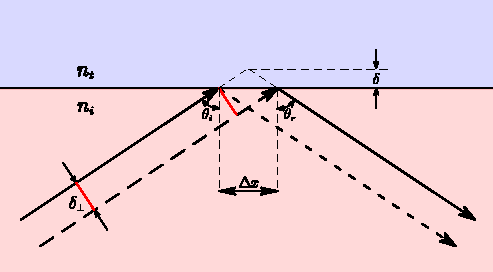
\includegraphics[width=0.8\columnwidth]{assets/1,2/GHShift.pdf}
\caption{ Goos-Hanchen Shift}\label{Goos-Hanchen Shift}
\end{figure}

\section{全反射时的相位变化}\label{全反射时的相位变化}


发生全内反射时\footnote{全内反射是指,由光疏介质射向光密介质且入射角大于临界角时发生的全反射现象},入射波 s 分量、p 分量的相位变化并非简单的 0 或 $\pi$,下面作推导。

对入射光的波函数 $\boldsymbol{E_i} = \boldsymbol{E_{i,0}} \cdot e^{i \theta} =\boldsymbol{E_{i,0}} \cdot e^{i(k x - \omega t)}$,若反射光满足 $\boldsymbol{E_{r}} = \boldsymbol{E_i}\cdot \lambda e^{i \delta}$,则表明相对于入射光,反射光的振幅变为了原来的 $\lambda$倍,且相位增加了 $\delta$。特别地,$\lambda < 0$ 时,可以等价于 $\lambda > 0$ 且相位增加 $\delta + \pi$ 或 $\delta - \pi$。

由菲涅尔定律,我们有 $\boldsymbol{E_{r,s}} = r_s \boldsymbol{E_{i,s}},\quad \boldsymbol{E_{r,p}} = r_p \boldsymbol{E_{i,p}}$。可以发现,在全反射时,$r_s, r_p \in \C \setminus \R$,并且 $| r_s | = | r_p | = 1$,振幅不变,于是可以令 $r = e^{i \delta }$。为了反解相位增量 $\delta $,一种自然的想法是考虑 
\begin{equation}
    e^{i \delta} = \cos \delta + i \lambda \sin \delta = a + ib \Longrightarrow  \delta =  \arctan \left( \frac{b}{a} \right)
\end{equation}

这样做虽然可行,但由于 $\arctan $ 函数的局限性,其值域范围在 $[-\frac{\pi}{2}, \frac{\pi}{2}]$,而 $\delta $ 的取值范围在 $[0, \pi]$ 或者 $[-\pi, 0]$。因此,最终得到的 $\delta$ 仅在部分区域上正确,对另一部分需做数学上的平移修正。因此,我们考虑另一种方法。在全反射时,注意到 $r_s$ 和 $r_p$ 的形式为 $r = \frac{a - bi}{a +bi}$,其中 $a, b \in \R$,有如下过程:
\begin{equation}
\frac{a - bi}{a + bi} = e^{i \theta} \Longrightarrow e^{i \frac{\theta}{2}} = \pm \frac{a - bi}{\sqrt{a^2 + b^2} },\ \tan \frac{\delta}{2} = - \frac{b}{a},\ \frac{\delta}{2} = \arctan \left( - \frac{b}{a} \right)
\end{equation}
这样得到的 $\frac{\delta}{2}$ 便是全范围正确的,无需修正。分别令 $r = r_s, r_p$,代入即得:
\begin{gather}
\delta_{r,s} = - 2 \arctan \left( \frac{\sqrt{\sin^2 \theta_i - n_{ti}^2} }{\cos \theta_i} \right) 
,\quad 
\delta_{r,p} = - 2 \arctan \left( \frac{\sqrt{\sin^2 \theta_i - n_{ti}^2} }{n_{21}^2 \cos \theta_i} \right)
\end{gather}

\section{折射时的相位变化}

入射光不发生全反射时,由菲涅尔定律,$t_s, t_p \in (0, \frac{2n_i}{n_i + n_t}) \subset \R$,恒为正实数,因此相位不发生任何变化。当入射光发生全反射时,折射光(透射光)以隐失波的形式存在,我们前面已经提过,隐失波同时含有横波纵波成分,它与入射光不再是同一种波,此时谈论相位变化自然没有意义。

\section{倒逆关系}

如图 \ref{光路可逆性下的振幅与能量系数},考虑光路可逆性,假设反射光、折射光振幅不变而方向置反,则合成出的光也应是原来的入射光(左下角合成后为 0),得到斯托克斯倒逆关系: 
\begin{equation}\label{斯托克斯倒逆关系}
r' + r = 1,\quad tt' + rr' = 1
\end{equation}
由于没有涉及电场的方向,上式对 $s$ 波、$p$ 波均成立,可以角标同时为 $s$,也可以角标同时为 $p$。

\begin{figure}[H]\centering
    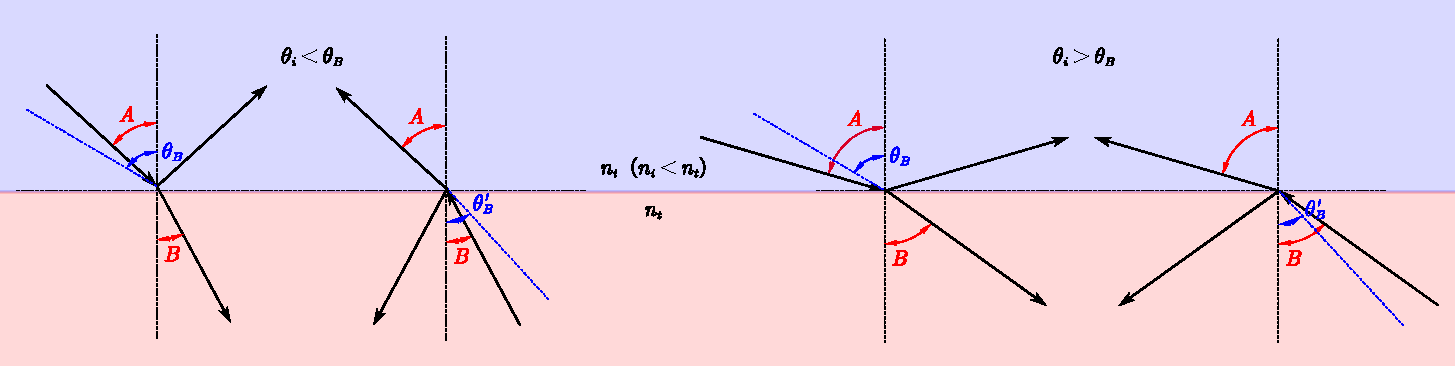
\includegraphics[width=\columnwidth]{assets/3/光路可逆性下的振幅与能量系数.pdf}
    \caption{ 光路可逆性下的振幅与能量系数}\label{光路可逆性下的振幅与能量系数}
\end{figure}

保持各角度不变,结合菲涅尔公式,可得对称前后(到逆前后)的各物理量变化:
\begin{gather}
r_s' = -r_s,\quad r_p' = -r_p \\ 
t_s' = \frac{n_t \cos \theta_t}{n_i \cos \theta_i} \cdot t_s,\quad t_p' = \frac{n_t \cos \theta_t}{n_i \cos \theta_i} \cdot t_p \\
R_s,\ R_p,\ R,\ T_s,\ T_p,\ T \ \text{均不变}
\end{gather}
式中的 $n_i$、$n_t$、$\theta_i$ 和 $\theta_t$ 都是倒逆之前的原始值。


\section{章末总结}

本章的所有结论基于电磁场的边界条件和麦克斯韦方程组,由菲涅尔定律推导而来,从波的角度揭示了光在反射折射时发生的变化,包括振幅、相位、能量、位移等关系。
\begin{align}
&\text{反射波:} \quad \boldsymbol{E_r} = \boldsymbol{E_{r,s}} + \boldsymbol{E_{r,p}} = r_s \boldsymbol{E_{i,s}} + r_p \boldsymbol{E_{i,p}},\quad  r \in \C 
\\ 
&\text{透射波:}\quad \boldsymbol{E_t} = \boldsymbol{E_{t,s}} + \boldsymbol{E_{t,p}} = t_s \boldsymbol{E_{i,s}} + t_p \boldsymbol{E_{i,p}},\quad  t \in \R,\ \theta_i < \theta_C
\\ 
& \text{反射系数:}
\begin{cases}\displaystyle
    r_s 
    = \frac{n_{{\color{red} i}} \cos \theta_{{\color{red} i}} - n_t \cos \theta_t}{n_{{\color{red} i}} \cos \theta_{{\color{red} i}} + n_t\cos \theta_t} 
    = \frac{\cos \theta_i - \sqrt{n_{ti}^2 - \sin^2 \theta_i} }{\cos \theta_i + \sqrt{n_{ti}^2 - \sin^2 \theta_i}}
    \\\displaystyle
    r_p 
    = \frac{n_t \cos \theta_{{\color{red} i}} - n_{{\color{red} i}} \cos \theta_t}{n_t \cos \theta_{{\color{red} i}} + n_{{\color{red} i}} \cos \theta_t} 
    =\frac{n_{ti}^2\cos \theta_i - \sqrt{n_{ti}^2 - \sin^2 \theta_i} }{n_{ti}^2\cos \theta_i + \sqrt{n_{ti}^2 - \sin^2 \theta_i}}
\end{cases}
\\ 
& \text{透射系数:} \quad  (-r_s) + t_s  = 1,\quad r_p + {\color{red} \frac{\cos \theta_t}{\cos \theta_i}}\cdot t_p = 1 
\\
& \text{能量关系:}
\begin{cases}
    R = \frac{1}{2}(R_s + R_p)\quad R_s = | r_s |^2,\ R_p = | r_p |^2 \\ 
    T = \frac{1}{2}(T_s + T_p),\quad 
    T_s = {\color{red} \frac{n_t \cos \theta_t}{n_i \cos \theta_i}} \cdot t_s^2, T_p = \frac{n_t \cos \theta_t}{n_i \cos \theta_i} \cdot t_p^2 \\
    R + T = 1 ,\ R_s + T_s = 1,\ R_p + T_p = 1 \\ 
    \Phi_{e,r} = R\Phi_{e,i},\ \Phi_{e,t} = T\Phi_{e,i}
\end{cases}
\\
& \text{$s$ 波反射相位增量:} 
\delta_{r,s} = 
\left\{\begin{matrix}
    -\pi, & n_i < n_t \\ 
    \begin{Bmatrix}
        0, & \theta_i \in (0, \theta_C)\\
        - 2 \arctan \left( \frac{\sqrt{\sin^2 \theta_i - n_{ti}^2} }{\cos \theta_i} \right), & \theta_i > \theta_C
    \end{Bmatrix}, & n_i > n_t
\end{matrix}\right.
\\
& \text{$p$ 波反射相位增量:} 
\delta_{r,p} = 
\left\{\begin{matrix}
    \begin{Bmatrix}
        0, & \theta_i \in (0, \theta_B) \\
        - \pi & \theta_i \in (\theta_B, \frac{\pi}{2})
    \end{Bmatrix}, & n_i < n_t 
    \\ 
    \begin{Bmatrix}
        -\pi, & \theta_i \in (0, \theta_B) \\
        0, & \theta_i \in (\theta_B, \theta_C) \\
        - 2 \arctan \left( \frac{\sqrt{\sin^2 \theta_i - n_{ti}^2} }{n_{ti}^2 \cos \theta_i} \right), & \theta_i \in (\theta_C, \frac{\pi}{2})
    \end{Bmatrix}, & n_i > n_t
\end{matrix}\right.
\\
&\text{隐失波:} \boldsymbol{E_{t}} = \left( e^{-\beta y} \boldsymbol{E_{t,0}}\right)\cdot e^{i\left( \frac{\sin \theta_i}{n_{ti}}  k_t x - \omega t \right)},\quad \beta  = k_i\sqrt{\sin^2 \theta_i - n_{ti}^2} = \frac{2 \pi}{\lambda_i} \sqrt{\sin^2 \theta_i - n_{ti}^2},\quad \delta = \frac{1}{\beta}
\\ 
& \text{Goos-Hanchen Shift: \ } \quad \Delta x = 2 \delta \tan \theta_i = \frac{2 \tan \theta_i}{k_i\sqrt{\sin^2 \theta_i - n_{ti}^2}}
= \frac{\lambda_i \tan \theta_i }{\pi \sqrt{\sin^2 \theta_i - n_{ti}^2} }
\\ 
& \ \text{倒逆关系:} 
\begin{cases}
    r_s' = -r_s,\quad r_p' = -r_p \\ 
    t_s' = \frac{n_t \cos \theta_t}{n_i \cos \theta_i} \cdot t_s,\quad t_p' = \frac{n_t \cos \theta_t}{n_i \cos \theta_i} \cdot t_p \\
    R_s,\ R_p,\ R,\ T_s,\ T_p,\ T \ \text{均不变}
\end{cases}
\end{align}



在下一页中给出了上面结论的相关图像。图 \ref{反射折射光的振幅与能量变化}\footnote{源码见附录 \ref{反射折射光的振幅与能量变化 源码}} 展示了反射折射光的振幅 $r_s, r_p, t_s, t_p$、能量 $R_s, R_p, R$ 随入射角 $\theta_i$ 的变化。
图 \ref{反射光 s 分量与 p 分量的相位增量}\footnote{源码见附录 \ref{反射光 s 分量与 p 分量的相位增量 源码}} 展示了反射光的 s 分量与 p 分量的相位增量 $\delta_{r,s}, \delta_{r,p}$ 随入射角 $\theta_i$ 的变化。特别地,当 图 \ref{反射光 s 分量与 p 分量的相位增量} (b) 中 $\theta_i > \theta_C$ 时,发生全(内)反射,此时 $r_s, r_p, t_s, t_p \in \C \setminus \R$ ,图中展示的是它们的模长,即 $|r_s|, |r_p|, |t_s|, |t_p|$。
图 \ref{隐失波穿透深度与 GH Shift 玻璃入射空气}\footnote{源码见附录 \ref{隐失波穿透深度与 GH Shift 玻璃入射空气 源码}} 展示了隐失波穿透深度 $\delta$ 和 GH Shift $\Delta x$ 随入射角 $\theta_i$ 的变化。


\newpage
\begin{figure}[H]\centering
\begin{subfigure}[t]{0.44\columnwidth}\centering
    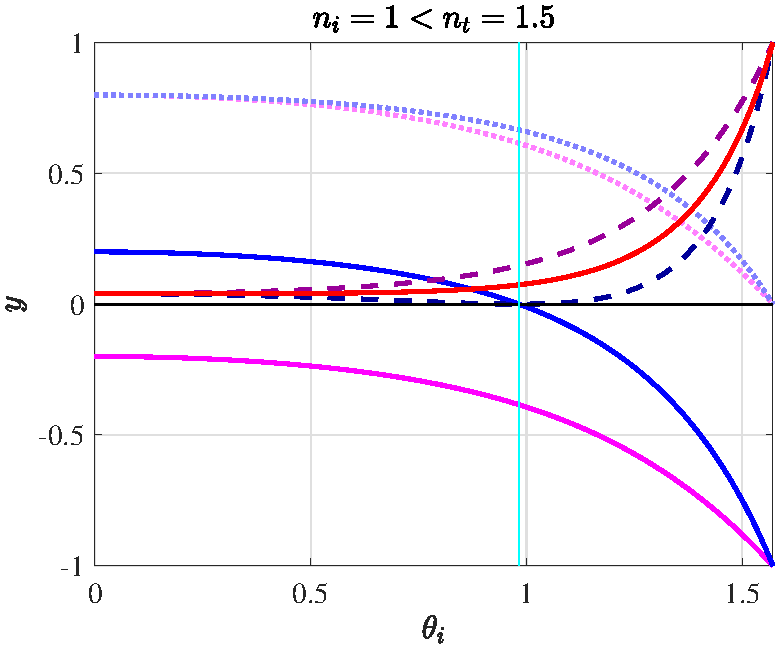
\includegraphics[height=170pt]{assets/1,2/2024-09-21_12-26-37.pdf}
    \caption{ 由空气入射玻璃 }
\end{subfigure}
\subcaptionsetup{
    margin={2cm,0cm}, % 右边距不变,左边距为 2cm
    %labelsep=period % 标签与标题内容之间的分隔符为点号
    }
\begin{subfigure}[t]{0.54\columnwidth}\centering
    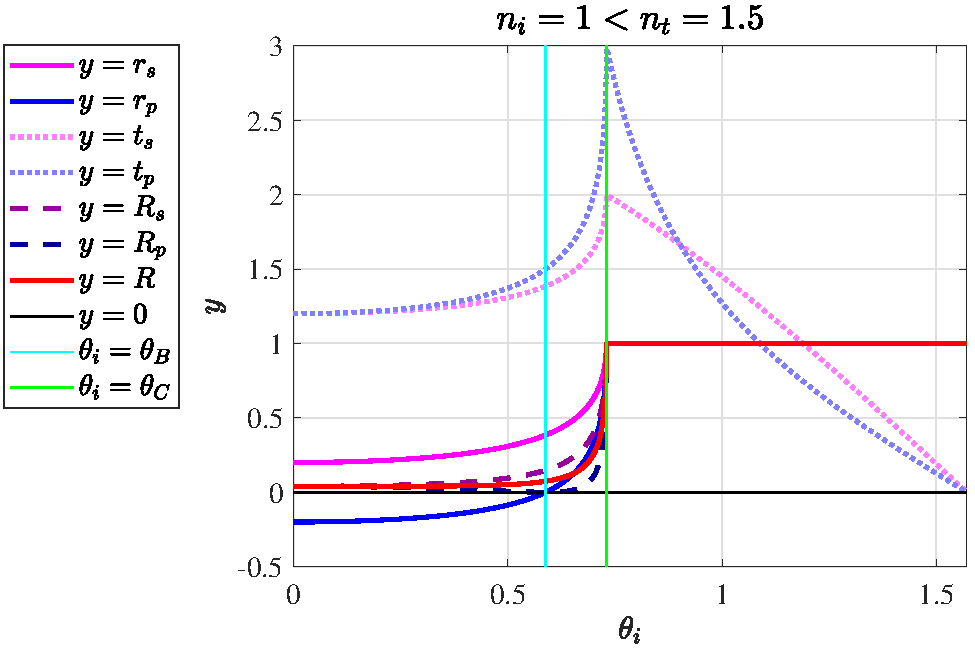
\includegraphics[height=170pt]{assets/1,2/2024-09-21_12-31-00.pdf}
    \caption{ 由玻璃入射空气 }
\end{subfigure}
\caption{ 反射折射光的振幅与能量变化 }
\label{反射折射光的振幅与能量变化}
\end{figure}

\begin{figure}[H]\centering
\begin{subfigure}[t]{0.5\columnwidth}\centering
    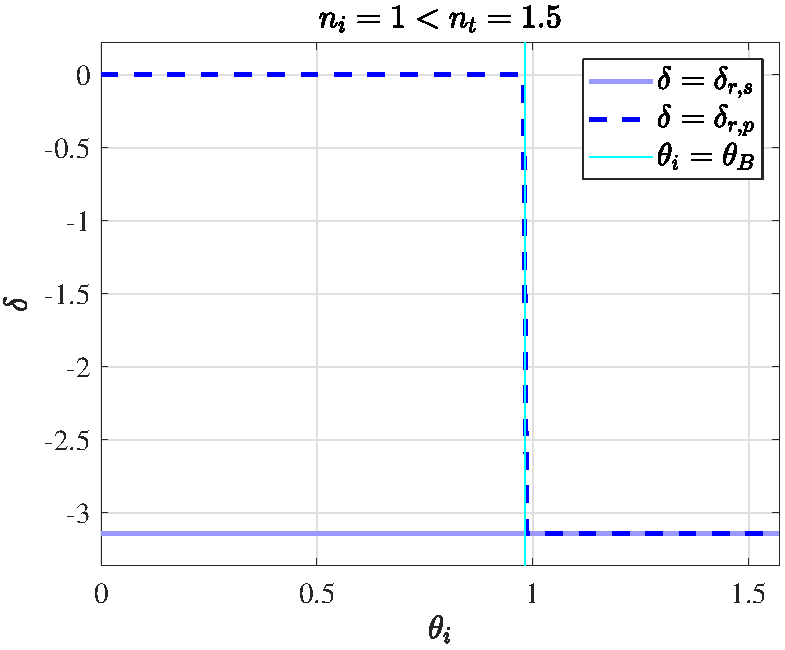
\includegraphics[height=175pt]{assets/1,2/光疏到光密.pdf}
    \caption{ 由空气入射玻璃 }
\end{subfigure}\begin{subfigure}[t]{0.5\columnwidth}\centering
    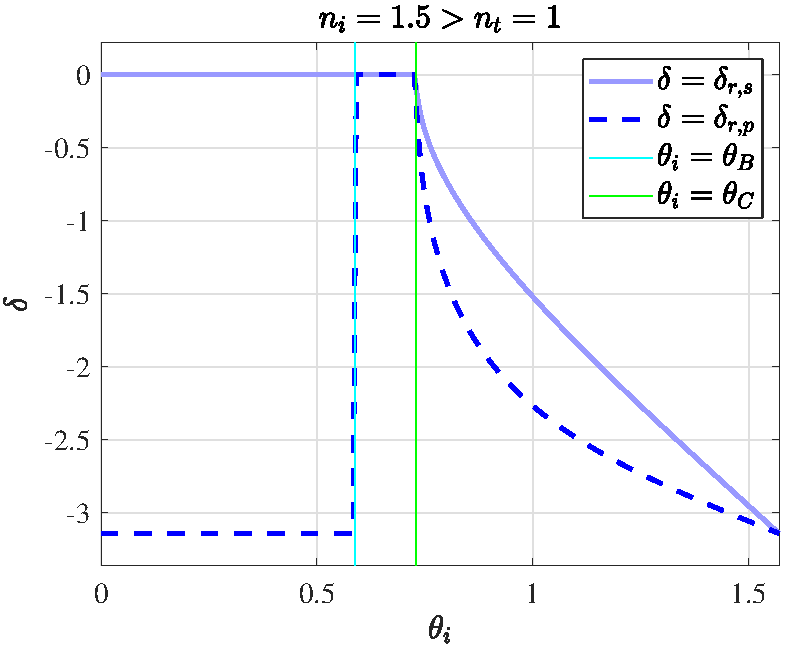
\includegraphics[height=175pt]{assets/1,2/光密到光疏.pdf}
    \caption{ 由玻璃入射空气 }
\end{subfigure}
\caption{ 反射光 s 分量与 p 分量的相位增量 }
\label{反射光 s 分量与 p 分量的相位增量}
\end{figure}

\begin{figure}[H]\centering
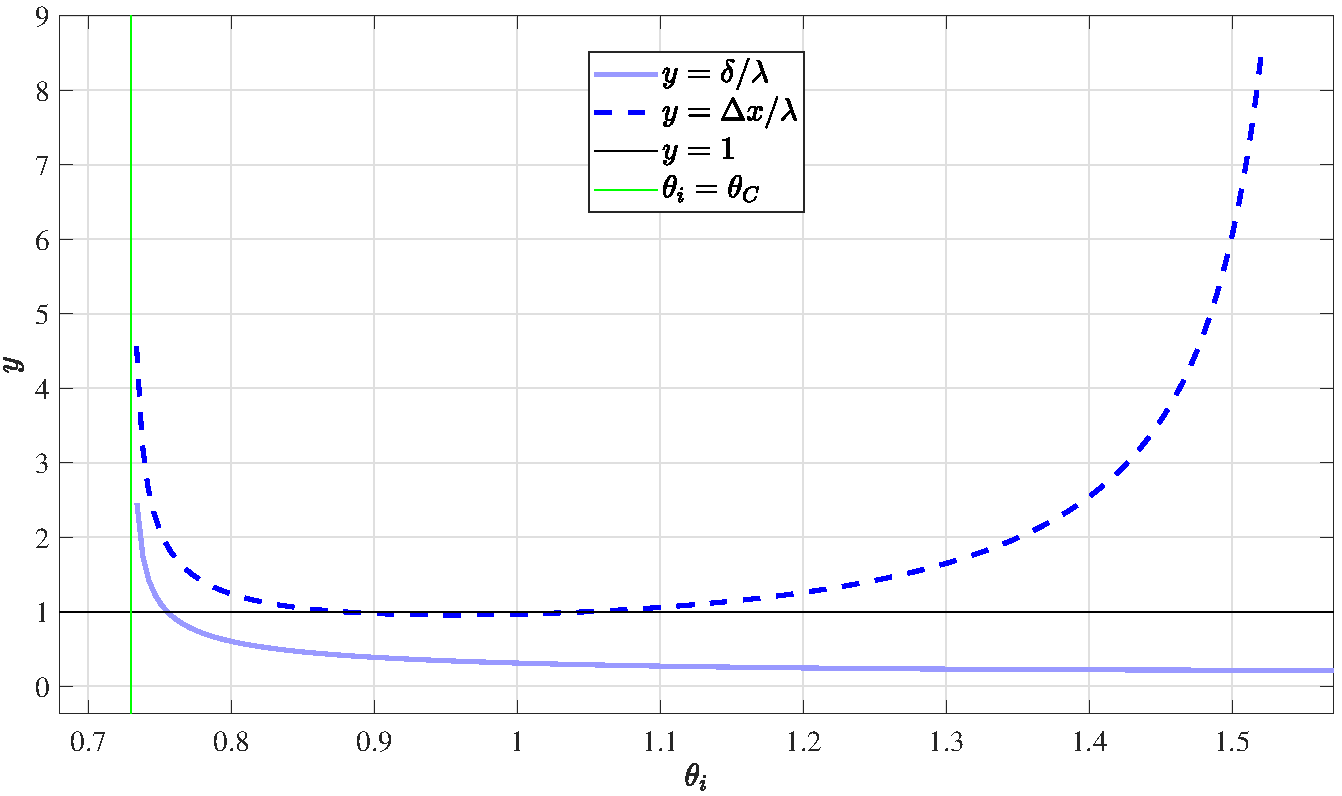
\includegraphics[width=0.70\columnwidth]{assets/1,2/2024-09-21_13-29-49.pdf}
\caption{ 隐失波穿透深度与 GH Shift(玻璃入射空气)}\label{隐失波穿透深度与 GH Shift 玻璃入射空气}
\end{figure}


\chapter{光的干涉}\thispagestyle{fancy}


通常将平面波与球面波\footnote{即平面电磁波与球面电磁波,详见附录 \ref{平面波、柱面波与球面波},也可参考 \href{https://www.zhihu.com/question/267133640/answer/319531458}{知乎:球面光波与平面光波} 和 \href{https://www.zhihu.com/question/534511391/answer/2501271591}{知乎:高斯光束,平面波,球面波三者间有什么关系}}是光波的的基元,当两个光源(或两束光波)间存在某种关联,波的叠加会引起强度的重新分布,若相互叠加的波满足某些特定条件,使得叠加后产生了稳定的强度分布,则称发生了光的干涉。

换句话说,研究干涉现象,就是讨论当两个或多个(光)波在空间中的某区域相遇时,它们如何相互叠加,会产生怎样的新波动现象,了解各个波的特性(振幅、频率、相位、波的类型等)如何影响叠加后的波的性质。



\section{叠加原理}
只要波在空间中某点相遇,就会发生叠加,但不一定会产生干涉。也就是说,叠加是无条件的,干涉则要求形成稳定的、新的强度分布。

回想波动方程\footnote{详见附录 \ref{波动方程}},它的一个重要特性是:方程是线性的。因此,如果 $\boldsymbol{\psi_1},\ \boldsymbol{\psi_2},\ ...,\ \boldsymbol{\psi_n}$ 各自是波动方程的解,那么它们的任意线性组合也是方程的解,即:
\begin{equation}
\boldsymbol{\psi} = \sum a_i \boldsymbol{\psi_i}
\end{equation}

这个性质称为叠加原理,它表面:介质中任何一点的合扰动是各个单独波组分的代数和。另外,需要注意,叠加原理仅在均匀、线性、各向同性的介质中成立,有极大振幅的波(能量极大),无论是纵波(声波)或横波(电磁波),都可以产生非线性的效应,此时叠加原理不再适用。

在许多情况下,无需考虑光波的矢量性,例如多个光波的电场方向都始终在一条直线上时,可以将电场 $\boldsymbol{E}$ 处理为具有正负的标量 $E$。本章我们研究的都是基于上述处理的光波,这表明它们的传播方向都在同一平面内,这样即降低了讨论的难度,又具有相当高的普适性和推广性(利用旋转对称性或平移对称性)。

\section{同频率光波的干涉}

\subsection{两个同频波源的干涉}

\subsubsection{两源干涉原理:}

现在,我们讨论均匀介质的两个波源(频率相同)的干涉情况,为了提高普适性,我们并不事先假设波源的类似,它可以是平面波、球面波或柱面波。设两波源分别为 $S_A, S_B$,波函数分别为 $\psi_A, \psi_B$,不妨假设它们都沿各自的正向传播,借助相矢量的思想\footnote{详见附录 \ref{相矢量}},将位矢 $\boldsymbol{x}$ (和初相位 $\varepsilon$)分离后,它们的波函数可写为:
\begin{equation}
    E_A = E_{A,0}\cdot e^{i(-\omega t + \alpha_A)},\quad E_B = E_{B,0}\cdot e^{i(-\omega t + \alpha_B)}
\end{equation}
其中 $\alpha_A = \alpha_A(\boldsymbol{x})$,$\alpha_B = \alpha_B(\boldsymbol{x})$ 是位矢的函数,$E_{A,0}, E_{B,0}$ 可能是位矢的函数。对于平面中任意一点 $P$,合扰动为:
\begin{equation}
E = E_A + E_B = E_{A,0}\cdot e^{i(-\omega t + \alpha_A)} + E_{B,0}\cdot e^{i(-\omega t + \alpha_B)}
\end{equation}
作数学上的处理,得到合扰动:
\begin{gather}
    E = E_0 \cos \left(-\omega t + \alpha \right) = E_0 \cdot e^{i(-\omega t + \alpha)}\\ 
    E_0 = \sqrt{E_{A,0}^2 + E_{B,0}^2 + 2E_{A,0}E_{B,0}\cos(\alpha_A - \alpha_B)},\quad 
    \begin{cases}
        \sin \alpha = \frac{1}{E_0}\left( E_{A,0}\sin \alpha_A + E_{B,0}\sin \alpha_B \right) \\
        \cos \alpha = \frac{1}{E_0}\left( E_{A,0}\cos \alpha_A + E_{B,0}\cos \alpha_B \right) 
    \end{cases} \\ 
    \alpha = 
    \begin{cases}
        \arcsin \left[ \frac{1}{E_0}\left( E_{A,0}\sin \alpha_A + E_{B,0}\sin \alpha_B \right)  \right] &, \cos \alpha \geqslant 0 \\
        \pi - \arcsin \left[ \frac{1}{E_0}\left( E_{A,0}\sin \alpha_A + E_{B,0}\sin \alpha_B \right)  \right] &,  \cos \alpha < 0
    \end{cases}
\end{gather}
$E_0$ 与 $\alpha$ 的取值可以由相矢量相加来理解。在给定的位置 $P$,$A$ 波的相矢量为 $E_{A,0}\measuredangle \alpha_A$,$B$ 波的相矢量为 $E_{B,0}\measuredangle \alpha_B$,在复平面中将它们相加(平行四边形法则),即得到合扰动的相矢量  $E_0\measuredangle \alpha$,这样,$E_0$ 的大小就是合相矢量的模长,$\alpha$ 是合相矢量与 $x$ 轴的夹角。

在光学中,常用干涉条纹对比度 $\gamma$ 来描述干涉情况是否明显,它定义为:
\begin{equation}
    \gamma = \frac{I_{\text{max}} - I_{\min}}{I_{\text{max}} + I_{\min}} = \frac{ E_{0,\text{max}}^2 -  E_{0,\min}^2 }{E_{0,\text{max}}^2 +  E_{0,\min}^2}
\end{equation}
其中 $I$ 表示光强,也即光通量密度。在两波源产生的干涉中,有:
\begin{gather}
I = I_1 + I_2 + 2 \sqrt{I_1I_2}\cos (\alpha_A - \alpha_B) \\ 
I_{\text{max}} = I_1 + I_2 + 2\sqrt{I_1I_2},\quad I_{\min} =  I_1 + I_2 - 2\sqrt{I_1I_2}
\end{gather}
则对比度为:
\begin{equation}
\gamma = \frac{2  }{ \sqrt{\frac{I_1}{I_2}}  + \sqrt{\frac{I_2}{I_1}}} = \frac{ 2  }{  \sqrt{\frac{E_{A,0,\text{max}}^2}{E_{B,0,\text{max}}^2}} + \sqrt{\frac{E_{B,0,\text{max}}^2}{E_{A,0,\text{max}}^2}}}
\end{equation}
因此,两波源电场的振幅越接近,干涉对比度越高,也就越明显。

\subsubsection{示例一:两球面波}

如图 \ref{两个同频波源的干涉} (a),考虑两个相同的球面波源在 $x$-$y$ 平面上的干涉情况,相同的波源(理想单频波源)保证了两束波的物理参数相同,如波长、频率和振幅等。设两波源位置分别为 $\boldsymbol{x_{OA}}$,$\boldsymbol{x_{OB}}$,简记 $ r_1 = | \boldsymbol{x}_{AP} |$ 和 $ r_2 = | \boldsymbol{x}_{BP} |$,则波函数可写为:
\begin{gather}
E_A = \frac{A}{r_1 } \cdot e^{i(-\omega t + k r_1 + \varepsilon_A)},\quad E_{A,0} = \frac{A}{r_1 },\ \alpha_A = k r_1 + \varepsilon_A
\\
E_B = \frac{B}{ r_2 } \cdot e^{i(-\omega t + k r_2  + \varepsilon_B)}\quad E_{B,0} = \frac{B}{ r_2 },\ \alpha_B = k r_2  + \varepsilon_B
\end{gather}

\begin{figure}[H]\centering
    \begin{subfigure}[t]{0.49\columnwidth}\centering
        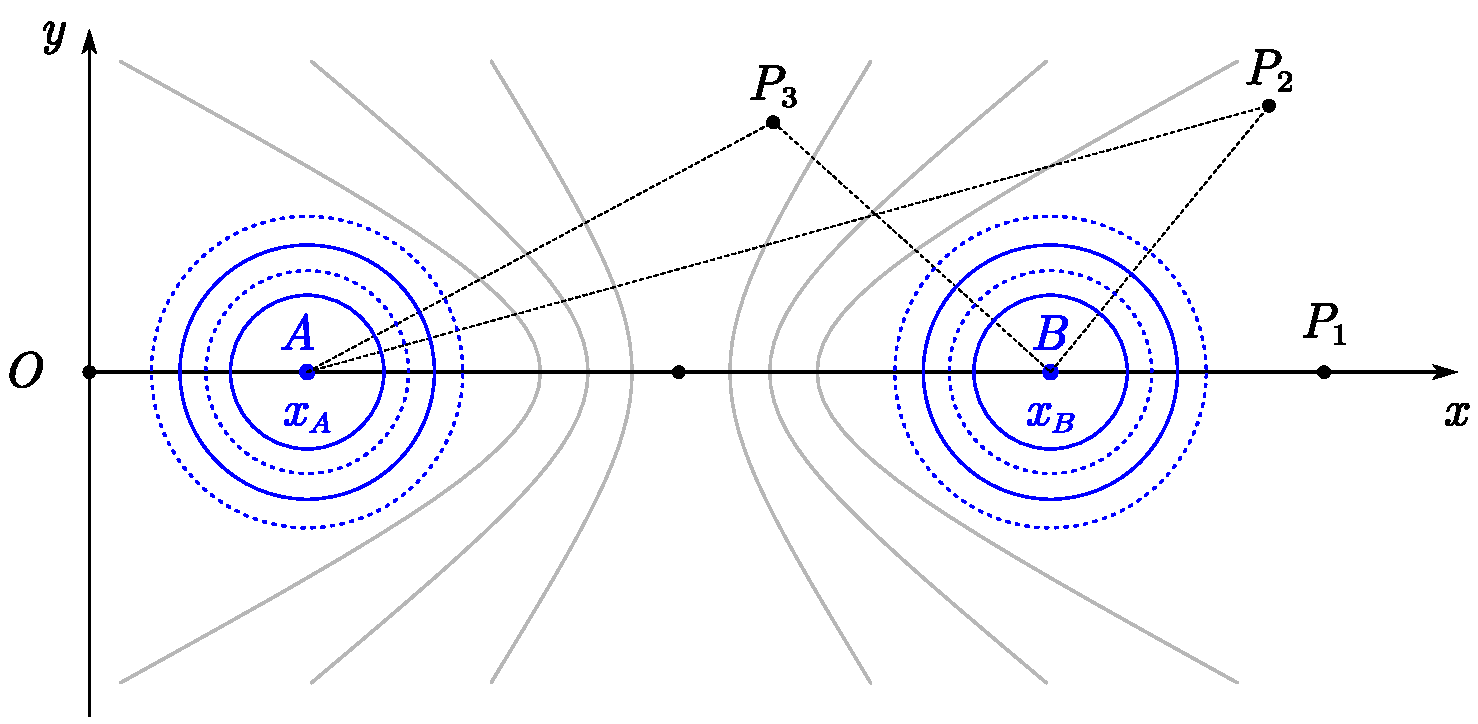
\includegraphics[height=120pt]{assets/3/两球面波源或两柱面波源.pdf}
        \caption{ 两球面波源或两柱面波源 }
    \end{subfigure}\hfill
    \begin{subfigure}[t]{0.49\columnwidth}\centering
        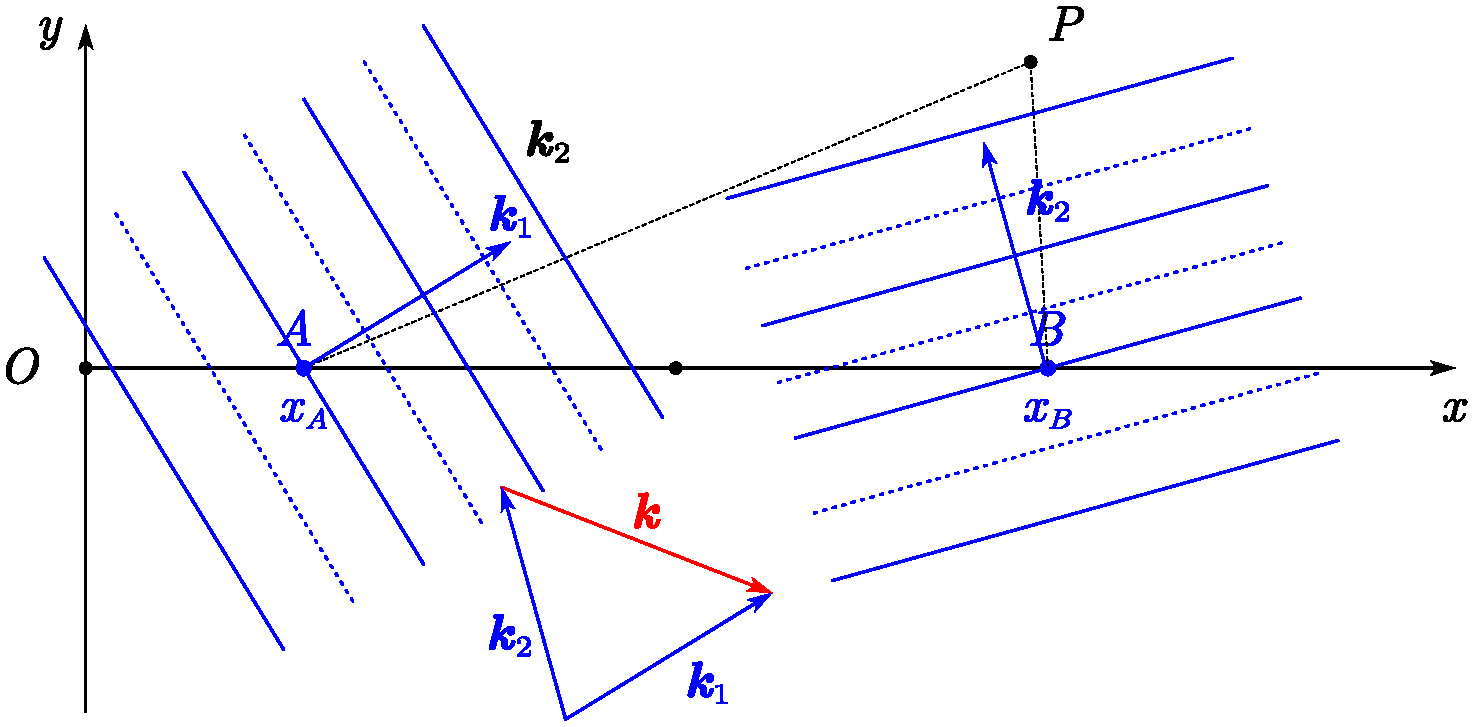
\includegraphics[height=120pt]{assets/3/双平面波源.pdf}
        \caption{ 两平面波源 }
    \end{subfigure}
    \caption{ 两个同频波源的干涉 }\label{两个同频波源的干涉}
\end{figure}


方便起见,不妨令 $\varepsilon_A = \varepsilon_B$,则合扰动为:
\begin{gather}
E = E_0 \cos \left(-\omega t + \alpha \right) = E_0 \cdot e^{i(-\omega t + \alpha)},\quad E_0 = \sqrt{\frac{A^2}{r_1^2} + \frac{B^2}{r_2^2} + \frac{2AB}{r_1r_2}\cos\left( k \left( r_1  - r_2 \right)\right)} \\ 
\sin \alpha = \frac{1}{E_0} \left( \frac{A}{ r_1 }\sin \alpha_A + \frac{B}{ r_2 } \sin \alpha_B\right),\quad \cos \alpha = \frac{1}{E_0} \left( \frac{A}{ r_1 }\cos \alpha_A + \frac{B}{ r_2 } \cos \alpha_B\right)\\ 
\alpha = 
\begin{cases}
    \arcsin \left[ \frac{1}{E_0} \left( \frac{A}{ r_1 }\sin \alpha_A + \frac{B}{ r_2 } \sin \alpha_B\right) \right] &, \cos \alpha \geqslant 0 \\
    \pi - \arcsin \left[ \frac{1}{E_0} \left( \frac{A}{ r_1 }\sin \alpha_A + \frac{B}{ r_2 } \sin \alpha_B\right) \right] &,  \cos \alpha < 0
\end{cases}
\end{gather}


对于可见光,其波长在 nm 级别,空间频率 $k = \frac{2\pi}{\lambda}$ 极高。为方便可视化,我们取波长 $\lambda = 0.4 \pi \ \mathrm{m}$,即 $k = 5$ 的微波,并令振幅系数 $A = 50$,$B = 50$,作出图像。图 \ref{单个球面波源在平面上的振荡情况}\footnote{源码见附录 \ref{单个球面波源在平面上的振荡情况 源码}} 展示了单个波源在平面上的振荡情况($t = 0$)。对两波源的干涉,我们令两波源位置分别为 $(-2, 0)$,$(2, 0)$,作出图像,图 \ref{两个球面波源在平面上的干涉情况}\footnote{源码见附录 \ref{两个球面波源在平面上的干涉情况 源码}} 展示了它们的干涉情况($t = 0$)。单波源和双波源随时间的振动详见 GIF 动图链接 \href{https://www.123pan.com/s/0y0pTd-QwKj3}{https://www.123pan.com/s/0y0pTd-QwKj3}。

\begin{figure}[H]\centering
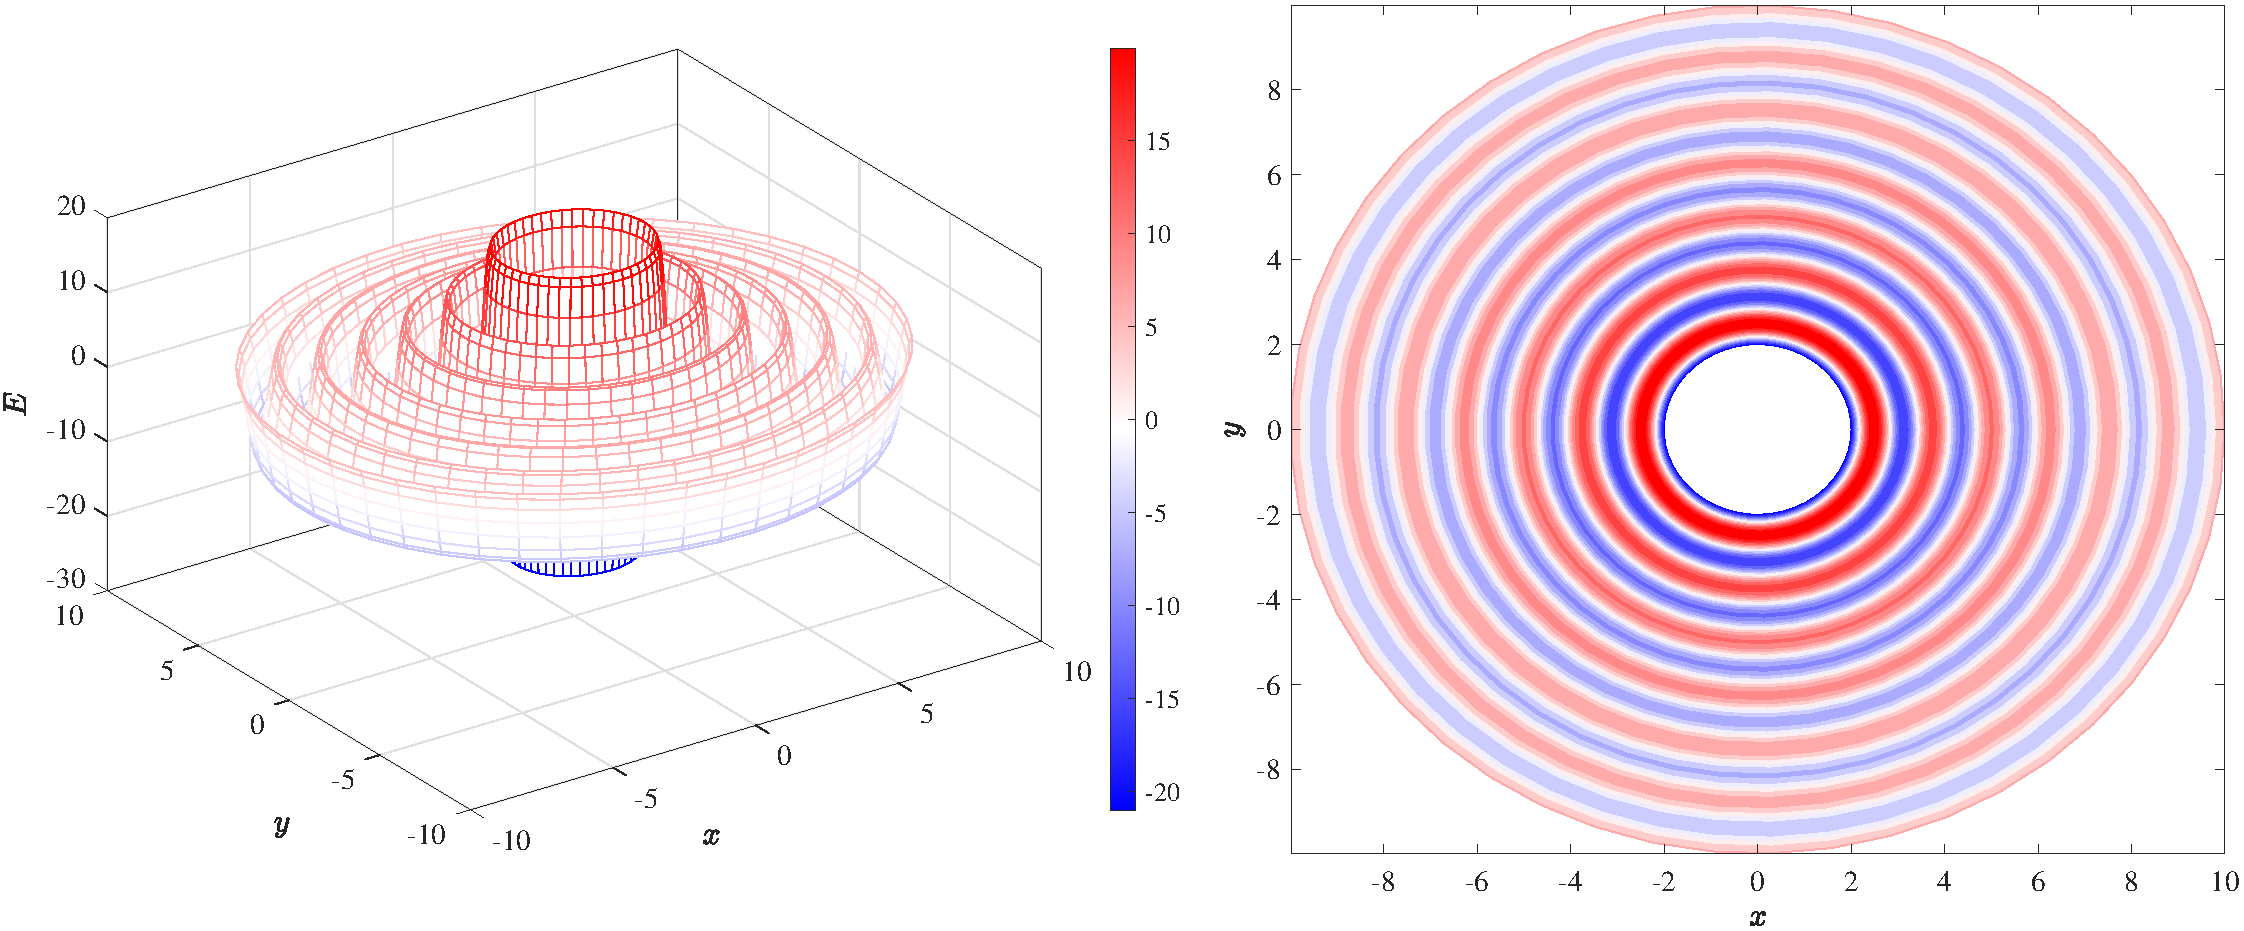
\includegraphics[width=0.95\columnwidth]{assets/3/单个球面波源.pdf}
\caption{ 单个球面波源在平面上的振荡情况}\label{单个球面波源在平面上的振荡情况}
\end{figure}

\begin{figure}[H]\centering
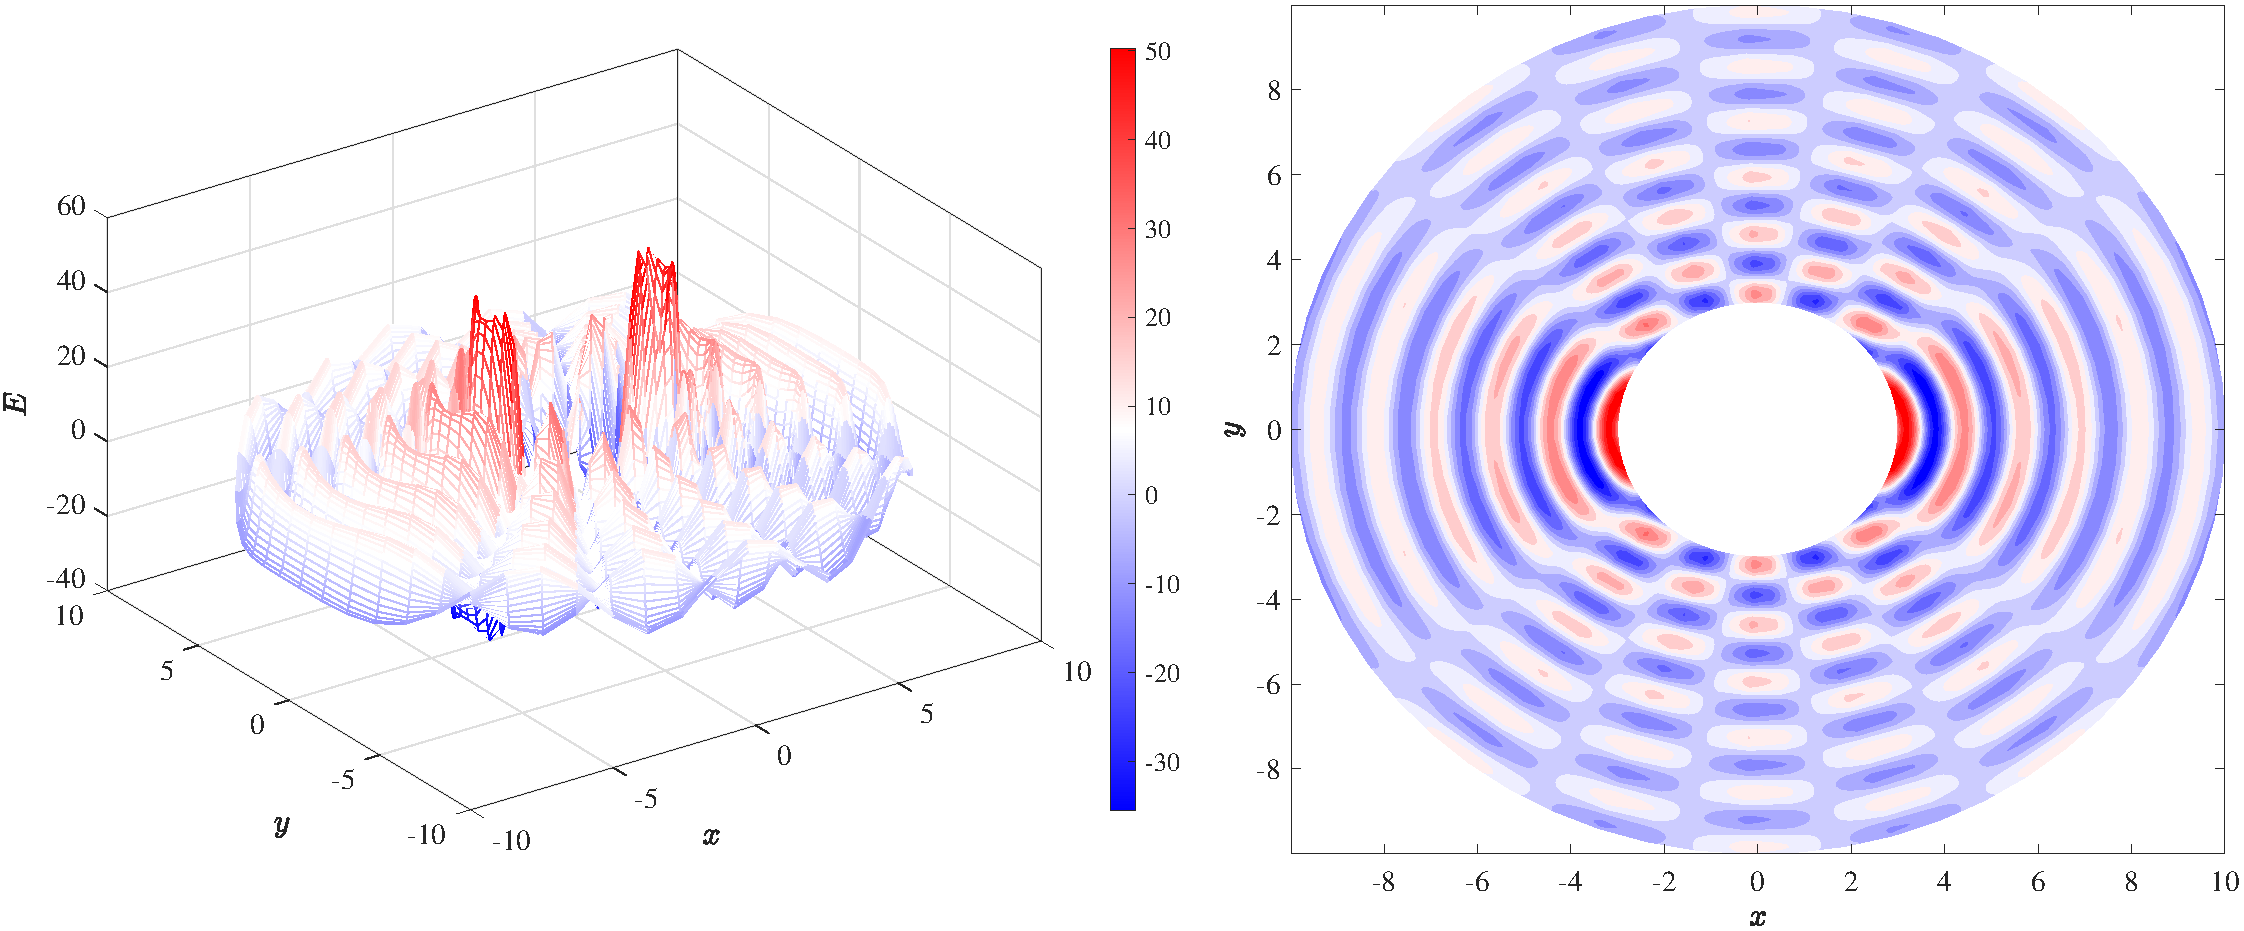
\includegraphics[width=0.95\columnwidth]{assets/3/两个球面波源.pdf}
\caption{ 两个球面波源在平面上的干涉情况}\label{两个球面波源在平面上的干涉情况}
\end{figure}

当点 $P$ 离波源极远时,近似有 $\frac{r_1}{r_2} = 1$(这与近似有 $r_1 - r_2 = 0$ 不同),将距离记为 $r$,则振幅的位置分布为 $E_0 = \frac{1}{r} \sqrt{ A^2 + B^2 + 2AB \cos (k(r_1 - r_2))} $。若可以认为 $\frac{1}{r}$ 近似不变,则此时,具有相同振幅大小的点,等价于 $\cos (k(r_1 - r_2))$ 具有相同的值,也即:
\begin{equation}
    | r_1 -  r_2| =  \frac{1}{k} (\theta + 2\pi n),\quad \theta \in [0, 2\pi),\  n = 0,1,2,\cdots
\end{equation}

对每个给定的 $n$,上述方程表示一条双曲线(焦点为两波源),因此上述方程构成一个双曲线族(空间中构成旋转双曲面族),如图 \ref{两个同频波源的干涉} (a) 中的灰色曲线所示。特别地,令 $\theta = 0$ 可以得到最大振幅对应的双曲线族,令 $\theta = \pi$,得到最小振幅对应的双曲线族。

由于球面波的旋转对称性,只需绕 $x$ 轴旋转一圈,即可得到整个空间上的振幅分布情况,也即两波源干涉情况。振幅的位置分布是较为重要的内容,在后文的干涉实验部分,我们将再次讨论这个问题。


\subsubsection{示例二:两柱面波}

考虑两柱面波的干涉情况,其中柱体的高与 $x$-$y$ 平面垂直。容易发现,这与球面波在 $x$-$y$ 平面的行为是相同的,仅需修改波源的振幅衰减系数。同样地,不妨令初相位 $\varepsilon_1 = \varepsilon_2$,得到合扰动:

\begin{gather}
    E = E_0 \cos \left(-\omega t + \alpha \right) = E_0 \cdot e^{i(-\omega t + \alpha)},\quad E_0 = \sqrt{\frac{A^2}{r_1} + \frac{B^2}{r_2} + \frac{2AB}{\sqrt{r_1r_2} }\cos\left( k \left( r_1  - r_2 \right)\right)} \\ 
    \sin \alpha = \frac{1}{E_0} \left( \frac{A}{ \sqrt{r_1} }\sin \alpha_A + \frac{B}{ \sqrt{r_2} } \sin \alpha_B\right),\quad \cos \alpha = \frac{1}{E_0} \left( \frac{A}{ \sqrt{r_1} }\cos \alpha_A + \frac{B}{ \sqrt{r_2} } \cos \alpha_B\right)\\ 
    \alpha = 
    \begin{cases}
        \arcsin \left[ \frac{1}{E_0} \left( \frac{A}{ \sqrt{r_1} }\sin \alpha_A + \frac{B}{ \sqrt{r_2} } \sin \alpha_B\right) \right] &, \cos \alpha \geqslant 0 \\
        \pi - \arcsin \left[ \frac{1}{E_0} \left( \frac{A}{ \sqrt{r_1} }\sin \alpha_A + \frac{B}{ \sqrt{r_2} } \sin \alpha_B\right) \right] &,  \cos \alpha < 0
    \end{cases}
\end{gather}
由于柱面波的平移对称性,只需沿 $z$ 轴进行平移,即可得到整个空间上的干涉情况。在平面内的其它性质与球面波类似。

\subsubsection{示例三:两平面波}

考虑两平面波的干涉情况,如图 \ref{两个同频波源的干涉} (b),平面波函数为:
\begin{gather}
    E_A = E_{A,0}\cdot e^{i(-\omega t + k r_1 + \varepsilon_A)},\quad \ \alpha_A = \boldsymbol{k_1}  \cdot  \boldsymbol{x}_{AP} + \varepsilon_A
    \\
    E_B = E_{B,0} \cdot e^{i(-\omega t + k r_2  + \varepsilon_B)}\quad  \alpha_B = \boldsymbol{k_2} \cdot \boldsymbol{x}_{BP}  + \varepsilon_B
\end{gather}
令 $\varepsilon_1 = \varepsilon_2$,得到合扰动:
\begin{gather}
    E = E_0 \cos \left(-\omega t + \alpha \right) = E_0 \cdot e^{i(-\omega t + \alpha)} \\ 
    E_0 = \sqrt{E_{A,0}^2 + E_{B,0}^2 + 2 \cos \left( \Delta \alpha \right)} ,\quad \Delta \alpha =  (\boldsymbol{k_1} -\boldsymbol{k_2})\cdot \boldsymbol{x} + (\boldsymbol{k_2}\cdot \boldsymbol{x}_B - \boldsymbol{k_1} \cdot \boldsymbol{x}_A)\\ 
        \sin \alpha = \frac{1}{E_0}\left[ E_{A,0}\sin ( \boldsymbol{k_1}  \cdot  \boldsymbol{x}_{AP}) + E_{B,0}\sin (\boldsymbol{k_2} \cdot \boldsymbol{x}_{BP}) \right] \\ 
        \cos \alpha = \frac{1}{E_0}\left[ E_{A,0}\cos ( \boldsymbol{k_1}  \cdot  \boldsymbol{x}_{AP}) + E_{B,0}\cos (\boldsymbol{k_2} \cdot \boldsymbol{x}_{BP}) \right] \\ 
    \alpha = 
    \begin{cases}
        \arcsin \left[ \frac{1}{E_0}\left( E_{A,0}\sin \alpha_A + E_{B,0}\sin \alpha_B \right)  \right] &, \cos \alpha \geqslant 0 \\
        \pi - \arcsin \left[ \frac{1}{E_0}\left( E_{A,0}\sin \alpha_A + E_{B,0}\sin \alpha_B \right)  \right] &,  \cos \alpha < 0
    \end{cases}
\end{gather}

由于 $\boldsymbol{k_1} \cdot \boldsymbol{x}_A$ 和 $\boldsymbol{k_2} \cdot \boldsymbol{x}_B$ 是定值,而 $\boldsymbol{k} = \boldsymbol{k_1} - \boldsymbol{k_2}$ 构成一个新的传播矢量,因此合成后的波仍是平面波(但不均匀,振幅是位置的函数),或者说每个等相面仍构成一个平面。

类似地,由平面波的平移对称性,沿 $z$ 轴平移即可得全空间的合成情况。

\subsection{多个同频波源的干涉}

上面的结论容易推广到任意 $n$ 个扰动叠加,即:
\begin{gather}
    E = E_0 \cos \left(-\omega t + \alpha \right) = E_0 \cdot e^{i(-\omega t + \alpha)}
    \\ 
    E_0 = \sqrt{\left( \sum_{i=1}^n E_{i,0}\sin \alpha_i \right)^2 + \left( \sum_{i=1}^n E_{i,0}\cos \alpha_i \right)^2 }   \\ 
    =  \sqrt{\sum_{i=1}^n E_{i,0}^2 + \sum_{1 <= i < j <= n} 2E_{i,0}E_{j,0}\cos(\alpha_i - \alpha_j)},\quad
    \\ 
    \sin \alpha = \frac{1}{E_0}\sum_{i=1}^n E_{i,0}\sin \alpha_i ,\quad 
    \cos \alpha = \frac{1}{E_0}\sum_{i=1}^n E_{i,0}\cos \alpha_i \\ 
    \alpha = 
    \begin{cases}
        \arcsin \left( \frac{1}{E_0}\sum_{i=1}^n E_{i,0}\sin \alpha_i  \right) &, \cos \alpha \geqslant 0 \\
        \pi - \arcsin \left( \frac{1}{E_0}\sum_{i=1}^n E_{i,0}\cos \alpha_i  \right) &,  \cos \alpha < 0
    \end{cases} \\ 
    I = \sum_{i=1}^n I_i + \sum_{1 <= i < j <= n} 2\sqrt{I_iI_j} \cos(\alpha_i - \alpha_j) 
\end{gather}

\section{不同频率光的干涉(略)}

\section{产生干涉的前提条件}\label{产生干涉的前提条件}

前面我们已经提到,在叠加(或干涉)问题中,电场的振幅通常只是位置的函数,而与时间无关,其实这也是观察到干涉图样的必要条件。观察干涉图样,无非是用照片(视频等同于照片)、人眼、辐射计以及类似的传感器,它们都有一定的“曝光时间”,我们只能观察到在曝光时间内,光强或辐射强度的平均值。
其中 $\tau$ 为仪器的曝光时间。可见光的简谐周期 $T = \frac{\lambda}{v}$ 在 $10^{-15}$ s 级别,因此曝光时间 $\tau$ 通常远大于 $T$,于是我们只能观察到平均光强,而无法观察到光强的瞬时变化,即:
\begin{equation}
I = I_1 + I_2 + 2 \sqrt{I_1 I_2} \cdot \frac{1}{\tau} \int_{0}^{\tau}  \cos(\Delta \alpha) \mathrm{d} t =  I_1 + I_2 + 2 \sqrt{I_1 I_2} \cdot \langle \cos \Delta \alpha \rangle_\tau
\end{equation}
如果 $\Delta \alpha$ 与时间无关(这对波列长度有要求),或者在曝光时间内几乎保持不变,那么就能得到(观察到)稳定的干涉图样。否则恒有 $I = I_1 + I_2$,是平凡的叠加,称为非相干叠加。另外,若两波源的振动方向垂直,电场也仅是平凡的叠加,而不会产生干涉。因此,干涉现象要求两波源振动方向不能垂直。

以能发射单频波的普通光源为例,光是由光源中的原子发生能级跃迁时发出的,原子跃迁时发出的波列长都有限,且初相位随机,持续时间 $\tau_0$ 通常短于 10 ns,在此时段内,光场振荡约百万次。对于探测设备来讲,10 ns 通常极短,远远小于曝光时间,也即 $\tau \ll \tau_0 \ll T$。

%\footnote{即光谱宽度极短,光谱宽度对对比度的影响详见 \ref{多色光源迈克尔逊干涉} 节“多色光源迈克尔逊干涉”的公式 \ref{光谱宽度对对比度的影响}}

现在假设光源的单色性极好,考虑被分波前或分振幅而导致具有光程差的两束相干光的叠加,此时,相位差 $\Delta \alpha$ 随时间 $t$ 的变化仅取决于波列长度 $L_0 = c \tau_0$。设两相干光的光程差为 $\Delta L$,其小于波列长度 $L_0$ 时,同一波列中的重合部分占比为 $\frac{L_0 - \Delta L}{L_0}$,也即实际相干时间占比为 $\frac{L_0 - \Delta L}{L_0}$;当 $\Delta L \geqslant L_0$ 时,由波列初相位的随机性,在曝光时间内干涉项的时间平均为 0(积分值为 0),不存在干涉现象。综合考虑,仅有重合部分对干涉项有贡献,得到条纹对比度上限 $\gamma_{\max}$ : 
\begin{equation}
    \gamma_{\max} = 
    \begin{cases}
        \left(\frac{L_0 - \Delta L}{L_0}\right)^2 &, \Delta L \in [0, L_0) \\ 
        0 &, \Delta L \in [L_0, \infty)
    \end{cases}\Longrightarrow \text{产生干涉的前提条件:} {\color{red} \Delta L < L_0 = c \tau_0}
\end{equation}
并且,随着 $\Delta L \in [0, L_0)$ 的增大,相干占比降低,干涉项逐渐向 0 靠拢,条纹对比度不断降低,直至完全消失。这一结论很好的解释了许多干涉实验中央对比度高而边缘对比度低,并且干涉条纹仅在有限范围内存在的现象(例如杨氏双缝干涉)。

我们称波列持续时间 $\tau_0$ 为相干时间,波列长度 $L_0 = c \tau_0$ 为相干长度。
上面讨论了观察干涉的原理,以及波列长度对干涉性的影响(这是产生干涉的必要条件)。在 \ref{光场的空间相干性与时间相干性} 节“光场的空间相干性与时间相干性”,我们还会讨论光源的空间相干性与时间相干性,前者与光源的线度有关(例如发光宽度),后者与光源的发光光谱有关(例如多色光源)。

%由波列初相位的随机性,每个波列都会有随机的相位差 $\alpha$,在曝光时间内的上万个波列的平均下,积分项 $\frac{1}{\tau}\int_{0}^{\tau}  \cos(\Delta \alpha) \mathrm{d} t$ 为 0,$I = I_1 + I_2$,导致观察到的强度分布仅为平凡的叠加,无法观察到干涉。
%上面的普通光源,不断发出初相位随机的波列,并且波列持续时间 $\tau_0$ 极短(相对于曝光时间),不能得到任何干涉图样,称为不相干相干光源。







%\includemedia[
%  width=10cm,
%  height=5cm,
%  activate=pageopen,
%  addresource=test.mp4,
%  flashvars={source=test.mp4}
%]{}{VPlayer.swf}

%\includemedia[
%  label=some_dice,
%  width=1.0\linewidth,height=0.675\linewidth, % 16:9
%  addresource=test.mp4, 
%  transparent,
%  activate=pageopen,
%  passcontext,
%  flashvars={
%    source=test.mp4
%   &autoPlay=true % start playing on activation
%   &loop=true
%  }
%]{}{VPlayer.swf}
%% loop video
%\mediabutton[
%  mediacommand=some_dice:playPause,
%  overface=\color{blue}{\fbox{\strut Play/Pause}},
%  downface=\color{red}{\fbox{\strut Play/Pause}}
%]{\fbox{\strut Play/Pause}}
%\mediabutton[
%  mediacommand=some_dice:setSource [(test.mp4)]
%]{\fbox{\strut Media Caption}}


\section{分波前干涉}

波前,即波面,也称波阵面或等相面。“分波前”干涉,是依据惠更斯原理,将一个波面分为两个(或多个)波面,最终产生干涉现象。

\subsection{杨氏双缝干涉实验}

杨氏双缝干涉装置如图 \ref{杨氏双缝干涉装置} (a),$S$ 为一狭缝,$S_1$ 和 $S_2$ 为一对狭缝,最右侧的屏为观察屏。由惠更斯原理,一平面波(可借助激光器和透镜产生)传播到狭缝 $S$ 时,以柱面波形式出射,在遇到双缝屏时,分化为两个柱面波继续前进,从而产生干涉,并在观察屏上显现出来。与杨氏实验原理类似的有洛埃德镜实验、菲涅尔双棱镜、菲涅尔双面镜等,它们的 GIF 动图见链接 \href{https://www.123pan.com/s/0y0pTd-5wKj3}{https://www.123pan.com/s/0y0pTd-5wKj3}。

如果杨氏实验中双缝屏上的双缝对称分布,一般可认为分化的两个柱面波具有相同的初相位和振幅。装置中各参量的典型值是:
\begin{equation}
d = 100 \ \mathrm{\mu m},\  R = 5\ \mathrm{cm},\ D = 1\ \mathrm{m},\ L = 4 \ \mathrm{cm},\quad D \gg L \gg d
\end{equation}

\begin{figure}[H]\centering
    \begin{subfigure}[t]{0.52\columnwidth}\centering
        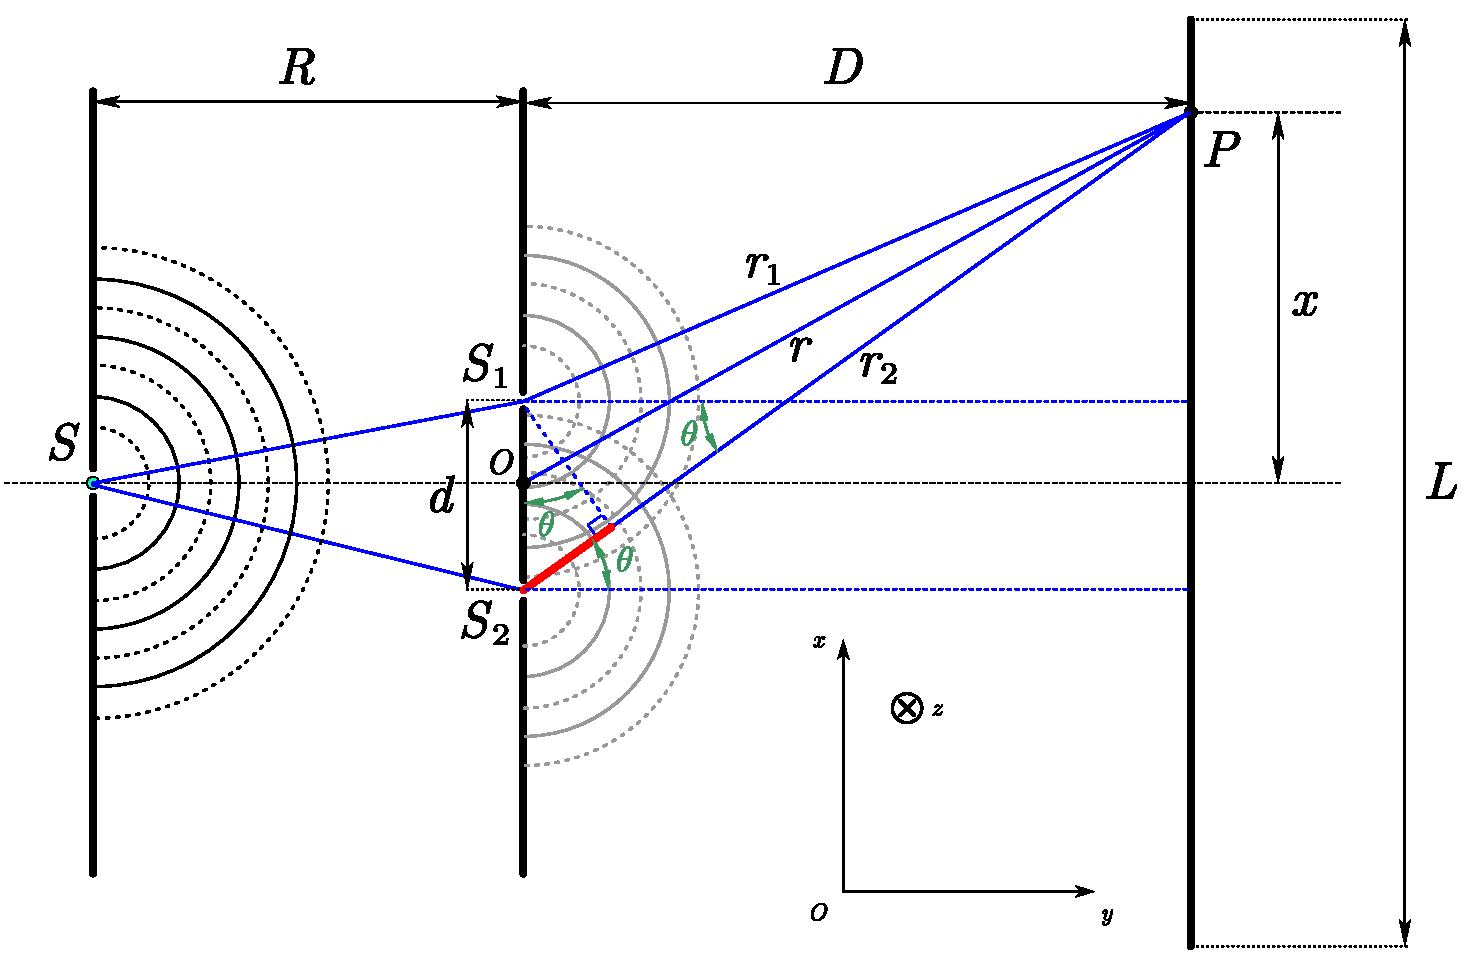
\includegraphics[height=160pt]{assets/3/杨双.pdf}
        \caption{ 杨氏双缝干涉装置 }
    \end{subfigure}\begin{subfigure}[t]{0.48\columnwidth}\centering
        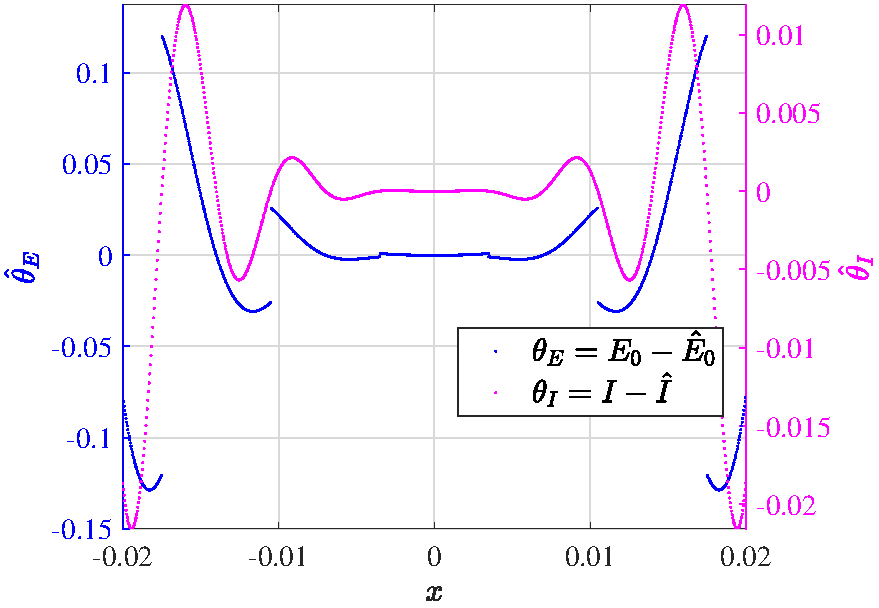
\includegraphics[height=160pt]{assets/3/杨残差.pdf}
        \caption{ 近似模型残差分布 }
    \end{subfigure}
    \caption{ 杨氏双缝干涉装置与近似模型残差分布 }\label{杨氏双缝干涉装置}
\end{figure}


设通过双缝屏后,两柱面波的振幅系数相同,都为 $A$,真空介电常量 $\varepsilon_0 = 8.854187817 \times 10^{-12}\ \mathrm{F\cdot m^{-1}}$,真空磁导率 $\mu_0 = 4\pi \times 10^{-7}\ \mathrm{N\cdot A^{-2}}$,则两波的光强度分别为
\begin{equation}
    I_1 = \frac{1}{2}\sqrt{\frac{\varepsilon_0}{\mu_0}}E_{1,0}^2 = \frac{1}{2}\sqrt{\frac{\varepsilon_0}{\mu_0}} \cdot \frac{A^2}{r_1},\quad
    I_2 = \frac{1}{2}\sqrt{\frac{\varepsilon_0}{\mu_0}} \cdot \frac{A^2}{r_2}
\end{equation}
那么,接受屏上的振幅和强度分布为:
\begin{equation}
    E_0 = A \sqrt{ \frac{1}{r_1} + \frac{1}{r_2} + \frac{2}{\sqrt{r_1r_2}} \cos \left( \frac{2 \pi}{\lambda}(r_1 - r_2) \right)  }  ,\quad 
    I = A^2\sqrt{\frac{\varepsilon_0}{\mu_0}}\left[ \frac{1}{2}\left( \frac{1}{r_1} + \frac{1}{r_2} \right) + \frac{\cos \left( \frac{2 \pi}{\lambda}(r_1 - r_2) \right)}{\sqrt{r_1r_2} } \right]
\end{equation}
装置参数在典型值附近时,可以有近似:
\begin{equation}\label{杨氏双缝干涉近似}
\frac{r_1}{D} = \frac{r_2}{D} = 1,\quad r_2 - r_1 = \frac{d}{\sin \theta} = \frac{d}{\sin \theta} = \frac{x d}{ D },\quad I_1 = I_2
\end{equation}
得到近似后的振幅和强度分布如下,其中 ${\color{red} \Delta x= \frac{D}{d}\lambda }$ 称为条纹间距。
\begin{gather}\label{杨氏双缝干涉近似结果}
    E_0(x) = \frac{\sqrt{2}A}{\sqrt{D}} \cdot \sqrt{1 + \cos \left( \frac{2 \pi d}{\lambda D}x \right)} = \frac{\sqrt{2}A}{\sqrt{D}} \cdot \sqrt{1 + \cos \left( \frac{2 \pi x}{\Delta x} \right)} \\ 
    I(x) = \sqrt{\frac{\varepsilon_0}{\mu_0}} \cdot \frac{A^2}{D} \left[ 1 + \cos \left( \frac{2 \pi  d}{\lambda D }x \right) \right] = \sqrt{\frac{\varepsilon_0}{\mu_0}} \cdot \frac{A^2}{D} \left[ 1 + \cos \left( \frac{2 \pi x}{\Delta x} \right) \right]
\end{gather}


图 \ref{近似模型与非近似模型的比较}\footnote{图 \ref{杨氏双缝干涉装置} (b) 与图 \ref{近似模型与非近似模型的比较} 源码见附录 \ref{杨氏双缝干涉装置 源码}} 展示了未近似和近似时,振幅、光强在接受屏上的分布情况,图 \ref{杨氏双缝干涉装置} (b) 是近似与未近似模型的残差分布,其中装置参数采取典型值。计算得到一些误差参数(对横坐标均匀离散 1000 个点)如下\footnote{这些误差参数的定义详见 \href{https://yidingg.github.io/YiDingg/\#/Notes/Else/GoodnessOfFit}{YiDingg > Notes > Else > Goodness of Fit}}: 
\begin{gather}
\begin{aligned}
    &1 - R^2_{E_0} = 0.0000030505,              && 1 - R^2_{I} = 0.0000024290 \\
    &1 - R^2_{\text{adj}, E_0} = 0.0000030536,  && 1 - R^2_{\text{adj}, I} = 0.0000024314 \\
    & MAPE_{E_0}  = 0.0020522069, && MAPE_{I}  = 0.00415721554 \\
    & MyMAPE_{E_0}  = 0.0017294036, && MyMAPE_{I}  = 0.0010723717 \\
    & RMSE_{E_0}  = 0.0534542000, && RMSE_{I}  = 0.0071984799 \\
    & fitness_{\text{adj}, E_0}  = 0.0534543632, && fitness_{\text{adj}, I}  = 0.0071984975 \\
    & SAAE_{E_0}  = 0.0005185186, && SAAE_{I}  = 0.0006493885
\end{aligned}
\end{gather}

%\begin{gather}
%\begin{matrix}
%    \text{相对平均值误差:} \text{RME}_{E_0} =  0.0001336621,\quad \text{RME}_{I} = 0.0002192205 \\
%    \text{决定系数:} \text{R}^2_{E_0} =  0.9999969495,\quad \text{R}^2_{I} = 0.9999975710 \\
%    \text{调整决定系数:} \text{R}^2_{\text{adj}, E_0} = 0.9999969464,\quad \text{R}^2_{\text{adj}, I} = 0.9999975686 \\
%    \text{平均标准绝对残差:} \text{RS}_{E_0} = 0.0005191648,\quad \text{RS}_{I} = 0.0006515739\\
%    \text{平均标准平方残差:} \text{RSS}_{E_0} = 0.0000007426 ,\quad \text{RSS}_{I} = 0.0000012850  \\ 
%    \text{标准面积误差:} \text{SAE}_{E_0} = 0.0005185186 ,\quad \text{SAE}_{I} = 0.0006493885
%\end{matrix}
%\end{gather}


由图 \ref{杨氏双缝干涉装置} (b),图 \ref{近似模型与非近似模型的比较} 和列出的误差参数可以看到,近似效果很好。

\begin{figure}[H]\centering
\begin{subfigure}[t]{0.5\columnwidth}\centering
    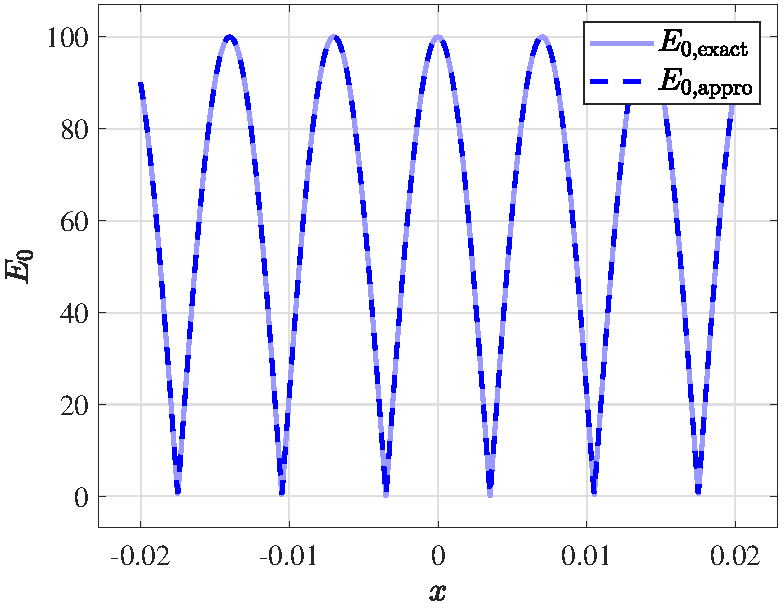
\includegraphics[height=165pt]{assets/3/杨电场.pdf}
    \caption{ 电场振幅位置分布 }
\end{subfigure}\hfill
\begin{subfigure}[t]{0.5\columnwidth}\centering
    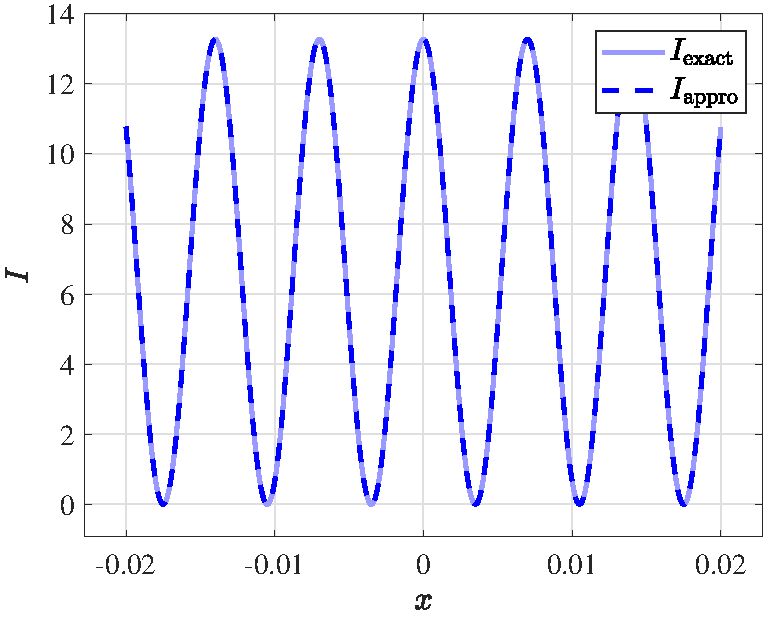
\includegraphics[height=165pt]{assets/3/杨光强.pdf}
    \caption{ 光强位置分布 }
\end{subfigure}
\caption{ 近似模型与非近似模型的比较 }\label{近似模型与非近似模型的比较}
\end{figure}

\noindent 杨氏双缝干涉的特点:
\begin{enumerate}
\item 非定域干涉:在干涉场中离双孔不太近也不太远的区域处处有干涉
\item 自相干:相干光波来自同一波源
\item 定态干涉:振幅(或强度)在干涉场中的分布仅与位置有关,与时间无关
\end{enumerate}


白光光源与其他补充内容详见 \href{https://produckthieves.home.blog/2020/02/10/phy-c15-double-slit-interference/}{PHY C15: Double Slit Interference}、\href{https://www.physics.louisville.edu/cldavis/phys299/notes/lo_interference.html}{University of Louisville: Double Slit Interference} 以及 \href{https://zhuanlan.zhihu.com/p/335815195}{知乎:双缝干涉实验},我们不多赘述。从另一个角度,也可以利用双曲线的定义杨氏干涉的精确模型 + 近似模型,详见 \href{https://www.zhihu.com/question/382600481/answer/2565939868}{知乎:杨氏干涉的条纹间距}。

\subsection{杨氏实验中光源位置和宽度对干涉条纹的影响}\label{杨氏实验中光源位置和宽度对干涉条纹的影响}

为提高分析效率,此节的推导都采用近似模型。接受屏上相邻明(暗)条纹的间距 $\Delta x$ 为:
\begin{equation}
\Delta x = \frac{D \lambda}{d}
\end{equation}
取 $\lambda = 700.0\ \mathrm{nm}$ 的红光,$\Delta x = 7 \ \mathrm{mm}$,可被人眼分辨。称 $\frac{\Delta x}{2}$ 为条纹宽度,此时条纹宽度为 $3.5\ \mathrm{mm}$。

下面依次讨论光源位置、光源宽度对干涉条纹的影响。先考虑理想点光源的微小移动引起的干涉条纹移动。当点光源位于中轴线上时,0 级明纹也在轴上,假设光源 S 向下移动距离 $ \delta_s > 0$,也即向上移动 $(-\delta_s)$,在近似条件 \ref{杨氏双缝干涉近似} 下,以及 $R \gg d$ 时近似有 $R_1 - R_2 = \frac{d(-\delta_s)}{R}$,得到 0 级明纹向上移动的距离 $\delta_x$ 如下,其中负号表示两者移动方向相反。
\begin{equation}
\delta_x = - \frac{D}{R}\delta_s
\end{equation}

实际光源并非是理想的点光源,而是有一定的光源宽度,虽然对干涉条纹位置影响不大,但会对条纹对比度产生明显的影响。理想点光源不在中央时,屏幕上的强度分布大小可以近似不变,仅是发生上下平移。记点光源位置为 $\delta_s$,在公式 \ref{杨氏双缝干涉近似结果} 中作映射 $x \longrightarrow x - \delta_x$,并简记接受屏上的最大光强为 $I_{\text{max}} = 2 \frac{\varepsilon_0}{\mu_0} \cdot \frac{A^2}{r}$,简记 $x$ 前的系数为 $\eta = \frac{2 \pi}{\Delta x}$,得到新的强度分布:
\begin{align}
I(x) &= \frac{I_{\text{max}}}{2}\left[
1 + \cos \left( \eta (x - \delta_x)\right)
\right] = \frac{I_{\text{max}}}{2}\left[
    1 + \cos \left( \eta x + \eta\frac{D}{R}\delta_s\right)
    \right]
\\
= &
\frac{I_{\text{max}}}{2}\left[
1 + \cos \left( \eta x \right)\cos \left(\eta\frac{D}{R}\delta_s \right) - \sin \left( \eta x \right)\sin \left( \eta\frac{D}{R}\delta_s \right)
\right],\quad \eta = \frac{2 \pi}{\Delta x}
\end{align}
设光源在中央且宽度为 $b$(即发光区域在 $[-\frac{2}{b},\ \frac{2}{b}]$),光源均匀发光(事实上这个条件比较苛刻,现实中的激光器无法做到,需要对光线进行处理),屏幕上的强度分布 $I(x, b)$ 和条纹对比度为:
\begin{gather}
I(x, b) = \frac{I_{\text{max}}}{2b} \int_{-\frac{b}{2}}^{\frac{b}{2}} \left[ 1 + \cos \left( \eta x \right)\cos \left( \eta\frac{D}{R}\delta_s \right) - \sin \left( \eta x \right)\sin \left( \eta\frac{D}{R}\delta_s \right) \right] \mathrm{d} \delta_s 
\\ 
= \frac{I_{\text{max}}}{2} \left[ 1 + \frac{\sin \left( \frac{\eta D}{2 R} b \right)}{\frac{\eta D}{2 R} b}\cdot \cos \left( \eta x \right) \right] 
= \frac{I_{\text{max}}}{2} \left[ 1 + \sinc \left(\frac{\pi d}{\lambda R} b\right) \cdot \cos \left( \frac{2 \pi x}{\Delta x}  \right) \right] 
\\ 
\gamma = \gamma(b) 
= \left| \frac{\sin \left( \frac{\pi d}{\lambda R} b \right)}{\frac{\pi d}{\lambda R} b} \right|
= \left| \sinc \left(\frac{\pi d}{\lambda R} b\right) \right|
\end{gather}
强度分布 $I(x, b)$ 与干涉条纹对比度 $\gamma(b)$ 如图 \ref{光源宽度} 所示\footnote{源码见附录 \ref{光源宽度 源码}},当 $b = \frac{\lambda R}{d}$ 时,条纹对比度第一次为 0,称为光源极限宽度 $b_0$,此时认为光源完全不相干。总之,对任意的光源线度 $b$ 和双缝间距 $d$,有限制 $bd <  \lambda R$。

\begin{figure}[H]\centering
\begin{subfigure}[t]{0.5\columnwidth}\centering
    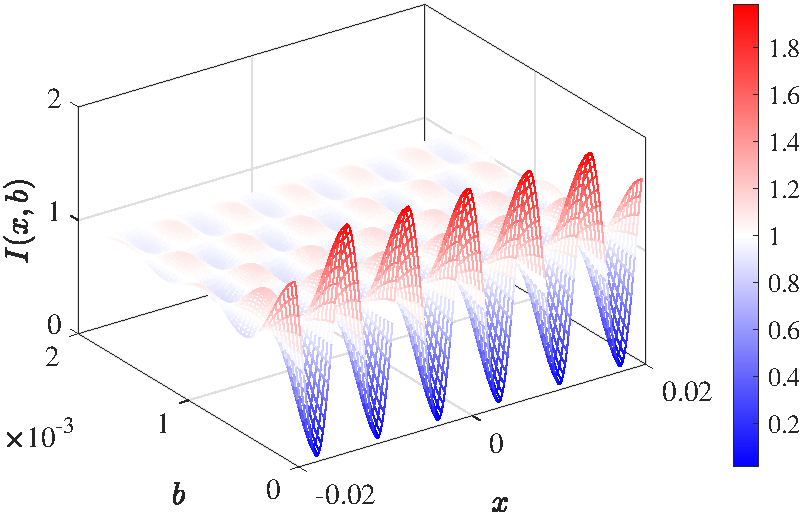
\includegraphics[height=160pt]{assets/3/光强分布.pdf}
    \caption{ 光强分布随光源宽度的变化 }
\end{subfigure}\hfill
\begin{subfigure}[t]{0.5\columnwidth}\centering
    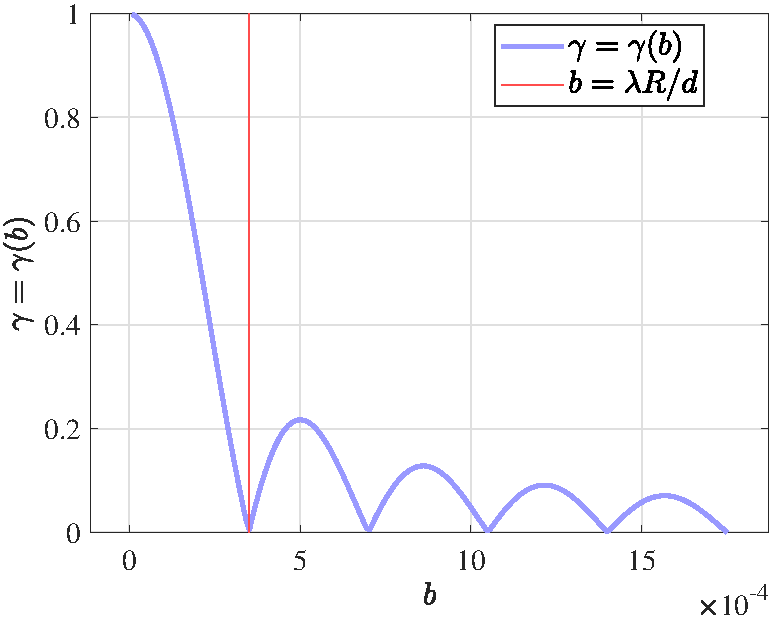
\includegraphics[height=160pt]{assets/3/干涉条纹对比度.pdf}
    \caption{ 干涉条纹对比度随光源宽度的变化 }
\end{subfigure}
\caption{ 光源宽度对干涉条纹的影响 }\label{光源宽度}
\end{figure}

\section{分振幅干涉}

\subsection{多光束薄膜干涉}\label{多光束薄膜干涉}

%\begin{table}[H]\centering
%    %\renewcommand{\arraystretch}{1.5} % 调整行间距为 1.5 倍
%    %\setlength{\tabcolsep}{1.5mm} % 调整列间距
%    \caption{\textbf{薄膜干涉光线的相位}}
%    \label{薄膜干涉光线的相位}
%\begin{tabular}{cccccccccc}\toprule
%    序号 & 0 & 1 & 2 & 3 & 4  \\
%    \midrule
%    $A$ 光 $s$ 波相位 & 0 & 1 & 2 & 3 & 4  \\
%    $A$ 光 $p$ 波相位 & - & 1 & 2 & 3 & 4  \\
%    $B$ 光 $s$ 波相位 & 0 & 1 & 2 & 3 & 4  \\
%    $B$ 光 $p$ 波相位 & - & 1 & 2 & 3 & 4  \\
%    \bottomrule
%\end{tabular}
%\end{table}



如图 \ref{薄膜干涉} (a) 所示,一入射光接近垂直入射到一薄膜时($\theta_i < \theta_B$),发生多次反射、透射,下面讨论其能量与干涉情况。

\begin{figure}[H]\centering
    \begin{subfigure}[t]{0.6\columnwidth}\centering
        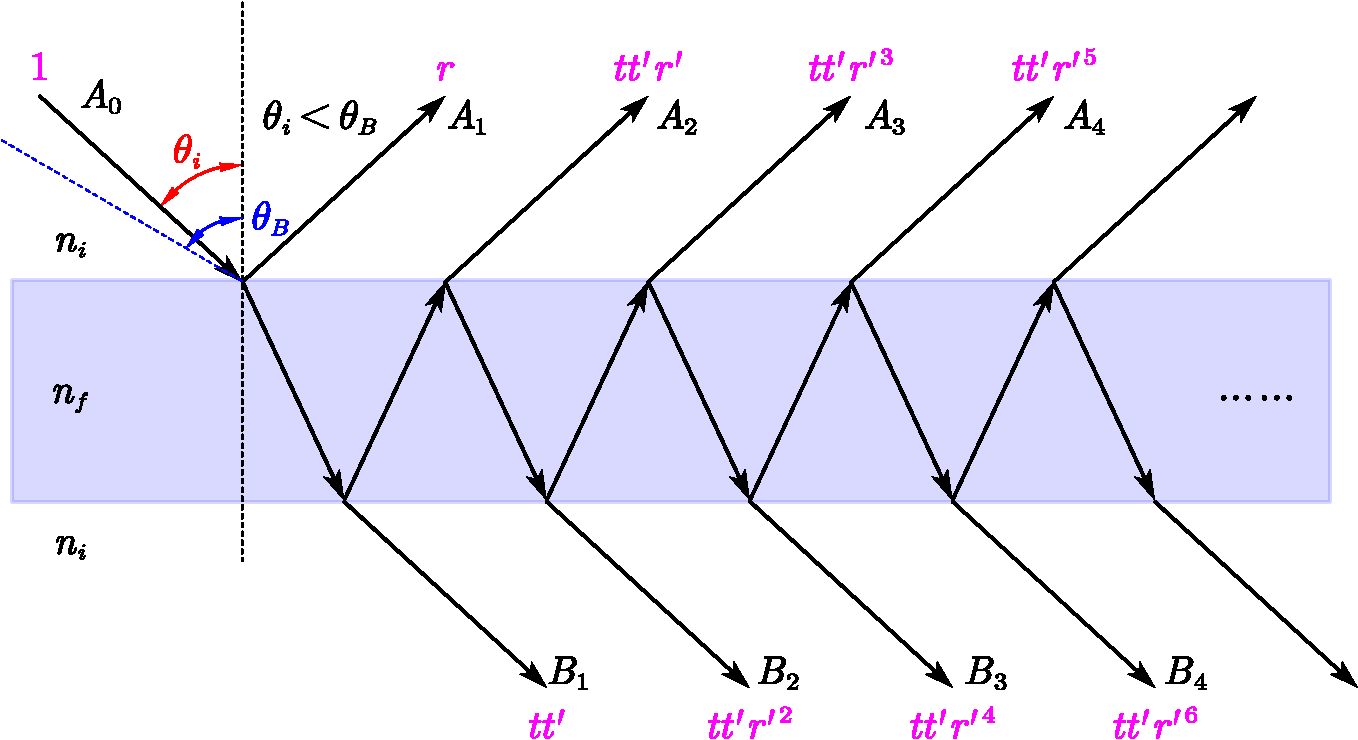
\includegraphics[height=145pt]{assets/3/薄膜干涉.pdf}
        \caption{ 薄膜多光束干涉 }
    \end{subfigure}\hfill
    \begin{subfigure}[t]{0.4\columnwidth}\centering
        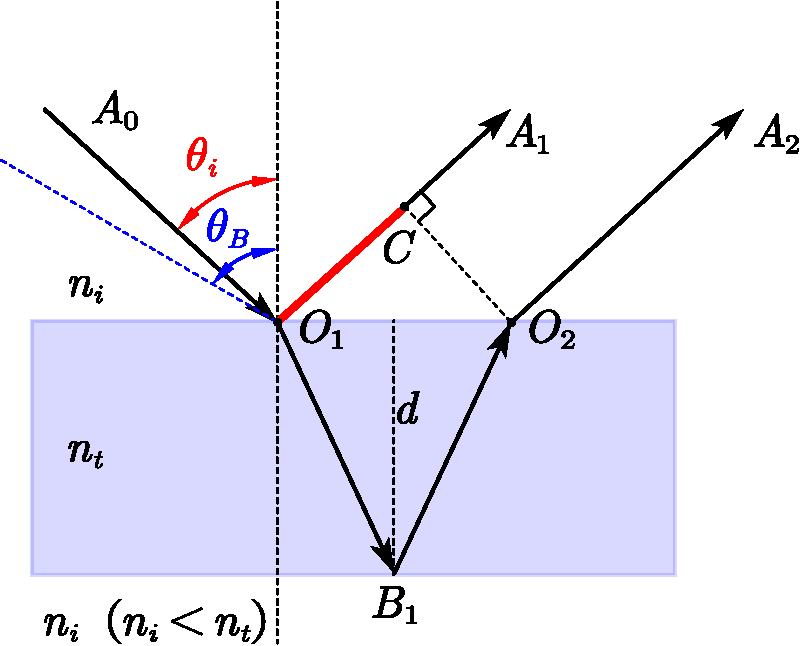
\includegraphics[height=145pt]{assets/3/薄膜双光束干涉.pdf}
        \caption{ 薄膜双光束干涉 }
    \end{subfigure}
    \caption{ 薄膜干涉 }\label{薄膜干涉}
\end{figure}

由于没有发生全反射,相位变化是平凡的(透射无相变,反射只能是 $-\pi$ 或零),而反射光的相位变化已经包含在振幅反射系数 $r$ 中了(由其正负表示)。因此,在分析多光束干涉时,只需考虑各光(有正负)的振幅以及光程差,处理波函数的表达式的叠加即可。

记相邻两束反射(透射)光的光程差为 $\Delta l$,光程差带来的相位差为 $\delta$({\color{red} 无需考虑反射相位突变,因为它涵盖在了振幅的正负中}),由图 \ref{薄膜干涉} (b) 所示,可求得:
\begin{gather}
    \Delta l = l_2 - l_1 = 2 n_f\cdot  \overline{O_1B_1} - n_i\cdot  \overline{O_1 C} = \frac{2 n_f d}{\cos \theta_f} - 2 n_i \sin \theta_i \tan \theta_f d = 2 n_f d \cos \theta_f \\ 
    \delta = \frac{2 \pi}{\lambda_i} \Delta l = \frac{4 \pi n_f d \cos \theta_f}{\lambda_i}
\end{gather}
由公式 \ref{斯托克斯倒逆关系}(斯托克斯倒逆关系),$r + r' = 1,\ tt' + rr' =1$,结合等比数列极限($n \to \infty$),可得反射波的总振幅系数 $r_A$、透射波的总振幅系数 $t_B$:
\begin{gather}
    r_A 
    = r + tt'r' e^{i \delta}\left( 1 + r'^2e^{i \delta} +  r'^4e^{2 i \delta} + \cdots\right) 
    = r +  \frac{tt'r'e^{i \delta}}{1 - r'^2e^{i \delta}} 
    = r \left( \frac{1 - e^{i \delta}}{1 - r^2 e^{i \delta}} \right)
    \\ 
    t_B 
    =  tt' \left( 1 + r'^2e^{i \delta} +  r'^4e^{2 i \delta} + \cdots \right) = \frac{tt'}{1 - r'^2e^{i \delta}} = \frac{1 - r^2}{1 - r^2 e^{i \delta}}
\end{gather}

由于上述推导与角标 $s$ 或 $p$ 无关,因此对 $s$ 波和 $p$ 波都成立。

也即得到:
\begin{gather}
    r_{A,s}= \frac{\boldsymbol{E_{r,s}}}{\boldsymbol{E_{i,s}}} = r_s \left( \frac{1 - e^{i \delta}}{1 - r_s^2 e^{i \delta}} \right),\quad 
    r_{B,p} = \frac{\boldsymbol{E_{r,p}}}{\boldsymbol{E_{i,p}}} = r_p \left( \frac{1 - e^{i \delta}}{1 - r_p^2 e^{i \delta}} \right) \\
    t_{B,s} = \frac{\boldsymbol{E_{t,s}}}{\boldsymbol{E_{i,s}}} = \frac{1 - r_s^2}{1 - r_s^2 e^{i \delta}} ,\quad
    t_{B,p} = \frac{\boldsymbol{E_{t,p}}}{\boldsymbol{E_{i,p}}} = \frac{1 - r_p^2}{1 - r_p^2 e^{i \delta}}
\end{gather}
据此,可以定义光学经过薄膜时的能量系数 $R_{F-P,s},\ R_{F-P,p},\  T_{F-P,s},\  T_{F-P,p}$(与菲涅尔公式中的能量系数类似,但物理意义不同):
\begin{gather}
    R_{F-P,s} = |r_{A,s}|^2 = \frac{4 R_s \sin^2 \frac{\delta}{2}}{(1 - R_s)^2}, \quad 
    R_{F-P,p} = |r_{A,p}|^2 = \frac{4 R_p \sin^2 \frac{\delta}{2}}{(1 - R_p)^2} \\ 
    T_{F-P,s}= \frac{n_1 \cos \theta_1}{n_3 \cos \theta_3} |t_{B,s}|^2 = \frac{(1 - R_s)^2}{ (1 - R_s\cos \delta)^2 + R_s^2 \sin^2 \delta} \\
    T_{F-P,p} = \frac{n_1 \cos \theta_1}{n_3 \cos \theta_3} |t_{B,p}|^2 = \frac{(1 - R_p)^2}{ (1 - R_p\cos \delta)^2 + R_p^2 \sin^2 \delta}
\end{gather}
其中 $\theta_1 = \theta_3 = \theta_i,\ n_1 = n_3 = n_i$。角标 $F-P$ 指 Fabry-Perot Interferometer(法布里-珀罗干涉仪),是一种利用薄膜产生干涉现象的仪器。定义 $F_s = \frac{4R_s}{(1 - R_s)^2},\ F_p = \frac{4R_p}{(1 - R_p)^2}$,称为精细度,则上式可简写为:
\begin{gather}
    R_{F-P, s} = \frac{F_s \sin^2 \frac{\delta}{2}}{1 + F_s \sin^2 \frac{\delta}{2}},\quad R_{F-P, p} = \frac{F_p \sin^2 \frac{\delta}{2}}{1 + F_p \sin^2 \frac{\delta}{2}} \\
    T_{F-P, s} = \frac{1}{1 + F_s \sin^2 \frac{\delta}{2}},\quad T_{F-P, p} = \frac{1}{1 + F_p \sin^2 \frac{\delta}{2}}\\ 
    \delta = \frac{4 \pi n_f d \cos \theta_f}{\lambda_i},\quad F_s = \frac{4R_s}{(1 - R_s)^2},\quad F_p = \frac{4R_p}{(1 - R_p)^2}
\end{gather}
其中 $n_f$ 是薄膜的折射率,容易验证上式满足能量守恒。在实际操作中,基本都会选取接近垂直的入射光,此时 $s$ 波 $p$ 波(近似)具有相同的能量系数 $R = R_s = R_p$,因此又常写为下面的式子:
\begin{gather}
    R_{F-P} = \frac{F \sin^2 \frac{\delta}{2}}{1 + F \sin^2 \frac{\delta}{2}},\quad T_{F-P} = \frac{1}{1 + F \sin^2 \frac{\delta}{2}},\quad F = \frac{4R}{(1 - R)^2},\quad \delta = \frac{4 \pi n_f d \cos \theta_f}{\lambda_i}
\end{gather}

$T_{F-P} = T_{F-P}(F, \delta)$ 的图像如下所示\footnote{源码见附录 \ref{精细度对透射率的影响 源码}},$F$ 越大,透射光的对比度越高,在干涉现象中形成的条纹越明显,且 $F$ 增大时,透射峰的宽度减小,亮条纹变细变锐利。

\begin{figure}[H]\centering
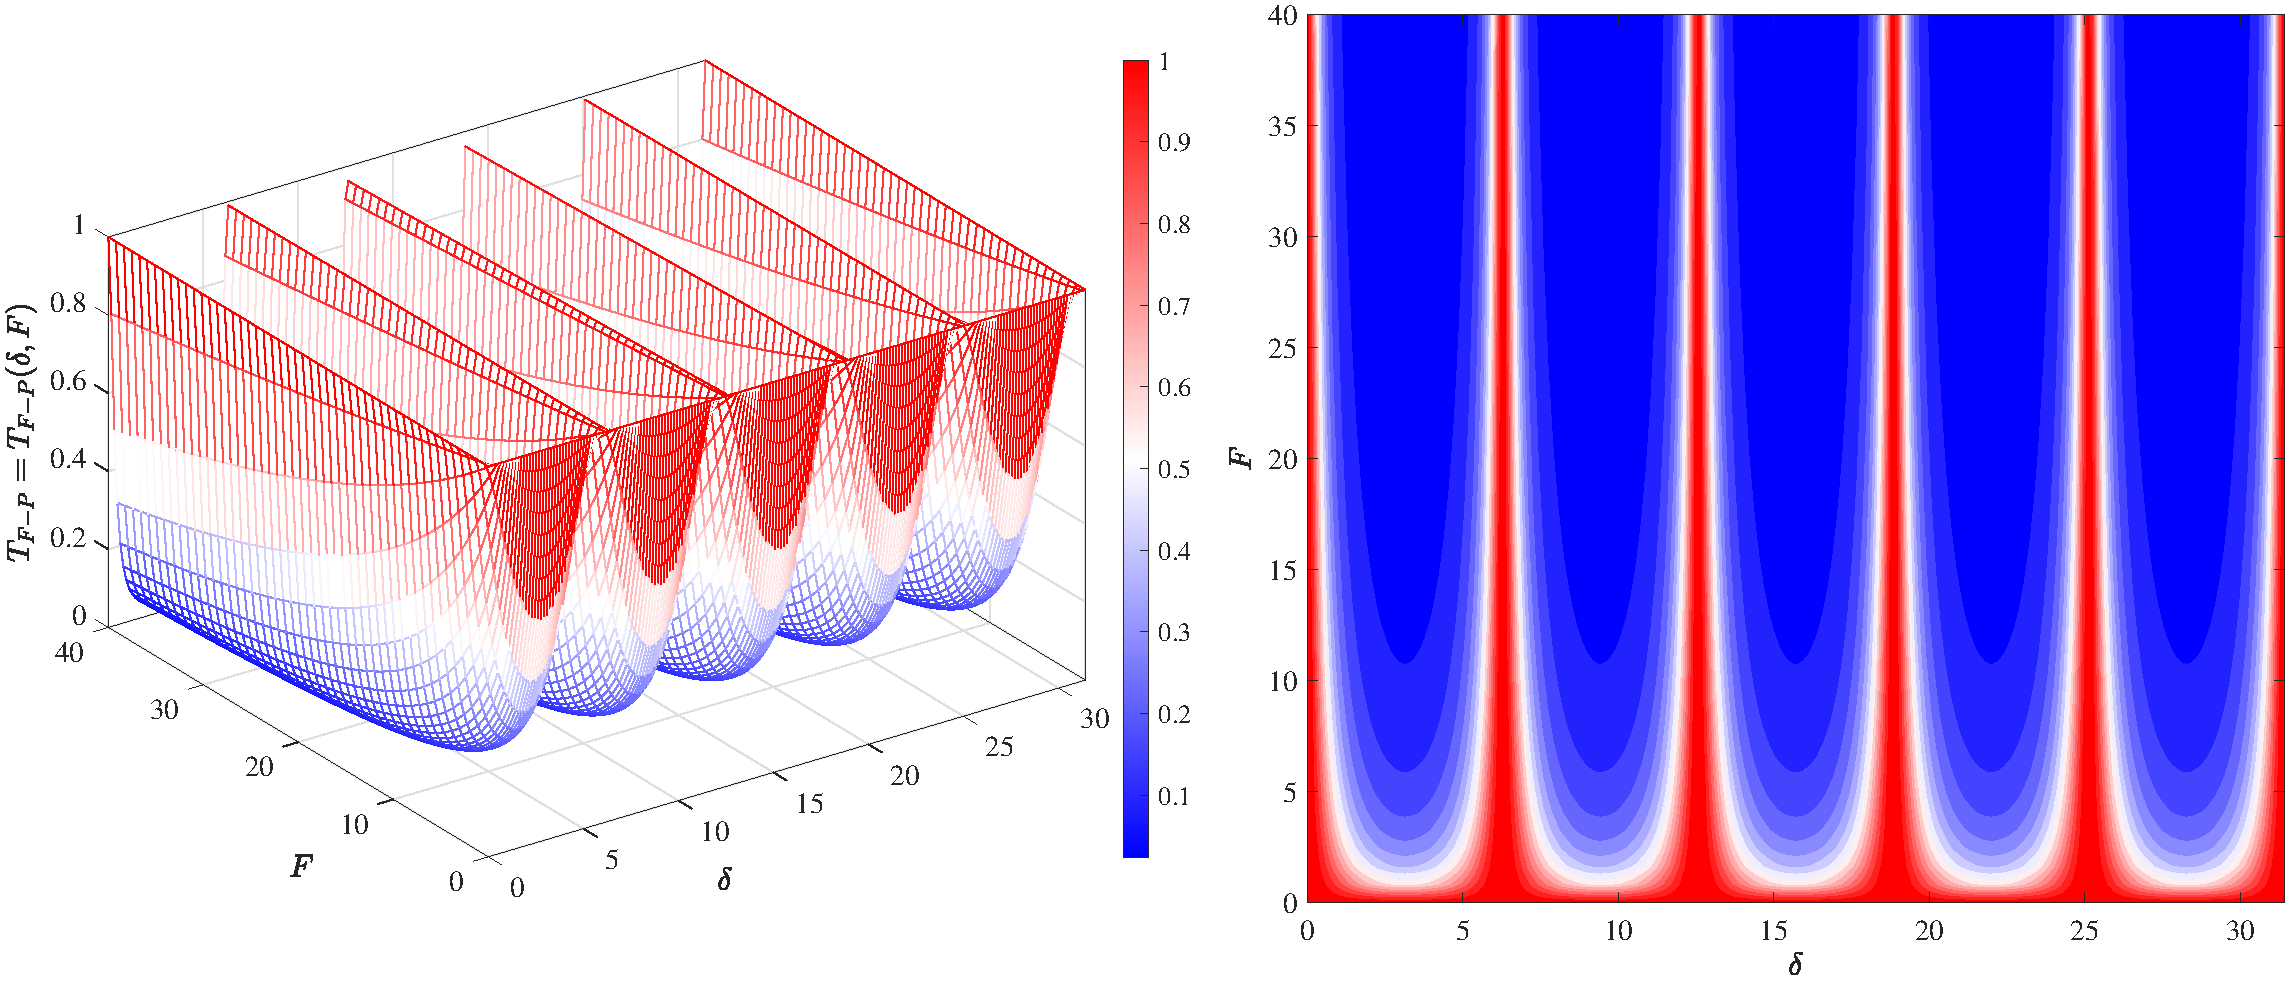
\includegraphics[width=\columnwidth]{assets/3/精细度对透射率的影响.pdf}
\caption{ 精细度对透射率的影响}\label{精细度对透射率的影响}
\end{figure}

实际中常基于上面理论,设计出增透膜、增反膜等薄膜,实现光的选择性透射、反射。如果遇到,直接利用反射相位突变进行分析即可。

更多有关多光束薄膜干涉(法布里-珀罗干涉仪 Fabry-Perot Interferometer)的内容见 \href{https://zhuanlan.zhihu.com/p/579184206}{知乎: Fabry-Perot Interferometer},以及 \href{https://zhuanlan.zhihu.com/p/453978087}{知乎: F-P干涉仪}。

%不妨设入射光相位为 0,强度为 1,依据公式 \ref{对称前后的振幅与能量系数%变化},在图中标出各光线的强度。$n_i < n_f$ 时,它们的相位如表 \ref{薄%膜干涉光线的相位1} 所示,$n_i > n_f$ 时,各光线相位如表 \ref{薄膜干涉%光线的相位2} 所示,其中“$A$ $s$” 指 $A$ 光 $s$ 分量的相位。

%\begin{center}\noindent\begin{minipage}{0.5\columnwidth}
%    \noindent\begin{table}[H]\centering
%        %\renewcommand{\arraystretch}{1.5} % 调整行间距为 1.5 倍
%        %\setlength{\tabcolsep}{1.5mm} % 调整列间距
%        \caption{\textbf{薄膜干涉光线的相位 $(n_i < n_f)$}}
%        \label{薄膜干涉光线的相位1}
%    \begin{tabular}{|c|c|c|c|c|c|c|c|c|c|}\hline
%        序号 & $A$ $s$ & $A$ $p$  & $B$ $s$& $B$ $p$ \\
%        \hline
%        0 & 0       & 0      &   -     & -  \\
%        1 & 0       & $-\pi$ &   0     & 0  \\
%        2 & $-\pi$  & 0      & $-2\pi$ & 0  \\
%        3 & $-3\pi$ & 0      & $-4\pi$ & 0  \\
%        4 & $-5\pi$ & 0      & $-6\pi$ & 0  \\
%        \hline
%    \end{tabular}
%    \end{table}
%\end{minipage}\hfill\begin{minipage}{0.5\columnwidth}
%    \noindent\begin{table}[H]\centering
%        %\renewcommand{\arraystretch}{1.5} % 调整行间距为 1.5 倍
%        %\setlength{\tabcolsep}{1.5mm} % 调整列间距
%        \caption{\textbf{薄膜干涉光线的相位 $(n_i > n_f)$}}
%        \label{薄膜干涉光线的相位2}
%    \begin{tabular}{|c|c|c|c|c|c|c|c|c|c|}\hline
%        序号 & $A$ $s$ & $A$ $p$  & $B$ $s$& $B$ $p$ \\
%        \hline
%        0 & 0      & 0       & - &   -      \\
%        1 & $-\pi$ & 0       & 0 &   0      \\
%        2 & 0      & $-\pi$  & 0 & $-2\pi$  \\
%        3 & 0      & $-3\pi$ & 0 & $-4\pi$  \\
%        4 & 0      & $-5\pi$ & 0 & $-6\pi$  \\
%        \hline
%    \end{tabular}
%    \end{table}
%\end{minipage}\end{center}

\subsection{双光束薄膜干涉}

当振幅反射率 $r$ 较小时,$A$ 光的振幅衰减很快,可以仅考虑双光束干涉($A_1$ 与 $A_2$),而忽略剩余反射光带来的影响,如图 \ref{薄膜干涉} (b)。实际操作中,也常用薄透镜将两束出射光汇聚于一点,而不会引起附加的相位差。反射后光线 $O_1A_1$ 与 $O_2A_2$ 的光程差 $\Delta l$ 为:
\begin{equation}
    \Delta l = l_2 - l_1 = 2 n_f\cdot  \overline{O_1B_1} - n_i\cdot  \overline{O_1 C} = \frac{2 n_f d}{\cos \theta_t} - 2 n_i \sin \theta_i \tan \theta_t d = 2 n_f d \cos \theta_f
\end{equation}
即 $A_2$ 比 $A_1$ 多走了 $\Delta l$ 的光程,相当于相位增量 $ - \omega \frac{\Delta l}{c}$,算上反射时 $A_2$ 与 $A_1$ 之间的相位增量 $-\pi$(事实上 $s$ 波是 $-\pi$ 而 $p$ 波是 $\pi$),总光程差 OPD (Optical Path Difference, 常记为 $\Delta L$)($A_2$ 的减去 $A_1$)和总相位增量 $\Delta \alpha$ 为:
\begin{equation}
    \boxed{
        \Delta L = 2 n_f d \cos \theta_f + \frac{\lambda}{2}
    } ,\quad \Delta \alpha 
    = - \left(1 + \frac{4 n_f  \cos \theta_t}{\lambda} \cdot d \right) \pi
    = - \left[ 1 + \frac{4 n_f \sqrt{ 1 - \left(\frac{\sin \theta_i}{n_{ti}} \right)^2 }  }{\lambda} \cdot d \right] \pi
\end{equation}

随参数 $\theta_i$、$d$ 的改变,不同位置上会有不同的 $\Delta L$,得到不同的振幅大小,从而产生干涉条纹。

\subsection{等倾干涉}

\noindent 等倾干涉实验装置如图 \ref{等倾干涉实验装置} 所示,其干涉条纹特征为:
\begin{enumerate}
\item 亮条纹:$\Delta L = k \lambda \Longrightarrow \cos \theta_t = \frac{\lambda}{2 n_f d} \cdot (k - \frac{1}{2}),\quad k = 1, 2, 3, ... $
\item 暗条纹:$\Delta L = (k + \frac{1}{2}) \lambda \Longrightarrow \cos \theta_t = \frac{\lambda}{2 n_f d} \cdot k,\quad k = 0, 1, 2, 3, ... $
\item $r$ 较小时,等倾双光束强度近似相等,干涉条纹对比度接近 1
\item 称中心暗条纹为 0 级暗纹,往外依次是 1 级亮纹、1 级暗纹、2 级亮纹、2 级暗纹…… 
\item 等倾条纹{\color{red} 内疏外密}。这是因为:
\begin{gather}
\cos \theta_{t, n + 1} - \cos \theta_{t, n} = \frac{\lambda}{2 n_f d},\quad \frac{\cos \theta_{t, n + 1} - \cos \theta_{t, n} }{\theta_{t, n + 1} - \theta_{t, n}}\approx \frac{\mathrm{d} \cos \theta }{\mathrm{d} \theta } = - \sin \theta_n \\ 
\Longrightarrow \Delta r = (r_{n +1} - r_n) \propto (\theta_{t, n+1} - \theta_n) = - \frac{\lambda}{2d \sin \theta_{t, n}}
\end{gather}
随着 $r$ 的增大,入射光指在薄膜(半反射镜)上的点由中心向外移动,$\theta_i$ 增大,$\theta_t$增大,于是 $| \Delta r |$ 减小,条纹逐渐变密。
\item 增加薄膜厚度,条纹向外移动。薄膜厚度连续增大时,中心位置强度周期性变化,且不断生出新条纹向外移动,可以利用这一特点精确测量薄膜厚度的改变量。
\end{enumerate}

使用扩展光源(有宽度光源)时,条纹对比度不受影响,但条纹的强度增大,干涉图样更加明亮。

\begin{figure}[H]\centering
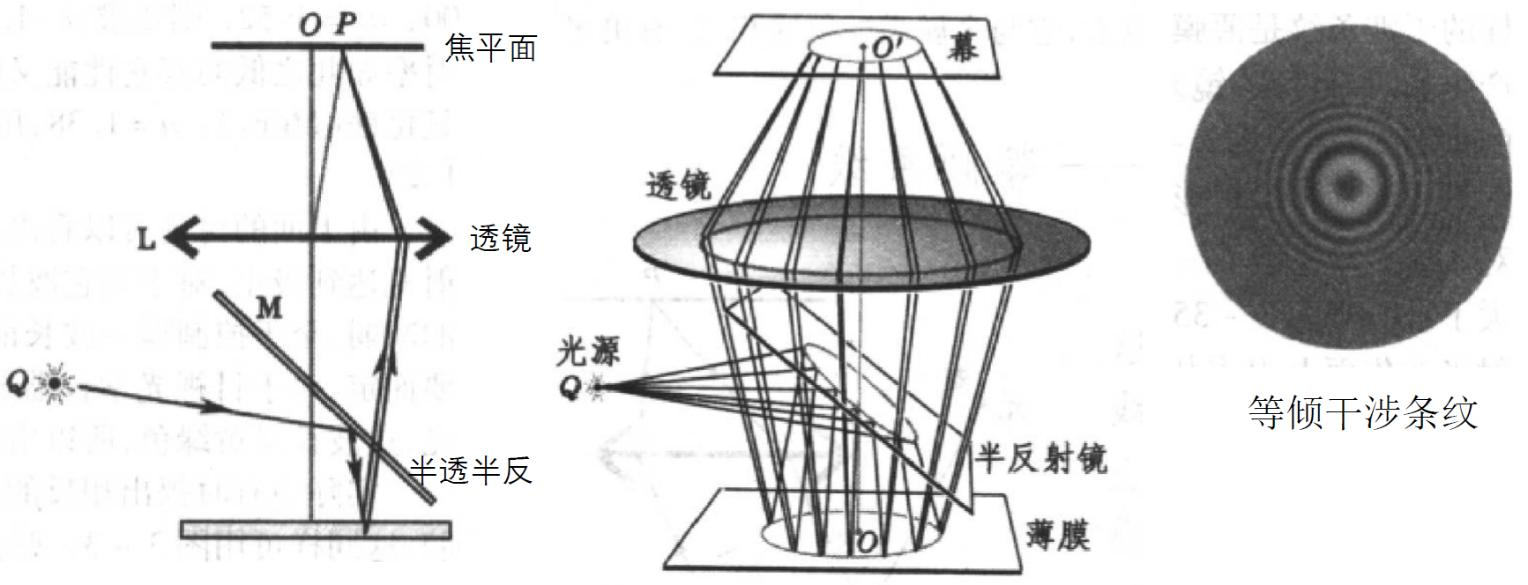
\includegraphics[width=0.7\columnwidth]{assets/3/等倾干涉.jpg}
\caption{ 等倾干涉实验装置}\label{等倾干涉实验装置}
\end{figure}

等倾干涉实验动图见链接 \href{https://www.123pan.com/s/0y0pTd-MgKj3}{https://www.123pan.com/s/0y0pTd-MgKj3}。

\subsection{等厚干涉} 

等厚干涉,也称等厚条纹干涉,是指由薄膜厚度不均匀而引起的干涉现象,它的主要变量(参数)是光学厚度 $n_f d$ 而不是 $\theta_i$(即 $\theta_t$)。等厚干涉产生的条纹一般是等厚位置的条纹,例如劈尖干涉、牛顿环等。

\subsubsection{劈尖干涉:}

两块(几乎)平行的玻璃板,夹角为 $\theta$ 极小,中间是空气层,即薄膜是空气,观察反射光的干涉现象。由 $R_{F-P} = \frac{ F \sin^2 (\frac{\delta}{2}) }{1 + F \sin^2 (\frac{\delta}{2})}$ 可知,明条纹对应 $\frac{\delta}{2} = (k + \frac{1}{2}) \pi$,这等价于 $2 n_f d\cos \theta_f + \frac{\lambda}{2} = k\lambda$,而暗条纹对应 $\frac{\delta}{2} = k \pi$。作近似 $n_f = 1$,$\cos \theta_f = 1$,得到:
\begin{gather}
    \text{明条纹:} d_k = \left( 1 + 2k \right)\cdot \frac{\lambda}{4},\quad \text{暗条纹:} d_k = \left( 2k \right)\cdot \frac{\lambda}{4},\quad k = 0, 1, 2, ... \\ 
    \text{条纹间距:}\Delta d = \frac{\lambda}{2},\quad \Delta x = \frac{\lambda}{2\sin \theta}
\end{gather}


可借此求出夹在玻璃板之间引起 $\theta$ 角的细小物体的直径。

\subsubsection{牛顿环:}

把一个曲率半径很大的凸透镜至于平面玻璃片上,两者接触的地方形成厚度不均匀的空气薄膜,得到的干涉条纹是一系列同心圆环。设凸透镜的半径为 $R$,以接触点为圆心 $O$,类似劈尖干涉中的近似,得到:
\begin{gather}
\text{明条纹:} r_k = \sqrt{\left(k + \frac{1}{2}\right)R\lambda} 
,\quad 
\text{暗条纹:} r_k = \sqrt{kR\lambda},\quad k = 0, 1, 2, ... 
\end{gather}

中心为 0 级暗纹,往外级数增大,干涉条纹逐渐变密。


\section{迈克尔逊干涉仪 (Michelson Interferometer)}

我们需要认识到,绝大多数的干涉现象,本质都是空间上两个(甚至多个)不同位置的球面波源(或其他类型的波)在某点的叠加。随着目标位置点 $P$ 的移动,发生叠加的两波(两束光)的 OPD(即 $\Delta L$)不断改变,得到不同的振幅大小,从而产生干涉图样。本节所介绍的几种干涉,其本质也是如此,只是具体实现方式不同。

\subsection{理想单色迈克尔逊干涉}

迈克尔逊干涉仪如图 \ref{迈克尔逊干涉仪} 所示,图中反射镜 $M_1$ 与 $M_2'$(虚镜)水平(此时的干涉现象类似等倾干涉),下方是接收屏或接受仪,图中的虚线光路表示出射向无穷远处(不被观察屏接收),或振幅较小而可以忽略的光线。

可以证明,从出射开始,分束所得到的两束光的空间光程差为 $\Delta l = 2 d \cos \theta$,其中 $\theta$ 是光束射向反射镜 $M$ 的入射角(光源平行出射时,$\theta = 0$)。再考虑上在分束镜 $G$ 处发生的相位突变(半波损失),与等倾干涉的结论类似,此时的条纹内疏外密,类似等倾干涉时的图 \ref{等倾干涉实验装置}。
\begin{align}
\begin{matrix}
\displaystyle \text{OPD: }& \Delta L = 2 d \cos \theta + \frac{\lambda}{2} \\ 
\displaystyle \text{亮条纹:}&\Delta L = k \lambda \Longrightarrow \cos \theta_k = \frac{\lambda}{2 n_f d} \cdot (k - \frac{1}{2}),\quad k = 1, 2, 3, ... \\ 
\displaystyle \text{暗条纹:}&\Delta L = (k + \frac{1}{2}) \lambda \Longrightarrow \cos \theta_k = \frac{\lambda}{2 n_f d} \cdot k,\quad k = 0, 1, 2, 3, ...\\ 
\displaystyle \text{条纹间距:}& | \Delta r | \propto  \frac{\lambda}{2d \sin \theta_k}
\end{matrix}
\end{align}


\begin{figure}[H]\centering
    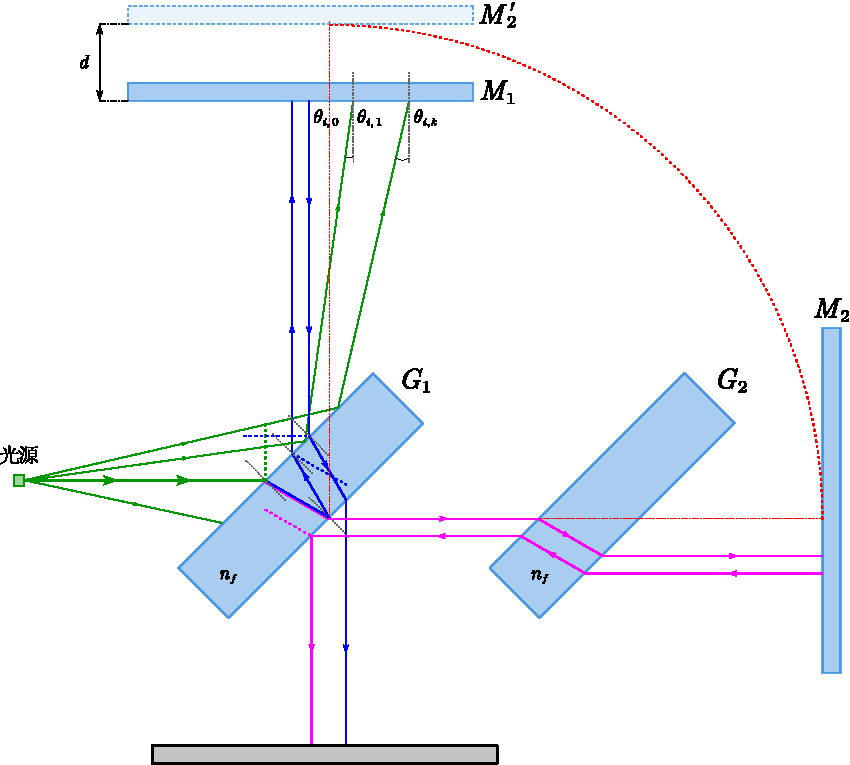
\includegraphics[width=0.8\columnwidth]{assets/3/迈克尔逊干涉仪.pdf}
    \caption{ 迈克尔逊干涉仪}\label{迈克尔逊干涉仪}
\end{figure}

对给定的第 $k$ 条亮纹,在图 \ref{迈克尔逊干涉仪} 的情况下($M_1$ 在 $M_2'$ 下方),将 $M_1$ 向上移动,$d$ 减小,$\cos \theta_k$ 增加,$\theta_k$ 减小,条纹向中心移动,直至完全收缩并消失。并且,随着 $d$ 越来越小,条纹间距 $| \Delta r |$ 越来越大,直至 $d \to 0$ 时 $| \Delta r | \to \infty$,中心条纹布满整个观察屏。继续向上移动 $M_1$,“穿过” $M_2'$ 后,干涉条纹重新出现。

记中心点($\theta_0 = 0$)处的条纹为中心(零号)条纹(它可能既不是极大值也不是极小值),对于给定的 $d$,得到与中心条纹相差 $\lambda$ 的第 $k$ 号条纹:
\begin{equation}
2d (1 - \cos \theta_k) = k \lambda \Longrightarrow \theta_k = \sqrt{\frac{k\lambda}{d}},\quad k = 0, 1, 2, 3, ... 
\end{equation}

关于如何将迈克尔逊干涉仪看作是具有两个不同位置波源的仪器,详见参考文献 \cite{Optics} Page 516,了解这一部分有助于我们理解干涉仪器的内涵。当 $M_1$ 与 $M_2'$ 不平行时,会发生类似等厚干涉的现象,出现平行直条纹。并且,从数学上可以证明,调整 $M_1$ 和 $M_2'$ 的方向,可以产生直线、圆、椭圆、抛物线或双曲线形的干涉条纹,这一部分我们不深究。

移动反射镜 $M_1$、$M_2$,或者在光路中插入其它介质,可以改变光程差,从而使干涉条纹发生移动。当光程差 $OPD$ 的改变量达到 $\lambda$ 时,每条干涉条纹都会移动一个条纹间距,移动到原先的相邻条纹处,这种方法可以用来测量镜面的微小移动距离,也可以测量插入介质的折射率。设镜面移动的距离或插入介质的厚度为 $\Delta d$,则有:
\begin{equation}
2n\Delta d = N\lambda_0
\end{equation}
其中 $n$ 是插入介质的折射率(移动镜面时相当于 $n=1$),$\lambda_0$ 是光源发出的光在空气中的波长,$N$ 是移动的条纹数。

\subsection{双色分立谱迈克尔逊干涉}\label{双色谱迈克尔逊干涉}

假设光源是双色光源,且两色的强度相同,对任意给定的 $\Delta L$(相当于给定位置 $P$),我们有:
\begin{gather}
I_1(\Delta L) = 2I_0 \left[1 + \cos \left(k_1 \Delta L\right)\right],\quad I_2(\Delta L) = 2I_0 \left[1 + \cos \left(k_2 \Delta L\right)\right] \\ 
\Longrightarrow I(\Delta L) = 4 I_0 \left[ 1 + \cos \left(\frac{\Delta k}{2}\Delta L\right)\cos(\overline{k} \Delta L) \right],\quad \Delta k = k_1 - k_2,\ \overline{k} = \frac{k_1 + k_2}{2} \\ 
\gamma = \gamma (\Delta L) = \left|\cos \left(\frac{1}{2}\Delta k \Delta L\right) \right|
\end{gather}
其中 $\Delta k$ 称为调制(空间角)频率,$\overline{k}$ 为平均(空间角)频率,$\Delta k \ll \overline{k}$ 时,可以观察到条纹对比度 $\gamma$ 随 $\Delta L$ 周期性变化,在 $\Delta L = \frac{1}{2} \frac{\lambda_0^2}{\Delta \lambda}$ 第一次下降到 0。

例如,$\lambda_1 = 550.0\ \mathrm{nm}$,$\lambda_2 = 600.0\ \mathrm{nm}$ 时的情况如图 \ref{双色光源的对比度分布情况} 所示。

\begin{figure}[H]\centering
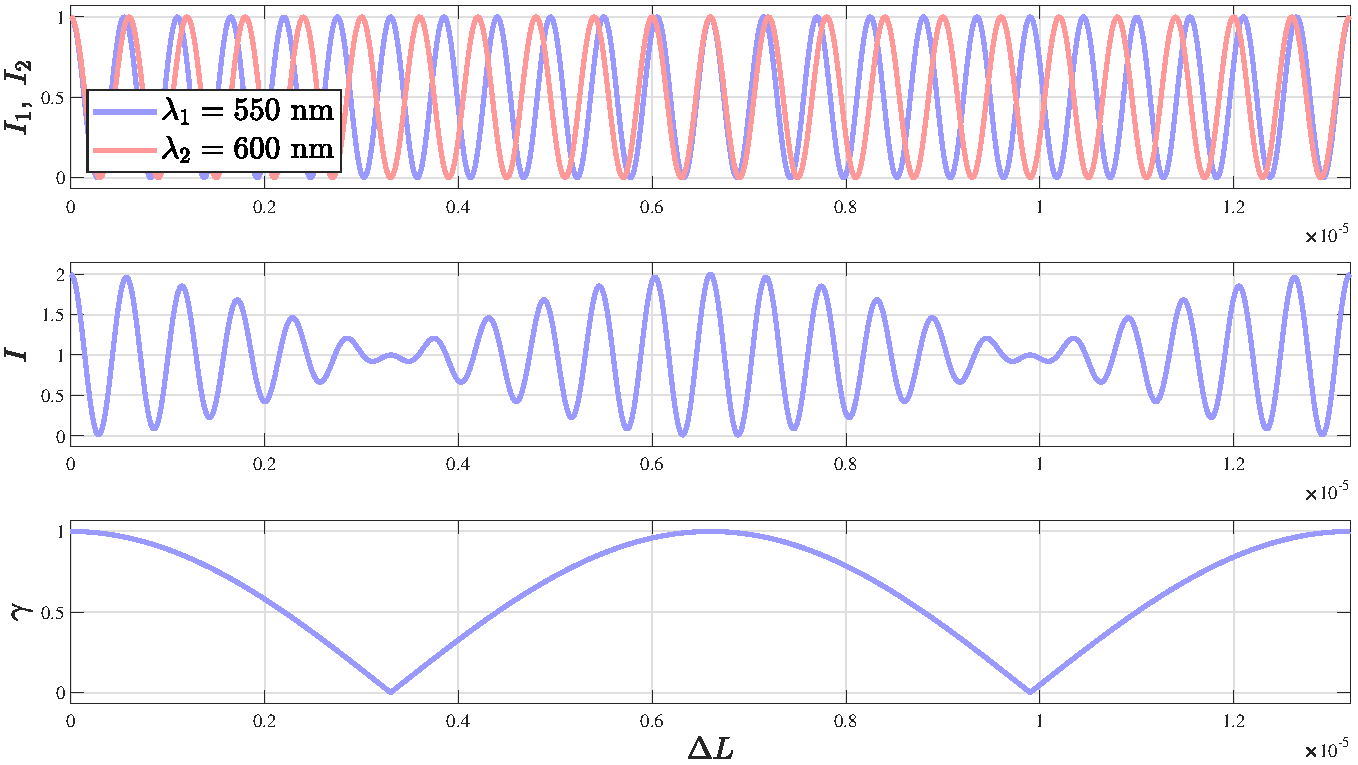
\includegraphics[width=0.85\columnwidth]{assets/3/迈克尔逊干涉_双色光源.pdf}
\caption{ 双色光源的对比度分布情况}\label{双色光源的对比度分布情况}
\end{figure}


设一个周期的条纹数为 $N$($\gamma$ 从 1 到 0 再回到 1),则:
\begin{equation}
N \cdot \lambda = \frac{2 \pi}{\frac{1}{2}\Delta k} = 2 \cdot \left(\frac{1}{2} \frac{\lambda_0^2}{\Delta \lambda}\right) \Longrightarrow N = \frac{\lambda_0}{\Delta \lambda}
\end{equation}


\subsection{(均匀) 连续谱迈克逊干涉}

上面考虑的是线光谱,对于连续光谱,有光谱密度 $i = i(\lambda)$,总光强 $I = \int i(\lambda)\ \mathrm{d}\lambda$。当然,也可以用空间角频率 $k$ 作变量。考虑以 $k_0$ 为中心,宽为 $\Delta k$ 的均匀连续光谱 $i(k)$,我们有:
\begin{gather}\label{光谱宽度对对比度的影响}
i (k) = 
\begin{cases}
    \frac{I_0}{\Delta k}, & |k - k_0| < \frac{\Delta k}{2} \\
    0, & |k - k_0| > \frac{\Delta k}{2}
\end{cases} ,\quad \gamma = \gamma(\Delta L) = \left| \frac{\sin \left(\frac{\Delta k \Delta L}{2}\right)}{\frac{\Delta k \Delta L}{2}} \right| = \left| \sinc \left( \frac{1}{2}\Delta k \Delta L\right) \right| 
\\
I = \int i(k)\left[1 + \cos (k \Delta L)\right] \ \mathrm{d}k = I_0 \left[ 1 + \sinc \left( \frac{1}{2}\Delta k \Delta L\right) \cdot \cos (k_0 \Delta L)\right]
\end{gather}

上面的结果与 \ref{杨氏实验中光源位置和宽度对干涉条纹的影响} 节 “杨氏实验中光源位置和宽度对干涉条纹的影响” 中光源宽度对干涉条纹的影响完全同构,图像也是同构的。我们定义最大光程差 $\Delta L_{\max} = \frac{2 \pi}{\Delta k} \approx \frac{\lambda^2}{\Delta \lambda}$,这是条纹对比度第一次下降到 0 时对应的光程差。

\subsection{马赫-曾德尔干涉}

原理与迈克尔逊干涉仪类似,我们不多赘述。

\section{光场的空间相干性与时间相干性}\label{光场的空间相干性与时间相干性}

\subsection{波列长度、发光线度与光谱宽度}

在杨氏双缝干涉中,我们讨论了光源的线度(宽度)对干涉图样的影响,得到了极限宽度 $b_0 = \frac{\lambda R}{d}$,它是中心条纹对比度第一次为 0 时的光源宽度;在迈克尔逊干涉中,我们又讨论了发光光谱对干涉图样的影响,得到了最大光程差 $\Delta L_{\max} = \frac{2 \pi}{\Delta k} = \approx \frac{\lambda^2}{\Delta \lambda}$,这是条纹对比度第一次下降到 0 时对应的光程差。

上面的例子告诉我们,光源的发光线度与光谱宽度会对干涉性产生影响,前者影响的是 {\color{red} 空间相干性},描述同一时刻不同位置的条纹对比度变化情况,后者影响的是 {\color{red} 时间相干性},描述同一位置不同时刻的条纹对比度变化情况。另外,光源的波列长度也会影响其干涉性(详见 \ref{产生干涉的前提条件} 节“产生干涉的前提条件”)
\\

现实中常可以见到这样的例子:有一些光源,它们具有一定的发光宽度,不能看作理想的点光源。当光源宽度较大时,光源不同部分发出的光的叠加,会导致条纹的对比度降低(甚至为 0),称为空间不相干。

还有一些光源是多频光源(或具有一定光谱宽度,详见表 \ref{光谱宽度对光源单色性的影响})。波长差别极小时(通常是 $10^{-2}$ nm 级),不同波长相互叠加导致条纹对比度降低(但仍可见);波长差别较大时,$\cos(\Delta \alpha)$ 的周期远小于 $\tau$,积分项为零,也只能发生非相干叠加。以两频光源为例,发出时间角频率为 $\omega_1$ 和 $\omega_2$ 的光,则在同一位置,相位差 $\Delta \alpha = (k_2 - k_1)x - (\omega_2 - \omega_1)t$ 是 $t$ 的函数,当曝光时间 $\tau$ 远大于调制周期 $T = \frac{2 \pi}{\omega_1 - \omega_2}$ 时,积分项 $\frac{1}{\tau}\int_{0}^{\tau}  \cos(\Delta \alpha) \mathrm{d} t$ 趋于 0,得到 $I = I_1 + I_2$,也是非相干叠加。

总而言之,影响光源相干性的条件大致有三个方面:波列持续时间 $\tau_0$、光源宽度 $d$ 和发光光谱 $i = i(\lambda)$。现实中的光源总是有一定发光线度、一定光谱宽度、且波列长度有限的,没有任何一种光源在上面三个方面都做到极好。因此,在设计干涉实验时,需要依据光源的特性,选择合适的实验方案,或者依据实验弱化了哪些因素的影响,选择合适的光源。

\begin{table}[H]\centering
    %\renewcommand{\arraystretch}{1.5} % 调整行间距为 1.5 倍
    %\setlength{\tabcolsep}{1.5mm} % 调整列间距
    \caption{\textbf{光谱宽度对光源单色性的影响}}
    \label{光谱宽度对光源单色性的影响}
\begin{tabular}{cccccccccc}\toprule
    光谱宽度 $\Delta \lambda$ & 光源单色性  \\
    \midrule
    10 nm & 极差 \\
    1 nm &  较差 \\
    $10^{-3}$ nm & 较好 \\
    $10^{-6}$ nm & 极好 \\
    \bottomrule
\end{tabular}
\end{table}

\subsection{相干孔径角与空间相干性}

在杨氏双缝干涉中,即相干孔径角 $\Delta \theta_0 \approx \tan \left(\Delta \theta_0\right) = \frac{d}{R}$ 为双孔对光源中心所张角度。记光源面积为 $A_s$,则距离光源 $R$ 处的相干面积 $A_c$: 
\begin{equation}
A_c = \frac{\lambda^2}{A_s} R^2
\end{equation}
相干面积 $A_c$ 与光源面积 $A_s$ 成反比,在相干面积内,取两点作为双孔(次波源),可以得到一定的相干性。这是空间相干性的具体体现之一。

\section{法布里-珀罗干涉仪 (Fabry-Perot Interferometer)}

在 \ref{多光束薄膜干涉} 节“多光束薄膜干涉”中,我们讨论过多光束薄膜干涉的原理,法布里-珀罗干涉仪就是一种利用多光束薄膜干涉的仪器。

\subsection{单色光谱}

法布里-珀罗干涉仪如图 \ref{法布里-珀罗干涉仪} 所示,两片玻璃板中间夹有介质(可以是空气),玻璃片内侧表面镀银以增强反射率。需要注意,应将夹在中间的介质视为薄膜,而不是玻璃板,并且镀银相当于改变了薄膜的反射率。细致的讨论表明,在分析的过程中忽略玻璃板和反射膜带来的额外影响(包括相位差、反射透射率等),仍可得到正确且精度极高的结论\footnote{详见参考文献 \cite{Optics} Page 530}。因此,在后文我们只考虑“空气-薄膜-空气”模型,并视 $R$ 为薄膜表面的反射率。
\begin{figure}[H]\centering
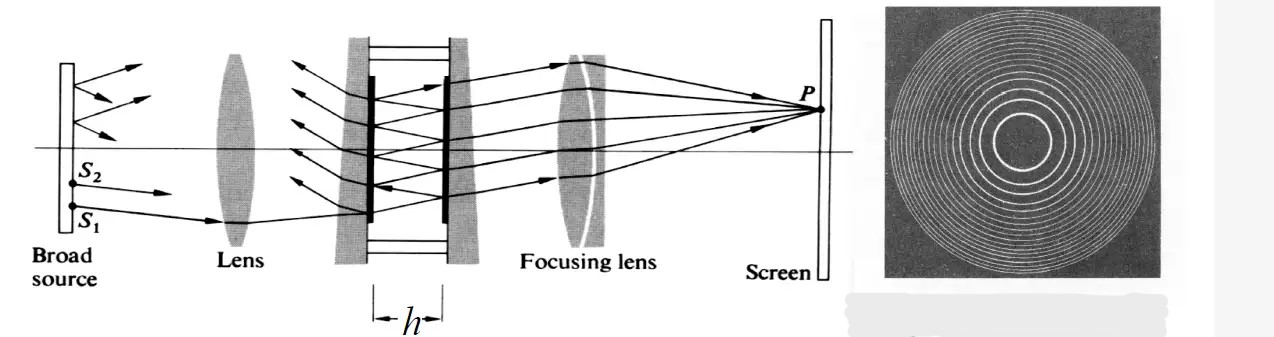
\includegraphics[width=0.9\columnwidth]{assets/3/法布里-珀罗干涉仪.jpg}
\caption{\bfseries 法布里-珀罗干涉仪}\label{法布里-珀罗干涉仪}
\end{figure}
如果以单色扩展光源入射,透射光汇聚到屏幕上,得到等倾干涉条纹(由 $\theta_k$ 提供相位变化)。与迈克尔逊干涉条纹相比,两者都是同心圆,但 F-P 条纹要细锐得多。设薄膜宽度为 $h$,折射率 $n_f$,空气折射率为 1,则薄膜干涉的关键公式如下: 
\begin{gather}
    T_{F-P} = \frac{1}{1 + F \sin^2 \frac{\delta}{2}},\quad R_{F-P} = \frac{F \sin^2 \frac{\delta}{2}}{1 + F \sin^2 \frac{\delta}{2}},  \quad F = \frac{4R}{(1 - R)^2},\quad \delta = \frac{4 \pi n_f d \cos \theta_f}{\lambda_i},\quad m = \frac{\delta}{2}
\end{gather}
在本节后文,我们简记 $\lambda = \lambda_i$ 为光波在空气中的波长,$n_f$ 为玻璃板之间薄膜的折射率,$\theta = \theta_k$ 为薄膜中的折射角(即内角),并称入射角 $\theta_i$ 为外角。则 $\delta$ 可写为 $\delta = \frac{4 \pi n d \cos \theta}{\lambda}$。
\vspace*{-5mm}
\begin{center}\noindent\begin{minipage}{0.48\columnwidth}
    \hspace*{2em} 透射峰的性质可由半峰宽 $\varepsilon$、半峰内角宽度 $\Delta \theta_f$和半峰外角宽度 $\Delta \theta_i$ 来描述。其中,半峰宽指给定 $R$ 时,FP 透射率 $T_{F-P} = T(\delta)$ 图像中 $T_{F-P} = 0.5$ 对应的峰宽,如图 \ref{半峰宽} 所示。而内角宽度是图像 $T_{F-P} = T(\theta_f)$ 的半峰宽、外角宽度是 $T_{F-P} = T(\theta_i)$ 的半峰宽。半峰内角宽度也常简称为角宽度,记为 $\varepsilon_{\theta_f}$\footnote{有的教材中也记作 $\Delta \theta_f$。}。
\begin{gather}
    \varepsilon_{\delta} = 4 \arcsin \left(\frac{1}{\sqrt{F} }\right) 
    \\
    \varepsilon_{\theta_f} = \frac{\lambda}{\pi n d \sin \theta_f\sqrt{F}}
    \\
    \varepsilon_{\theta_i} = \frac{n \lambda}{\pi d\sin \theta_i \sqrt{F}} 
\end{gather}
\end{minipage}\hfill\begin{minipage}{0.48\columnwidth}
    \begin{figure}[H]\centering
        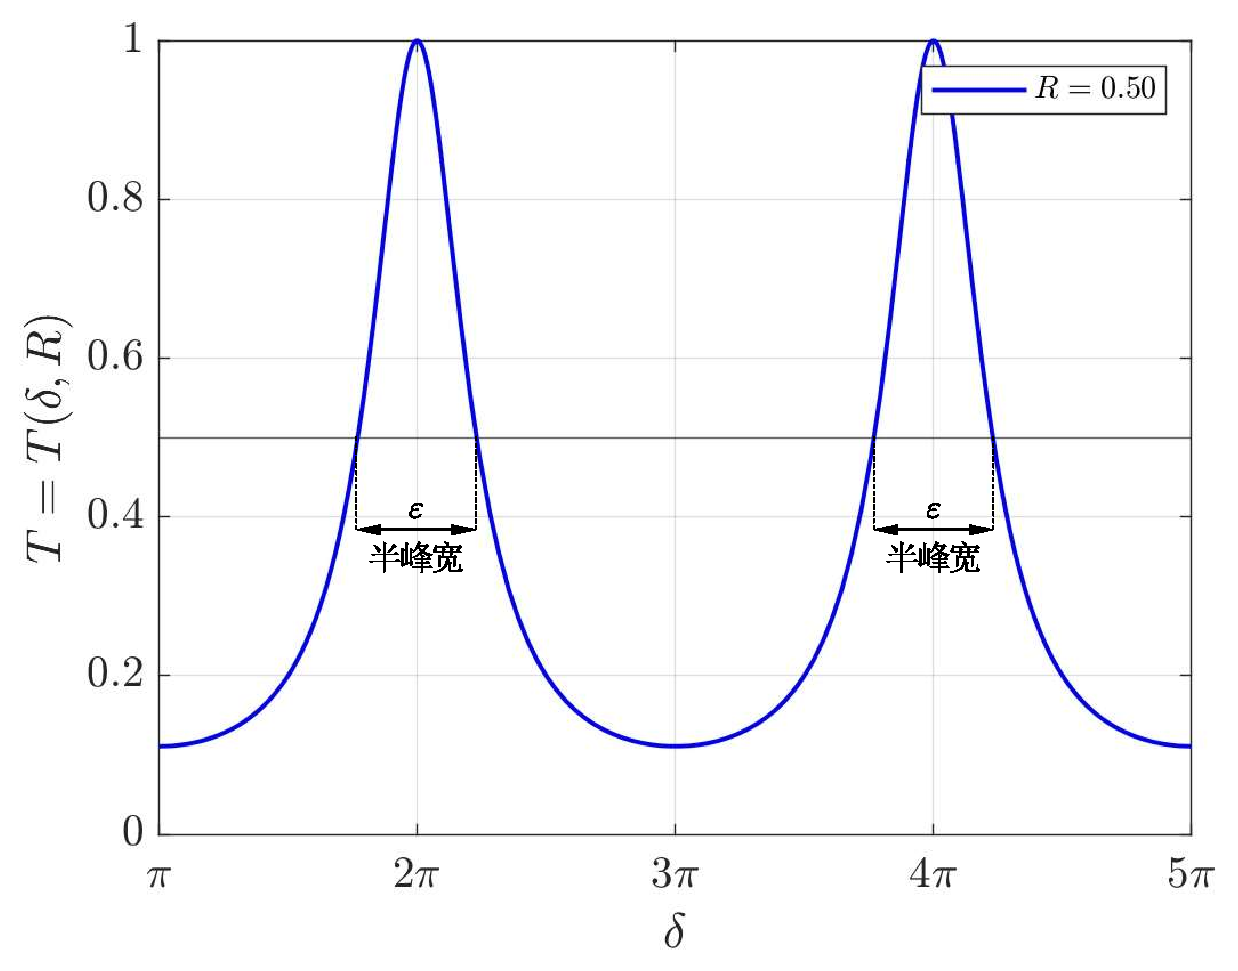
\includegraphics[width=\columnwidth]{assets/3/半峰宽.pdf}
        \caption{\bfseries 半峰宽 $\varepsilon_{\delta}$}\label{半峰宽}
        \end{figure}
\end{minipage}\end{center}

通常情况下,镀膜后的 $R$ 在 $ [0.895, 0.94]$ 内,在此区间内 $F \in [324.7166, 1044.4444]$ 相当大,此时可近似 $\varepsilon_{\delta} \approx\frac{4}{\sqrt{F}}$,所得半峰宽 $\varepsilon_{\delta}$ 的误差不超过 $ 1.1409\times 10^{-4} $。常见的法布里-珀罗干涉仪在可见光波段的锐度 $\mathscr{F}$ 约为 30(对应 $R = 0.9006$),也有特殊的能做到 1000。


所得干涉条纹的明显程度可由透射光对比度 $\gamma_{T_{F-P}}$(简记为 $\gamma$)和锐度 $\mathscr{F}$ 来描述。
\begin{gather}
\gamma = \frac{2R}{1 + R^2}
,\quad 
\mathscr{F} = \frac{2\pi}{\varepsilon_{\delta}} = \frac{\pi}{2 \arcsin \left(\frac{1}{\sqrt{F}}\right)}
\end{gather}

图 \ref{法布里-珀罗干涉仪各参数变化} (a) 展示了对比度 $\gamma$、半峰宽 $\varepsilon_{\delta}$ 和锐度 $\mathscr{F}$ 随反射率 $R$ 的变化情况;图 \ref{法布里-珀罗干涉仪各参数变化} (b)\footnote{图 \ref{法布里-珀罗干涉仪各参数变化} 源码见附录 \ref{法布里-珀罗干涉仪各参数变化 源码}} 展示了透射率 $T = T(\delta, R)$ 的变化情况。

\begin{figure}[H]\centering
\begin{subfigure}[t]{0.49\columnwidth}\centering
    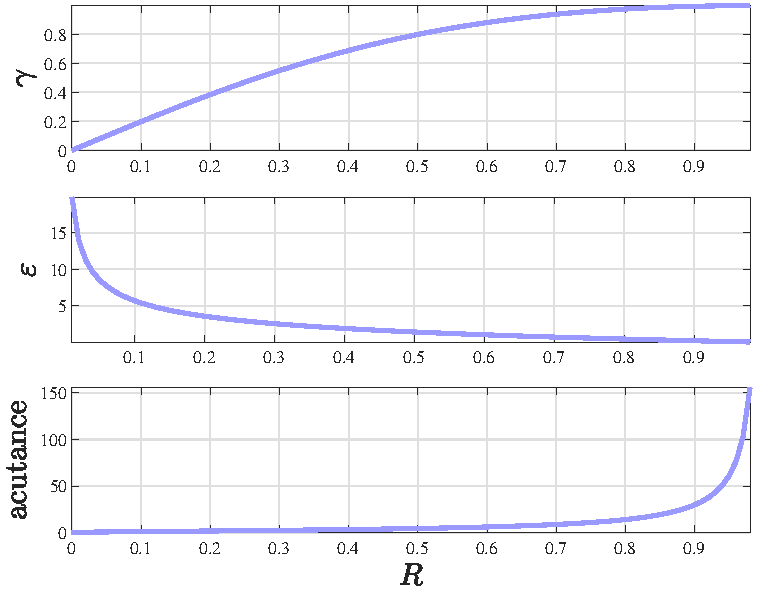
\includegraphics[height=190pt]{assets/3/对比度、半峰宽和锐度随反射率 R 的变化情况.pdf}
    \caption{\bfseries 对比度 $\gamma$、半峰宽 $\varepsilon_{\delta}$ 和锐度 $\mathscr{F}$ 随反射率 $R$ 的变化情况 }
\end{subfigure}\hfill
\begin{subfigure}[t]{0.49\columnwidth}\centering
    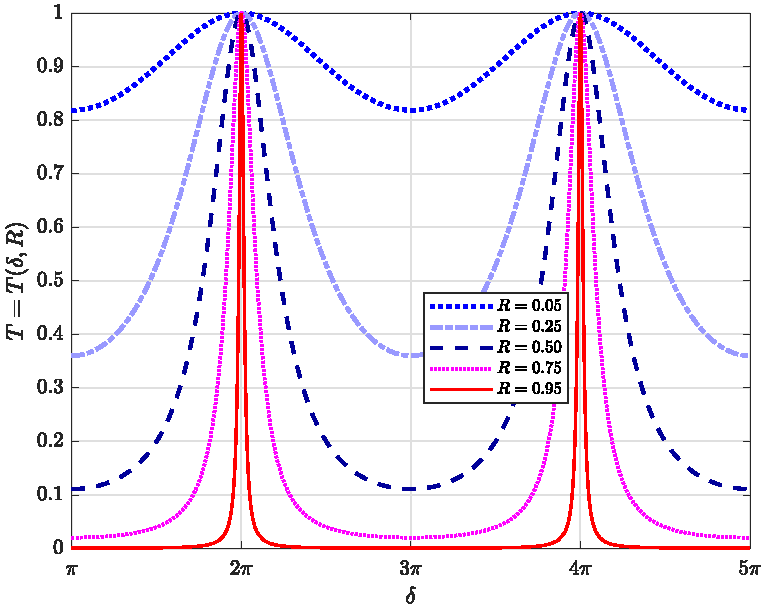
\includegraphics[height=190pt]{assets/3/透射率 T 随 R 和 delta 的变化.pdf}
    \caption{\bfseries 透射率 $T = T(\delta, R)$ 随 $R$ 和 $\delta$ 的变化情况 }
\end{subfigure}
\caption{\bfseries 法布里-珀罗干涉仪各参数变化 }\label{法布里-珀罗干涉仪各参数变化}
\end{figure}


\subsection{双色光谱}

当光源不可视为单色光时,例如两个波长相近的双色光,所形成的等倾干涉条纹(F-P 条纹)就会有稍微不同的半径。这个现象可以用于分辨精细谱线,因此有必要讨论条纹的色分辨能力。

两谱线第 $m$ 级亮纹间的内角距离记作 $\delta \theta_f^m$(注意不是 $\delta \cdot \theta$,而是类似 $\Delta \theta$的记法),或者简记为 $\delta \theta_m$,并简记第 $m$ 级亮纹的内角宽度 $\varepsilon_{\theta_{f, m}}$ 为 $\varepsilon_{\theta_m}$,则有:
\begin{equation}
\delta \theta_m = \frac{{\color{red} m} \Delta \lambda}{2nd\sin \theta_m},\quad \varepsilon_{\theta_m} = \frac{\lambda}{\pi n d \sin \theta_m\sqrt{F}}
\end{equation}

判断能否分辨两谱线,通常采用泰勒判据或瑞丽判据\footnote{此处列出的瑞丽判据是大 $F$ 下的近似判据,详见参考文献 \cite{Optics} Page 532。实际中主要采用泰勒判据。},如下:
\begin{gather}
    \text{Taylor Criterion: \quad } \delta \theta_m \geq \varepsilon_{\theta_m} \Longrightarrow m \geqslant \frac{2\lambda_0}{\pi \sqrt{F} \Delta \lambda}
    \\
    \text{Rayleigh Criterion: \quad } \delta \theta_m \geqslant \frac{4.2}{\sqrt{F}} \Longrightarrow m \geqslant \frac{8.4 n h \sin \theta_m}{\Delta \lambda \sqrt{F} }
\end{gather}

在泰勒判据下,当条纹级数 $m$ 满足判据时,此条纹可以被分辨。需要注意,上面的所称的各级亮纹,其 0 级亮纹不在观察屏中心,而是在无穷远处。这是因为多光束薄膜干涉中,$\delta = \frac{4 \pi n_f d \cos \theta_f}{\lambda_i}$,$\theta_f = 0$ 时,$\delta $ 有最大值,$\theta_f \to \frac{\pi}{2}$ 时,$\delta \to 0$。而习惯上我们称 $\delta = 0$ 的位置为 0 级条纹,因此在这里,0 级条纹无穷远,随着 $m$ 的增大,条纹逐渐向中心靠拢。

并且可以知道,$\theta_f = 0$ 时对应的最高级条纹(位于屏幕最中间的条纹,不一定是中心点)为:
\begin{equation}
m_{\max} =  \left \lfloor \frac{\delta}{2\pi} \right \rfloor_{\theta_f = 0} = \left \lfloor \frac{2nd}{\lambda_0} \right \rfloor,\quad \text{或}\  m_{\max} = \frac{2nd}{\lambda_0}
\end{equation}

依泰勒判据,当所有条纹都可分辨时($\forall\ m \geqslant 1$),得到 $\Delta \lambda \geqslant \frac{2\lambda_0}{1\cdot \pi \sqrt{F}}$,将后者称为可分辨的最小波长差;存在可分辨条纹时($\exists\ m \geqslant 1$),得到 $\Delta \lambda \geqslant \frac{2\lambda_0}{m_{\max}\cdot \pi \sqrt{F}}$,将后者称为极限波长差。
\begin{equation}
    (\Delta \lambda)_{\min} = \frac{1}{{\color{red} 1}}\cdot \frac{2\lambda_0}{\pi \sqrt{F}} = \frac{2\lambda_0}{\pi \sqrt{F}}
    ,\quad 
    (\Delta \lambda)_{\lim} = \frac{1}{{\color{red} m_{\max}}}\cdot \frac{2\lambda_0}{\pi \sqrt{F}} = \frac{\lambda_0^2}{\pi n d \sqrt{F}  }
\end{equation}

$\Delta \lambda$ 越大时,谱线越容易被分辨,但当其大到一定程度时,会发生条纹的越级。由于波长短的条纹更密,所以临界情况是 $ \lambda_0 - \frac{\Delta \lambda}{2}$ 的最高级条纹 ($m_{\max}$) 越过 $ \lambda_0 + \frac{\Delta \lambda}{2}$ 的次级条纹 ($m_{\max} - 1$)。记此时的波长宽为自由光谱范围 (Free Spectral Range),记作 $\left(\Delta \lambda\right)_{\text{fsr}}$。由于中心处 $\theta = 0$,且 $m = \frac{\delta}{2\pi} = \frac{2 nd }{\lambda}$,得到:
\begin{equation}
\begin{cases}
    \lambda + \frac{\Delta \lambda}{2}: & m_{\max} = \frac{2 n d}{\lambda + \left(\Delta \lambda\right)_{\text{fsr}}} 
    \\ 
    \lambda - \frac{\Delta \lambda}{2}: & m_{\max} - 1 = \frac{2 n d}{\lambda - \left(\Delta \lambda\right)_{\text{fsr}}}
\end{cases}\Longrightarrow 
\left(\Delta \lambda\right)_{\text{fsr}} = \frac{\lambda_0}{m_{\max}} = \frac{\lambda_0^2}{2 n d} 
\end{equation}

也就是说,要在不发生条纹越级的条件下分辨谱线,谱宽 $\Delta \lambda$ 需要小于自由光谱宽度 $\left(\Delta \lambda\right)_{\text{fsr}}$。在此前提下,$\Delta \lambda$ 越大,谱线的分辨性越好。


进一步地,对任意一个光谱仪,我们可以定义它的色分辨本领为 $\mathscr{R} = \frac{\lambda_0}{\left(\Delta \lambda\right)_{\lim}}$,色分辨本领越高,表示仪器对谱线的分辨能力越强,分辨率越高。特别地,F-P 干涉仪也可看作是一种光谱仪,有:
\begin{equation}
\mathscr{R} = \frac{\lambda_0}{\left(\Delta \lambda\right)_{\lim}} = \frac{\lambda_0}{\frac{\lambda_0^2}{\pi n d \sqrt{F} }} = m_{\max} \cdot \frac{\pi \sqrt{F} }{2} = \frac{\pi n d \sqrt{F}}{\lambda_0}
\end{equation}



\subsection{连续光谱}

本节仅考虑 $\theta \to 0$ 的情况。当光源具有自由光谱时,F-P 薄膜(也称为 F-P 腔)具有“选频”的效果。具体表现是,光在 F-P 腔内多次相干叠加,使透射光谱结构明显区别于入射光谱,将连续光谱变为离散的准分立谱,也即最终接收到的光谱,如图 \ref{F-P 腔对连续谱的选择作用} 所示。
\begin{figure}[H]\centering
\includegraphics[width=0.8\columnwidth]{assets/3/F-P 腔.jpg}
\caption{\bfseries F-P 腔对连续谱的选择作用}\label{F-P 腔对连续谱的选择作用}
\end{figure}
出现纵模的波长满足 $2nd = m\lambda_m$,因此谱线具有相同的纵模间距(“纵模”即为谱线中的“峰”),且可以计算其半峰频宽:
\begin{equation}
\nu_m = \frac{mc}{2nd},\quad \Delta \nu = \nu_{m+1} - \nu_m = \frac{c}{2nd},\quad \varepsilon_{\nu, m} = \frac{2c}{m \pi \lambda\sqrt{F}} = \frac{c}{\lambda^2} \cdot \frac{\left(\Delta \lambda\right)_{\min}}{m}
\end{equation}
由此可以发现,$\varepsilon_{\nu, m}$ 对应的波长宽度 $\varepsilon_{\lambda, m} = \frac{\lambda^2}{c} \varepsilon_{\nu, m}$ 恰好是 $\frac{\left(\Delta \lambda\right)_{\min}}{m}$。


%巧合的是,$I_T = I_T(\lambda)$ 图像中的半峰宽 $\varepsilon_{\lambda, m} = \frac{2\lambda_0}{\pi m \sqrt{F} } $ 恰好是泰勒判据中的 $\Delta \lambda \geqslant \frac{2\lambda_0}{\pi m \sqrt{F} }$。

\subsection{光学谐振腔}

上面的法布里-珀罗干涉仪,也常称为 F-P 标准具,或简称为标准具。光学谐振腔本质上也是一个 F-P 标准具,只是光学谐振腔的腔体结构更加特殊。通常情况下,谐振腔的两侧是一对的高反射镜(也可以是平面镜、球面镜等),光源在腔体内部,发出的光在腔内来回反射,最终形成透射光谱。
详见 \href{https://www.zhihu.com/question/476559619/answer/3015092750}{知乎:光学微腔和光学谐振腔有什么区别} 以及 \href{https://www.thorlabs.com/newgrouppage9.cfm?objectgroup\_id=9021}{ThorLabs: 法布里-珀罗干涉仪教程}。

\section{激光(略)}

\newpage
\section{章末总结}
本章的内容框架大致为:
\begin{gather*}
\text{第三章:干涉}
\begin{cases}
    \text{分波前}
        \begin{cases}
            \text{杨氏双缝干涉} 
                \begin{cases}
                    \text{理想光源} \\ 
                    \text{有宽度光源}
                \end{cases}
            \\ \text{菲涅尔双面镜} \\ 
            \text{菲涅尔双棱镜} \\ 
            \text{劳埃镜}
        \end{cases} 
    \\\text{分振幅} 
        \begin{cases}
            \text{薄膜干涉 (双光束)} 
                \begin{cases}
                    \text{等厚干涉} 
                        \begin{cases}
                            \text{劈尖干涉}\\
                            \text{牛顿环}
                        \end{cases}
                    \\ \text{等倾干涉} 
                        \begin{cases}
                            \text{等倾干涉仪} \\ 
                            \text{迈克尔逊干涉} 
                                \begin{cases}
                                    \text{单色光谱} \\ 
                                    \text{双色光谱} \\ 
                                    \text{连续光谱}
                                \end{cases}
                            \\\text{马赫曾德尔干涉}
                        \end{cases}
                \end{cases}
            \\ \text{薄膜干涉 (多光束) : }\text{法布里-珀罗干涉}
            \begin{cases}
                \text{单色光谱} \\ 
                \text{双色光谱} \\ 
                \text{连续光谱}
            \end{cases}
        \end{cases}
\end{cases}
\end{gather*}

下面给出相关的公式:
\begin{align*}
&\text{常识}
\begin{cases}
    \text{可见光范围} 
        \begin{cases}
            400 \ \mathrm{nm} \sim 750 \ \mathrm{nm} \\ 
            4.0 \times 10^{14} \ \mathrm{Hz} \sim 7.5 \times 10^{14} \ \mathrm{Hz}
        \end{cases}
    \\\text{典型折射率:} n_{\text{水}} = \frac{4}{3} = 1.33,\ n_{\text{玻璃}} = 1.5
\end{cases}
\\ &
\text{杨氏双缝干涉}
\begin{cases}
    \Delta L = \frac{nd}{D} x = \frac{d}{D} x\ (n=1)  \\ 
    \Delta x = \frac{D}{nd} \lambda = \frac{D}{d} \lambda\ (n=1) \\
    \delta x = - \frac{D}{R} \lambda \\ 
    b_0 = \frac{R}{nd}\lambda = \frac{R}{d}\lambda\ (n=1) \\ 
    bd < \lambda R
\end{cases}
,\ \text{菲涅尔双面/棱镜}
\begin{cases}
    \Delta x = \frac{D}{d}\lambda \\ 
    D = B + C \\ 
    d = \theta B \\ 
    l = \theta C \\ 
    \theta = 
    \begin{cases}
        2\alpha &, \text{双面镜} \\ 
        2(n_L-1)\alpha & , \text{双棱镜}
    \end{cases}
\end{cases}
\\ &
\text{劳埃镜}
\begin{cases}
    d = 2a \\ 
    l \text{\ 用相似三角形计算}
\end{cases}
\end{align*}

\newpage
\begin{align*}
&
\text{光场相干性} 
\begin{cases}
    \text{空间相干性}
        \begin{cases}
            \text{孔径角:} \theta_0 = \frac{\lambda}{b} \\ 
            \text{相干面积:} A = \left(R \theta_0\right)^2 = \frac{R^2\lambda^2}{b^2}
        \end{cases}\\ 
    \text{时间相干性}
        \begin{cases}
            \text{波列宽:} \Delta L < l_0 = c_0\tau_0 \\ 
            \text{光谱宽:} \Delta L < l_0 = \frac{\lambda_0^2}{\Delta \lambda}
        \end{cases}
\end{cases}
\\ &
\text{薄膜干涉 (双光束)}
\begin{cases}
\Delta L = 2n_fd \cos \theta_f + \frac{\lambda}{2} \\ 
\Delta l = 2n_fd \cos \theta_f \\ 
m_{\max} = \frac{2n_fd}{\lambda} \\ 
\text{等厚干涉} 
    \begin{cases}
        \text{劈尖干涉} 
            \begin{cases}
                \Delta d = \frac{\lambda}{2} \\ 
                \Delta x = \frac{\Delta d}{\tan \alpha} \approx \frac{\lambda}{2 \alpha} \\
                \text{暗:}d_m = \frac{\lambda}{2} \cdot m \\ 
                \text{明:}d_m = \frac{\lambda}{2} \cdot \left(m + \frac{1}{2}\right)
            \end{cases}\\ 
        \text{牛顿环}
            \begin{cases}
                \text{暗:} r_m = \sqrt{R\lambda m} \\ 
                \text{明:} r_m = \sqrt{R\lambda \left(m + \frac{1}{2}\right)} \\ 
                \Delta r_m = \sqrt{R\lambda} \left(\sqrt{m + \frac{1}{2}} - \sqrt{m}\right) = \sqrt{R\lambda}\cdot \frac{1}{2\left(\sqrt{m + \frac{1}{2}} + \sqrt{m}\right)}
            \end{cases}
    \end{cases}\\ 
\text{等倾干涉 ($n_f = 1$)}
    \begin{cases}
        \text{等倾干涉仪} 
        \begin{cases}
            \text{亮:}\Delta L = m\lambda \Longrightarrow \cos \theta_m = \frac{\lambda}{2nd}\cdot \left(m - \frac{1}{2}\right) \\ 
            \text{暗:}\Delta L = \left(m + \frac{1}{2}\right)\lambda  \Longrightarrow \cos \theta_m = \frac{\lambda}{2nd}\cdot m \\ 
            r_m = A \cdot \tan \theta_m \approx A \theta_m \\
            \Delta r_m = A \Delta \theta_m = A \cdot \frac{\lambda}{2d \sin \theta_m} = \frac{A\lambda}{2d \theta_k} 
        \end{cases}
        \\ \text{迈克尔逊干涉}
            \begin{cases}
                \text{单色谱}
                    \begin{cases}
                        \text{以中心为零级:} 
                        \begin{cases}
                            2d\left(1 - \cos \theta_m\right) = \lambda m\\ 
                            \theta_m = \sqrt{\frac{m\lambda}{d}}
                        \end{cases}\\ 
                        \text{精密测长:} 2 n \Delta d = N\lambda
                    \end{cases} 
                \\\text{双色谱} 
                    \begin{cases}
                        \gamma = \left| \cos \left(\frac{1}{2}\Delta k \Delta L\right) \right| \\ 
                        \left(\Delta L\right)_{\max} = \frac{1}{2}\cdot \frac{\lambda^2}{\Delta \lambda} \\ 
                        N_{\text{circle}} = \frac{2\left(\Delta L\right)_{\max}}{\lambda} =  \frac{\lambda}{\Delta \lambda}
                    \end{cases}
                \\\text{连续谱} 
                    \begin{cases}
                        \gamma = \left| \sinc \left(\frac{1}{2}\Delta k \Delta L\right) \right| \\ 
                        \left(\Delta L\right)_{\max} = \frac{\lambda^2}{\Delta \lambda} \\ 
                        N_{\text{circle}} = \frac{2\left(\Delta L\right)_{\max}}{\lambda} =  \frac{2\lambda}{\Delta \lambda}
                    \end{cases}
            \end{cases}
    \end{cases}
\end{cases}
\end{align*}

\begin{align*}
    \text{薄膜干涉 (多光束) : }
    \begin{cases}
        \Delta l = 2n_fd \cos \theta_f \\
        \delta = \frac{2\pi}{\lambda} \cdot \Delta l = \frac{4 \pi n_f d \cos \theta_f}{\lambda} \\
        F = \frac{4R}{(1 - R)^2} \\
        T_{\text{F-P}} = \frac{1}{1 + F \sin^2 \frac{\delta}{2}},\ R_{\text{F-P}} = 1 - T_{\text{F-P}} = \frac{F \sin^2 \frac{\delta}{2}}{1 + F \sin^2 \frac{\delta}{2}}\\
        \text{法布里-珀罗干涉}
            \begin{cases}
                \text{单色谱}
                    \begin{cases}
                        \text{半峰宽:}\varepsilon_{\delta} = 4 \arcsin \left(\frac{1}{\sqrt{F} }\right) \\
                        \text{内角宽:} \varepsilon_{\theta_f} = \frac{1}{n \sin \theta_f} \cdot \frac{\lambda}{\pi d \sqrt{F}} = \frac{1}{\sin \theta_i} \cdot \frac{\lambda}{\pi d \sqrt{F}} \\
                        \text{外角宽:} \varepsilon_{\theta_i} = \frac{n}{\sin \theta_i} \cdot \frac{n \lambda}{\pi d \sqrt{F}} \\
                        \text{对比度:} \gamma = \frac{2R}{1 + R^2} \\
                        \text{锐度:} \mathscr{F} = \frac{2\pi}{\varepsilon_{\delta}} \\
                    \end{cases} \\ 
                \text{双色谱}
                    \begin{cases}
                        \text{内角距离:} \delta \theta_m = \frac{1}{n \sin \theta_{f,m}} \cdot m \cdot \frac{\Delta \lambda}{2d} \\ 
                        \text{Talor 判据:} \delta \theta_m \geq \varepsilon_{\theta_m} \Longrightarrow m \geq \frac{2\lambda_0}{\pi \sqrt{F} \Delta \lambda} = \frac{1}{\frac{\pi \sqrt{F}}{2}}\cdot \frac{\lambda}{\Delta \lambda_0}\\
                        \text{最小分辨率:}\left(\Delta \lambda\right)_{\min} = \frac{2\lambda_0}{\pi \sqrt{F}} \\ 
                        \text{极限分辨率:}\left(\Delta \lambda\right)_{\lim} = \frac{\left(\Delta \lambda\right)_{\min}}{m_{\max}} = \frac{\lambda_0^2}{\pi n d \sqrt{F}} \\ 
                        \text{自由光谱宽度:}\left(\Delta \lambda\right)_{\text{fsr}} =\frac{\lambda_0^2}{2nd} \\ 
                        \text{色分辨本领:}\mathscr{R} = \frac{\lambda_0}{\left(\Delta \lambda\right)_{\lim}} = \frac{m_{\max}\pi \sqrt{F}}{2} = \frac{\pi n d \sqrt{F}}{\lambda_0}
                    \end{cases}
                \\\text{连续谱}
                \begin{cases}
                    \text{纵模波长:} m\lambda = 2nd \Longrightarrow \lambda = \frac{2nd}{m} \\ 
                    \text{纵模频率:}\nu_m = \frac{c}{\lambda_m} = \frac{mc}{2nd} \\ 
                    \text{纵模间距:}\Delta \nu = \frac{c}{2nd} \\ 
                    \text{半峰频宽:}\varepsilon_{\nu, m} = \frac{c}{\lambda^2}\left(\Delta \lambda\right)_{\min} \cdot \frac{1}{m}  = \frac{2c}{m \pi \lambda \sqrt{F}}
                \end{cases}
            \end{cases}
    \end{cases}
\end{align*}

\chapter{光的衍射}\thispagestyle{fancy}

什么是衍射?衍射是波动现象的一个普遍特征,每逢波阵面(不论是声波、物质波还是光波)的一部分以某种方式受到阻碍时就会发生,如果在遇到障碍物(不论是透明的还是不透明的)的进程中,波阵面上一个区域的振幅或相位受到改变,波就会偏离直线传播的方向,这种现象叫做“衍射”。

越过障碍物的波阵面的各区段因干涉而引起特定的能量密度分布,叫做“衍射图样”。干涉和衍射之间并不存在实质性的物理差别。然而习惯上(虽然并不总是恰当),当考虑的只是几个波源的叠加时说是干涉,而讨论大量波源(可以是无限个)的叠加则说是衍射。尽管如此,同一现象在有些地方叫做多光束干涉,而在另一地方则叫做光栅衍射。

\section{衍射发生的条件}

\subsection{惠更斯-菲涅尔原理}

惠更斯原理揭示了波在空间中传播时的姿态(即波阵面的形状和传播反向等),但它与波长无关,这无法解释为什么声波容易绕过障碍物而激光却不易。惠更斯-菲涅尔原理可以解释这一现象:

\begin{LineTheorem}[惠更斯-菲涅尔原理]\label{惠更斯-菲涅尔原理}
在给定时刻,波阵面上每一未被阻挡的点起着次级球面子波(频率与初波相同)波源的作用。对障碍物外任一点,各子波在这一点的振幅和相位通常不同,此点的振幅(电磁波即电场)是所有这些子波的相干叠加。
\end{LineTheorem}

从之前的方法来看,我们可以将障碍物或小孔看作是有宽度的光源,或 $N$ 个全同的波源($N$ 趋于无穷),它们的行为将在后文进行讨论。定性地说,当障碍物的线度在几个波长的尺度时,衍射现象将十分明显。障碍物线度再变小,例如 0.1 个波长,电磁场的边界效应将成为主要部分,这不在本课讨论的范围内。

应当指出,求一个特定衍射问题的严格解是光学中最难处理的问题之一,这涉及到许多更为复杂的理论。就目前的学习而言,惠更斯-菲涅尔原理是简单且足够精确的。

\subsection{菲涅尔衍射与夫琅禾费衍射}

对其上有一小孔的不透明屏幕,小孔附近的衍射现象(近场)与远场截然不同(尽管后者是前者的一个特例)。我们将小孔附近的衍射现象称为菲涅尔衍射(近场衍射),将离小孔足够远处衍射现象称为夫琅禾费衍射(远场衍射)。

孔径的线度是是否发生夫琅禾费衍射的决定性判据。作为一条经验定则,设孔径(或障碍物)的最大宽度为 $b$,小孔到光源 $S$ 和观察点 $P$ 的距离分别为 $d_S$、$d_P$,则发生夫琅禾费衍射的充分条件是:
\begin{equation}
    d_S > \frac{b^2}{\lambda} ,\quad d_P > \frac{b^2}{\lambda}
\end{equation}
当满足判据,发生夫琅禾费衍射时,可以认为所有的子波源在 $P$ 点振幅都相同,而菲涅尔衍射通常不能作这样的近似。

如图 \ref{近场和远场的不同衍射现象} 所示,左半边从下至上逐渐从近场过渡到远场,右半边显示了衍射角 $\theta_0$ 与小孔宽度 $b$ 的关系:
\begin{equation}
\theta_0 = \frac{\lambda}{b}
\end{equation}
小孔宽度 $b$ 越小,衍射角越大,所有子波叠加之后越接近球面波。由于远场衍射更为简单,后文我们会先讨论远场,再讨论近场。

\begin{figure}[H]\centering
    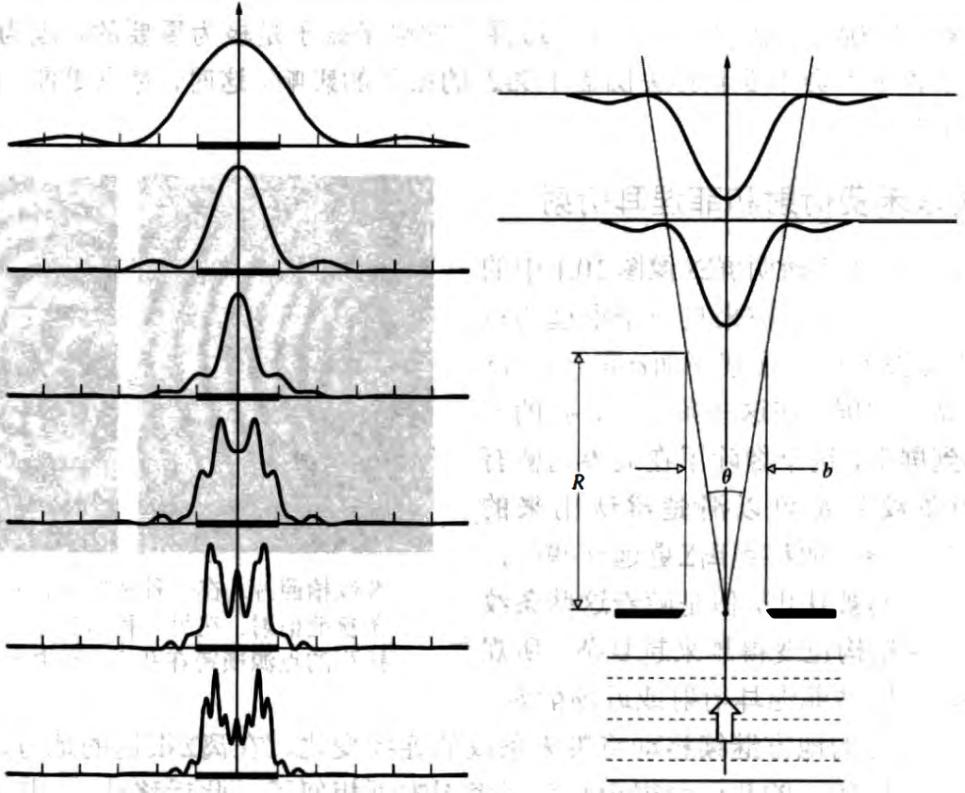
\includegraphics[width = 0.6\columnwidth]{assets/4/4.1 衍射发生的条件.jpg}
    \caption{近场和远场的不同衍射现象}\label{近场和远场的不同衍射现象}
\end{figure}

\section{全同振子阵列与理想线光源}

\subsection{全同振子阵列}
如图 \ref{单缝衍射的理想模型} (a),考虑 $N$ 个相干的点源振子构成的直线阵列,各个振子在一切方面(包括偏振方向)都完全相同,并且认为振子间没有固定的相位差。

\begin{figure}[H]\centering
\begin{subfigure}[b]{0.5\columnwidth}\centering
    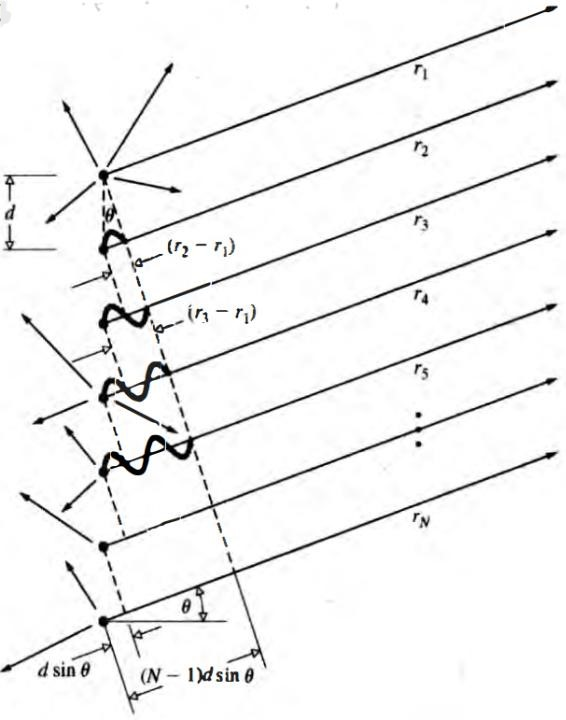
\includegraphics[height=180pt]{assets/4/4.2 全同振子阵列.jpg}
    \caption{全同振子阵列}
\end{subfigure}\hfill
\begin{subfigure}[b]{0.5\columnwidth}\centering
    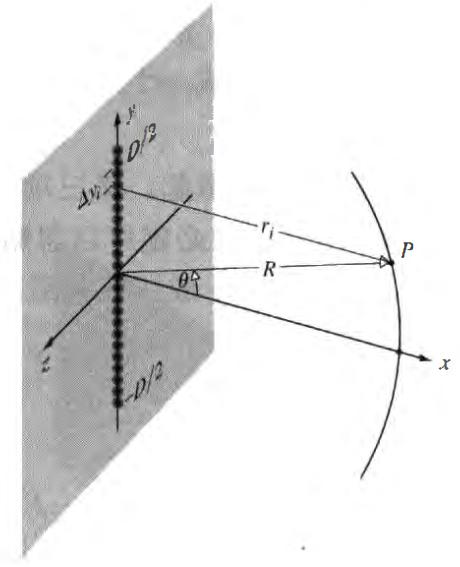
\includegraphics[height=180pt]{assets/4/4.2 理想相干线光源.jpg}
    \caption{理想相干线光源}
\end{subfigure}
\caption{单缝衍射的理想模型}
\label{单缝衍射的理想模型}
\end{figure}

对远场中的一点 $P$,可以认为各子波在此点有相同的振幅,即 $E_0(r) = E_0(r_1) = \cdots = E_0(r_N)$,总电场强度是 $N$ 个振子的场强叠加:
\begin{equation}
E = \sum_{m=1}^{N}E_0(r) e^{i\left(kr_m - \omega t\right)} = E_0(r) e^{-i\omega t} e^{ikr_1} \sum_{m=1}^{N}e^{ik(r_m - r_1)}
\end{equation}
记相邻点远之间的相差为 $\delta$,则 $\delta = kd\sin \theta \Longrightarrow k(r_m - r_1) = (m-1)\delta$,于是:
\begin{align}
    E 
    &= E_0(r) e^{-i\omega t} e^{ikr_1} \sum_{m=1}^{N}e^{i(m-1)\delta} 
    = E_0(r) e^{-i\omega t} e^{ikr_1} \frac{e^{iN\delta} - 1}{e^{i\delta} - 1} \\ 
    &= E_0(r) e^{-i\omega t} e^{ikr_1} e^{i\left(\frac{(N-1)}{2}\delta\right)} \left(\frac{\sin \frac{N\delta}{2}}{\sin \frac{\delta}{2}}\right) 
    = E_0(r) e^{i\left(kr_1 + \frac{N - 1}{2}\delta - \omega t\right)} \left(\frac{\sin \frac{N\delta}{2}}{\sin \frac{\delta}{2}}\right) \\
    & = E_0(r)\left(\frac{\sin \frac{N\delta}{2}}{\sin \frac{\delta}{2}}\right)\cdot e^{i\left(kR - \omega t\right)}
\end{align}
其中 $R = \frac{1}{2}(N - 1)d\sin \theta + r_1$ 是阵列中心到 $P$ 点的距离。于是可以得到辐照度(通量密度)的分布:
\begin{equation}
I = I_0 \frac{\sin^2 \left(N\frac{\delta}{2}\right)}{\sin^2 \left(\frac{\delta}{2}\right)} = I_0\frac{\sin^2 \left(N \frac{kd}{2}\sin \theta \right)}{\sin^2 \left( \frac{kd}{2}\sin \theta \right)},\quad \sin \theta \approx \frac{y}{R}
\end{equation}
其中 $I_0$ 是任意一个波源在距离为 $r$ 时的辐照度。$N = 0$ 时 $I = 0$,$N = 1$ 时 $I = I_0$,$N = 2$ 时 $I = 4I_0\cos^2 \frac{\delta}{2} = 2I_0\left(1 + \cos \delta\right)$,这些与之前的内容都是相符的。

由表达式可以知道,$I_0$ 的主极大出现在 $\frac{\delta}{2} = m \pi ,\ m = 0, \pm 1, ...$ 的方向上,也即 $d \sin \theta_m = m \lambda$。并且相邻两个主极大之间有 $(N-2)$ 个副极大,即相邻两个主峰之间有 $(N-2)$ 个辅峰。

令 $\lambda = 1 \ \mathrm{m}$,$d = 5 \ \mathrm{m}$,作出 $I_0$ 随 $\sin \theta$ 的变化情况,如图 \ref{全同振子阵列的辐照度分布} 所示。可以看到,随着 $N$ 的增大,辐照度的最大值 $I_{\max} = N^2 I_0$ 越大.

\begin{figure}[H]\centering
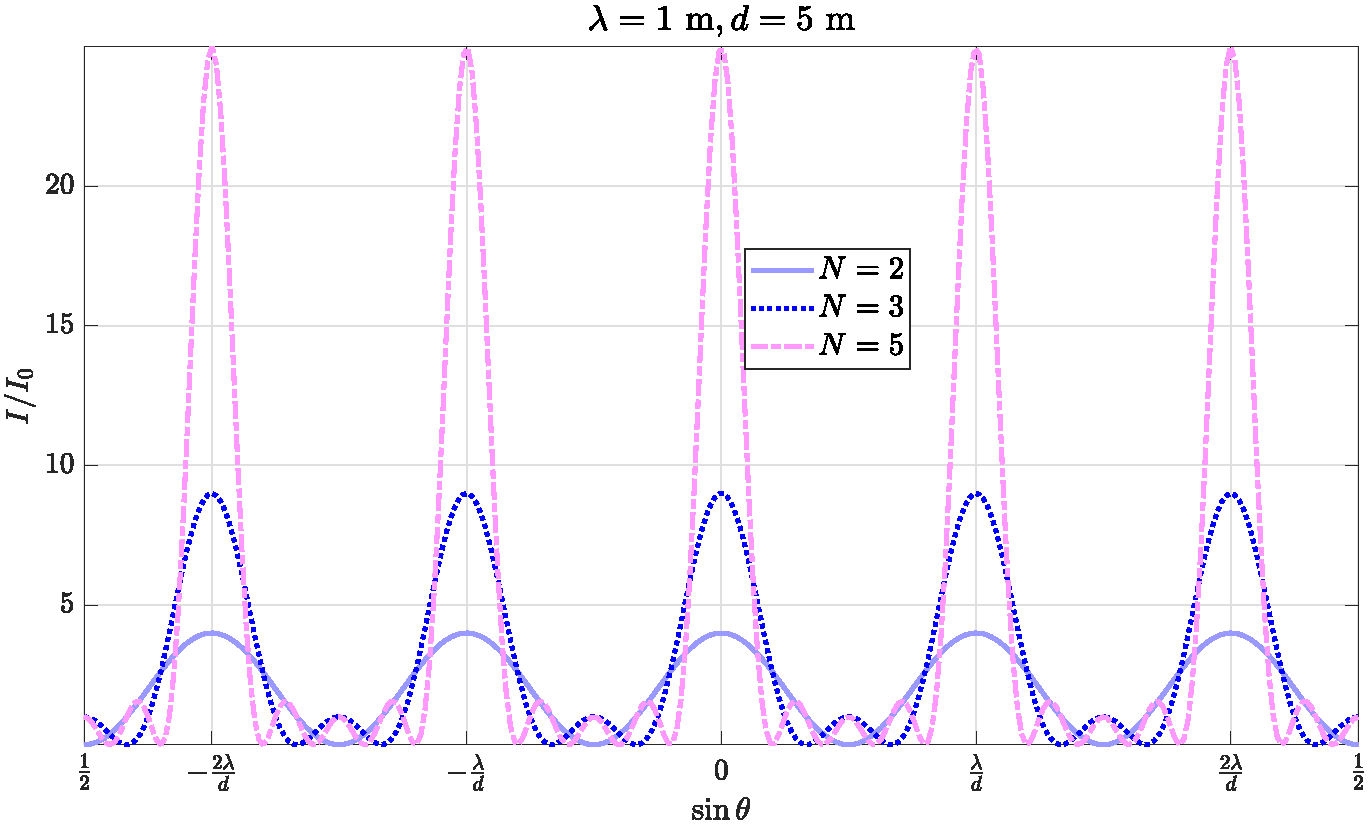
\includegraphics[width=0.95\columnwidth]{assets/4/4.2 全同振子.pdf}
\caption{全同振子阵列的辐照度分布}\label{全同振子阵列的辐照度分布}
\end{figure}

\subsection{理想线光源}

如图 \ref{单缝衍射的理想模型} (b),考虑一个宽度为 $D$ 的理想线光源(例如平面波照射宽度远小于 $\lambda$ 的长狭缝),它可以视为无限个全同振子,每一点发射一个球面子波,子波方程为:
\begin{equation}
E_{\text{sub}} = \frac{\varepsilon_0}{r}e^{i(kr - \omega t)}
\end{equation}
其中 $\varepsilon_0$ 称为波源强度(也称光源强度,注意不是真空介电常量)。取阵列上的一段微元 $\ \mathrm{d}y$,其上包含 $\frac{\mathrm{d}y}{D}N$ 个波源(稍后我们会令 $N \to \infty$),则这一段微元对 $P$ 点电场的贡献为:
\begin{equation}
\mathrm{d}E = \frac{N\mathrm{d}y}{D}\cdot \frac{\varepsilon_0}{r}e^{i(kr - \omega t)} = \frac{N\varepsilon_0}{Dr}e^{i(kr - \omega t)} \mathrm{d}y = \frac{\varepsilon_L}{r}e^{i(kr - \omega t)} \mathrm{d}y,\quad \varepsilon_L = \lim_{N\to \infty} \frac{N\varepsilon_0}{D}
\end{equation}
其中 $\varepsilon_L$ 称为单位长度上的波源强度。作积分即得:
\begin{equation}\label{理想线光源积分公式}
E = \varepsilon_L \int_{-\frac{D}{2}}^{+\frac{D}{2}} \frac{e^{i(kr - \omega t)}}{r} \mathrm{d}y,\quad r = r(y)
\end{equation}
对不同位置的点 $P$,上式的近似方式也不同,从而得到不同的结果。相干的线光源现在还不存在物理实体,但它可以为我们提供数学上的启发。

\section{夫琅禾费衍射}

\subsection{单缝远场衍射}

设相比于光源宽度 $D$,观察点 $P$ 离线光源很远,即 $R \gg D$,有近似 $r = R - y\sin \theta$,代入公式 (\ref{理想线光源积分公式}) 进行积分,得到:
\begin{gather}
E = \frac{\varepsilon_L D}{R}\cdot \sinc \left(\frac{1}{2}kD \sin \theta\right) e^{i\left(kR - \omega t\right)}
= \frac{\varepsilon_L D \sinc \beta}{R}  e^{i\left(kR - \omega t\right)},\quad \beta = \frac{1}{2}kD \sin \theta = \frac{\pi D}{\lambda} \sin \theta\\ 
I = I(\theta)= \langle E^2  \rangle_T = \frac{1}{2}\left(\frac{\varepsilon_LD}{R}\right)^2 \sinc^2 \beta,\quad I = I(0) \sinc^2 \beta
\end{gather}
因为 $\beta = \frac{1}{2}kD \sin \theta = \frac{\pi D}{\lambda} \sin \theta $,当 $D \gg \lambda$ 时,随着 $\theta$ 的增大,$\beta$ 急剧增大,$\sinc^2 \beta$ 迅速趋近于 0,。反之,如果 $D \ll \lambda$,$\beta$ 对一切 $\theta \in [0, \frac{\pi}{2})$ 都可近似为 0,此时 $I \equiv I(0)$ 不变(由能量守恒,此值也会趋近于 0),线源就化为一个发射球面波的点源。

在处理单缝衍射时,设缝宽较小而缝长较大,呈竖直方向。那么狭缝的“每一横”(横向的微元)都可视作一个理想线光源,线光源宽度 $D$ 即为狭缝的宽度 $b$。基于此,仍可得到与上面一致的结果。特别地,单缝衍射辐照度的极值发生在:
\begin{gather}
\text{极小值 (为 0) : \ } \beta = m \pi,\ m = \pm 1, \pm 2, ... \Longrightarrow b \sin \theta = m \lambda,\ m = \pm 1, \pm 2, ... \\ 
\text{极大值:} \tan \beta = \beta \Longrightarrow \beta \approx 1.43 \pi, 2.46 \pi, 3.47 \pi, ...
\end{gather}
下表列出了部分极值的角度和相对辐照度大小,以供形成直观的认识。
\vspace*{-5mm}\begin{center}
\noindent\begin{minipage}{0.49\columnwidth}
    \begin{table}[H]\centering
        %\renewcommand{\arraystretch}{1.5} % 调整行间距为 1.5 倍
        %\setlength{\tabcolsep}{1.5mm} % 调整列间距
        \caption{单缝夫琅禾费衍射的极大值}
        \label{单缝夫琅禾费衍射的极大值}
    \begin{tabular}{cccccccccc}\toprule
        $\beta$ (rad) & 归一化振幅 $E_{0, r}$ & 归一化照度 $I_r$ \\
        \midrule
        0            & 1      & 1      \\
        1.4303 $\pi$ & -0.217 & 0.047  \\
        2.4590 $\pi$ & 0.128  & 0.016  \\
        3.4707 $\pi$ & 0.091  & 0.008  \\
        \bottomrule
    \end{tabular}
    \end{table}
\end{minipage}\hfill\begin{minipage}{0.49\columnwidth}
    \begin{table}[H]\centering
        %\renewcommand{\arraystretch}{1.5} % 调整行间距为 1.5 倍
        %\setlength{\tabcolsep}{1.5mm} % 调整列间距
        \caption{单缝夫琅禾费衍射的极小值}
        \label{单缝夫琅禾费衍射的极小值}
    \begin{tabular}{cccccccccc}\toprule
        $\beta$ (rad) & 归一化振幅 $E_{0, r}$ & 归一化照度 $I_r$ \\
        \midrule
        $\pi$  & 0 & 0 \\
        $2\pi$ & 0 & 0 \\
        $3\pi$ & 0 & 0 \\
        $4\pi$ & 0 & 0 \\
        \bottomrule
    \end{tabular}
    \end{table}
\end{minipage}\end{center}


对实验装置而言,如果我们使用能以单缝为轴自由旋转的辐照度计(始终指向狭缝中心),便可以方便的改变角度 $\theta$,此时应选择使 $N = \frac{b}{\lambda}$ 较小的狭缝宽度($b$ 通常在几个波长),以使得主要的图像较好地分布在给定的 $\theta$ 范围内,例如 $[-50^\circ,\ 50^\circ]$。作为一个例子,我们固定 $\lambda = 3 \ \mathrm{cm}$ 不变,作出辐照度 $I$ 随 $\theta \in [-45^\circ,\ 45^\circ]$ 的分布情况,如图 \ref{单缝夫琅禾费衍射} (a) 所示。同时还可讨论中央极大的全峰角宽度 $\xi_{\theta}$ : 
\begin{gather}
I = I(0) \sinc^2 \beta =  I(0) \sinc^2\left( \frac{\pi b}{\lambda} \sin \theta \right) = I(0) \sinc^2\left( N \pi \sin \theta \right) \\ 
b \sin \theta_0 = \lambda \Longrightarrow \xi_{\theta} = 2 \theta_0 = 2 \arcsin \left(\frac{\lambda}{b}\right) = 2 \arcsin \left(\frac{1}{N}\right)
\end{gather}
从公式和图 \ref{单缝夫琅禾费衍射} (a)中可以看到,$N$ 越大,角宽度就越小,若固定 $\lambda$ 不懂,缝宽 $b$ 减小则会使照度的幅度减小。


\begin{figure}[H]\centering
\begin{subfigure}[b]{0.5\columnwidth}\centering
    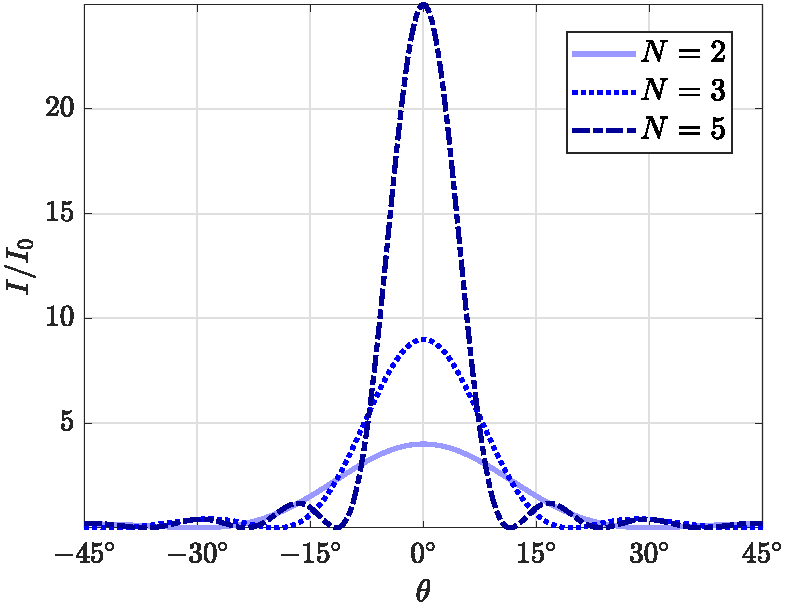
\includegraphics[height=185pt]{assets/4/4.3 辐照度随角度变化.pdf}
    \caption{辐照度随角度 $\theta$ 的变化}
\end{subfigure}\hfill
\begin{subfigure}[b]{0.5\columnwidth}\centering
    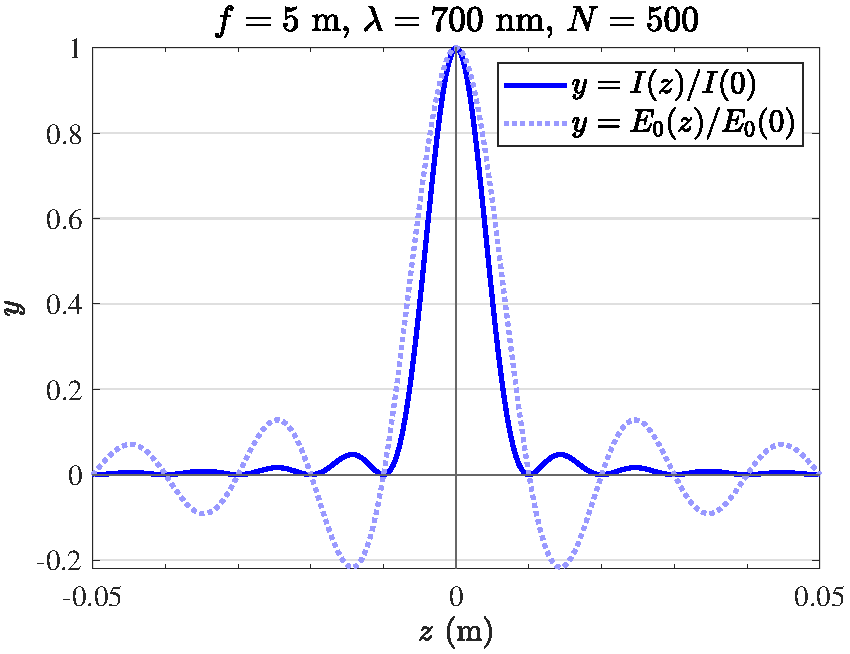
\includegraphics[height=185pt]{assets/4/4.3 辐照度随位置变化.pdf}
    \caption{辐照度随位置 $z$ 的变化}
\end{subfigure}
\caption{单缝夫琅禾费衍射}
\label{单缝夫琅禾费衍射}
\end{figure}

如果采用固定在中轴线上的观察板,由于实际的距离 $R$ 不可能无穷大,因此可以采用图 \ref{用屏幕观察单缝衍射的实验装置} 中的装置。其中,单缝与观察屏之间的透镜 $L_2$ 应紧挨单缝,其线度和焦距都要远大于单缝宽度 $b$,并且观察屏恰好放在 $L_2$ 的焦距处。另外,为了使主要图像集中在观潮屏对应的极小角度范围内,$N$ 应该较大(对可见光而言,通常是几百个波长)。这样,既实现了 $R \to \infty$,又能在接受屏上有较好的衍射现象。

\begin{figure}[H]\centering
\begin{subfigure}[b]{0.57\columnwidth}\centering
    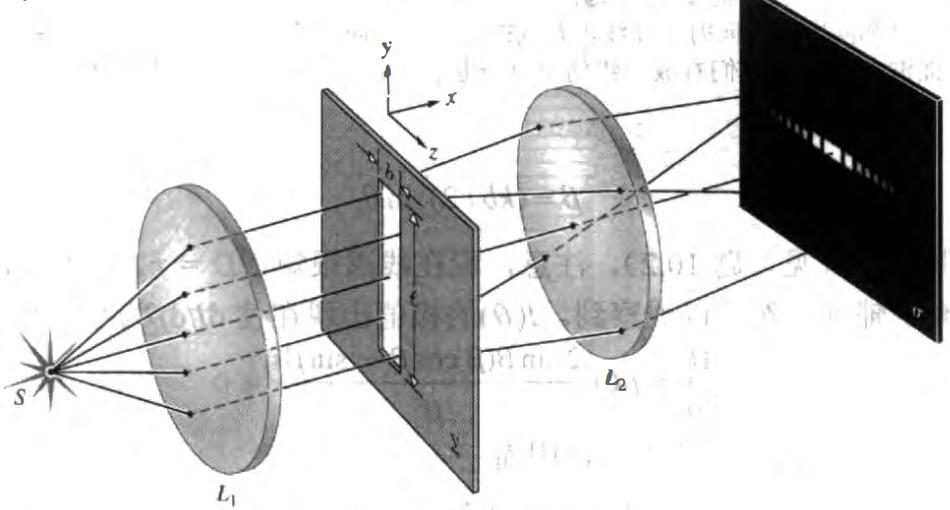
\includegraphics[height=145pt]{assets/4/4.3 辐照度位置仪2.jpg}
    \caption{三维图}
\end{subfigure}\hfill
\begin{subfigure}[b]{0.36\columnwidth}\centering
    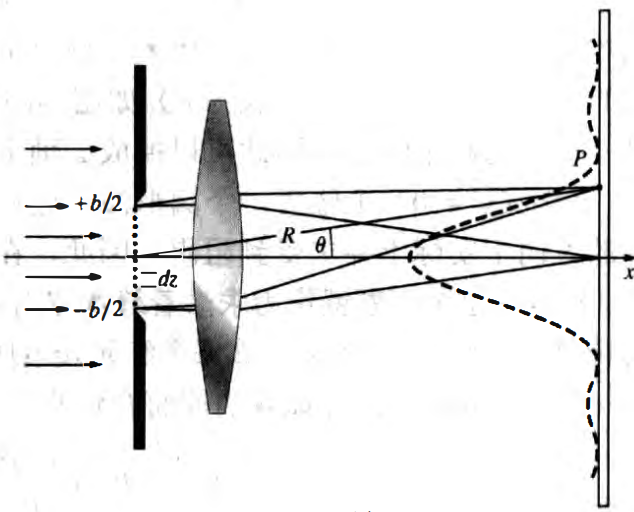
\includegraphics[height=145pt]{assets/4/4.3 辐照度位置仪.png}
    \caption{横剖面}
\end{subfigure}
\caption{用屏幕观察单缝衍射的实验装置}
\label{用屏幕观察单缝衍射的实验装置}
\end{figure}

借助狭缝中心点在屏幕上的成像,可以帮助我们推导辐照度随位置 $z$ 的分布。依据图 \ref{用屏幕观察单缝衍射的实验装置},可以计算 $I = I(z)$ 的表示式,以及中央极大的全峰线宽度 $\xi_z$ : 
\begin{gather}
    \sin \theta \approx \tan \theta = \frac{z}{f} \Longrightarrow I = I(z) = I(0) \sinc^2 \left( \frac{N \pi}{f} z\right) \\ 
    \sin \theta_0 = \frac{\lambda}{b} \Longrightarrow \xi_z = 2 f \tan \theta_0 = 2f\frac{\sin \theta}{\sqrt{1 - \sin^2 \theta}} = \frac{2f}{\sqrt{N^2 - 1}}
\end{gather}


不妨作出 $z \in [-5 \ \mathrm{cm}, 5 \ \mathrm{cm}]$ 时,电场的幅度 $E_0$ 和辐照度 $I$ 的变化情况,如图 \ref{单缝夫琅禾费衍射} (b) 所示。


\subsection{双缝远场衍射}

假设现在有两个宽为 $b$ 的长狭缝,从中心到中心的距离为 $a$,这构成一个由单缝衍射调制过的快速变化的双缝干涉系统,所得到的辐照度分布是双缝衍射后的相干叠加。

如图在远场近似下,积分公式 (\ref{理想线光源积分公式}) 变为:
\begin{gather}
E  = E(z)= \varepsilon_L \left[\int_{-\frac{b}{2}}^{\frac{b}{2}} F(z) \ \mathrm{d}z + \int_{a-\frac{b}{2}}^{a+\frac{b}{2}} F(z) \ \mathrm{d}z\right]
,\quad F(z) = \sin \left(kR - \omega t + kz \sin \theta\right) \\ 
\Longrightarrow E = b\,\varepsilon_L \sinc \beta \left[\sin (kR - \omega t) + \sin (kR - \omega t + 2\alpha)\right] = b\,\varepsilon_L \sinc \beta \cos \alpha \cdot e^{i(kR - \omega t + \alpha)} \\ 
\Longrightarrow I = 4 I_0 \sinc^2 \beta \cos^2 \alpha,\quad \alpha = \frac{1}{2}k a \sin \theta = \frac{\pi a}{\lambda} \sin \theta,\ \beta = \frac{\pi b}{\lambda} \sin \theta
\end{gather}
其中 $I_0$ 是只有单条狭缝时的最大辐照度,系数 4 是因为电场变为两倍时,辐照度变为 4 倍。

在上式中,若 $b$ 非常小($kb \to 0$),则化为理想杨氏实验的表达式;若 $a = 0$,则化为单缝衍射的表达式。记 $m = \frac{a}{b}$,即 $a = mb$,则衍射主峰中可以观察到 $2m-1$ 个极大亮纹,也即除中央亮纹外,两边还各有 $m-1$ 条亮纹。最边缘的两个亮纹事实上被“分割”过,我们没有将其算在辅峰中,称为缺级,如果算入,则应有 $2m + 1$ 个极大峰。



固定 $b = 0.35 \ \mathrm{mm}$ 不变,考虑不同 $m$ 下的衍射图样 ($a = mb$),如图 \ref{双缝衍射图样} 和图 \ref{主峰内双缝衍射图样变化} 所示。

\begin{figure}[H]\centering
    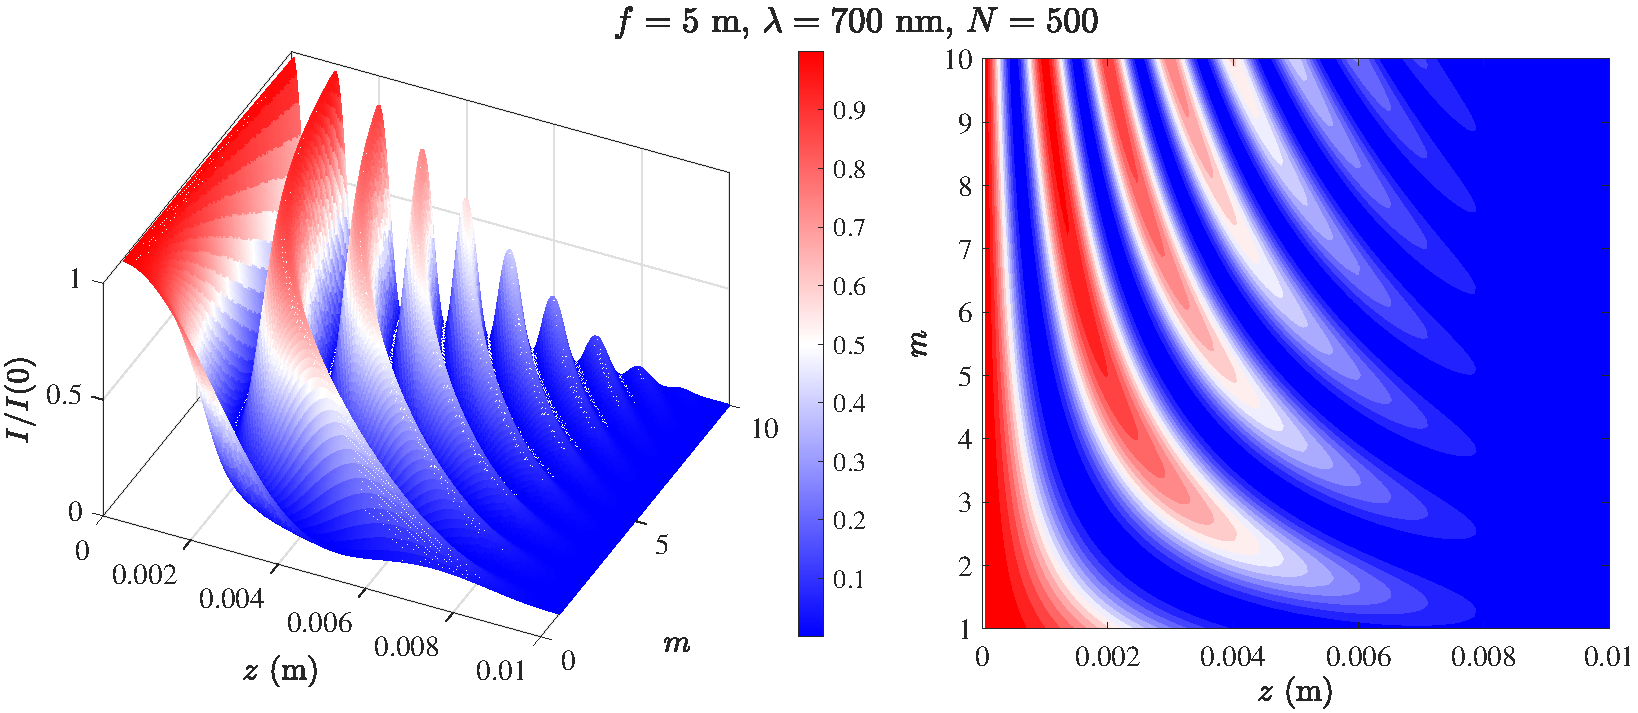
\includegraphics[width=\columnwidth]{assets/4/4.3 m 变化.pdf}
    \caption{单缝主峰内双缝衍射图样随 $m$ 的变化情况}\label{主峰内双缝衍射图样变化}
\end{figure}
\begin{figure}[H]\centering
\begin{subfigure}[b]{0.33\columnwidth}\centering
    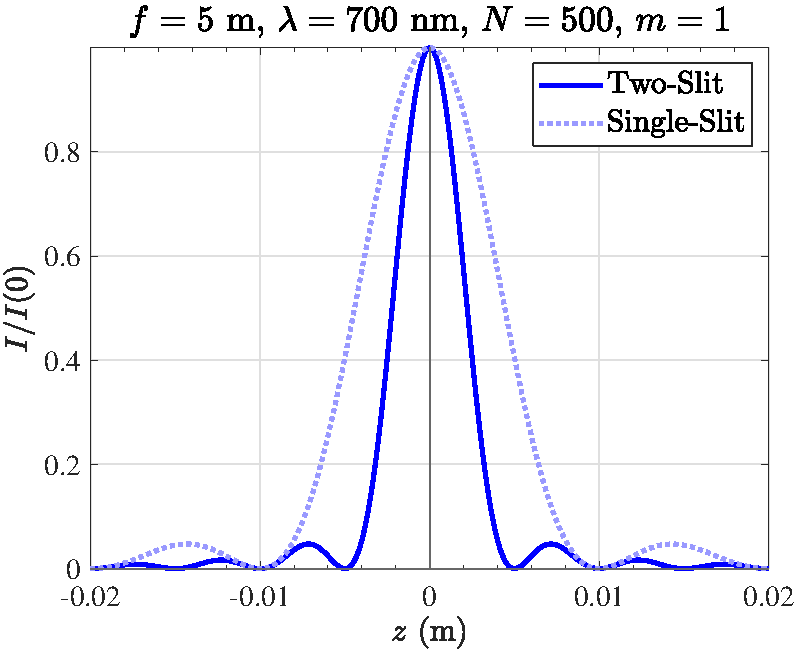
\includegraphics[height=130pt]{assets/4/4.3 m=1.pdf}
    \caption{$m=1$}
\end{subfigure}\hfill
\begin{subfigure}[b]{0.33\columnwidth}\centering
    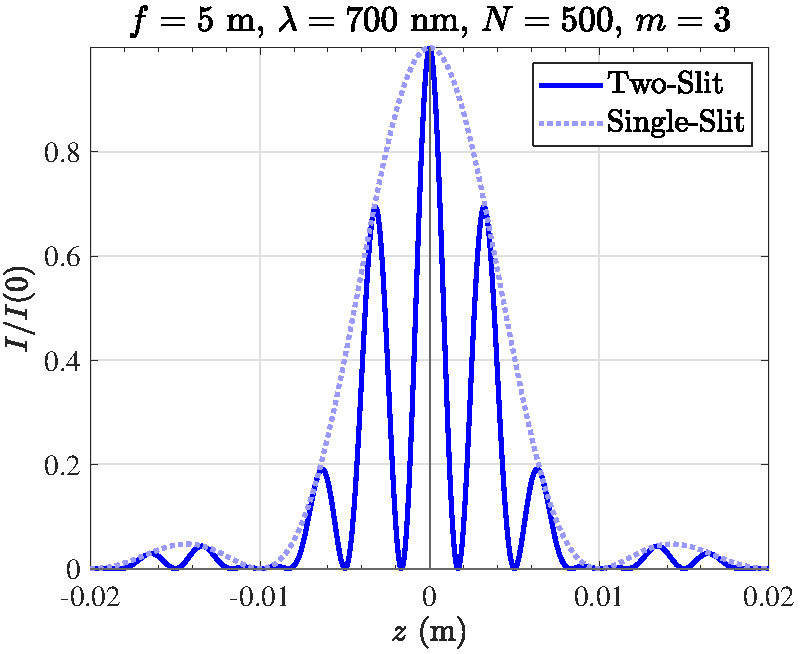
\includegraphics[height=130pt]{assets/4/4.3 m=3.pdf}
    \caption{$m=3$}
\end{subfigure}
\begin{subfigure}[b]{0.33\columnwidth}\centering
    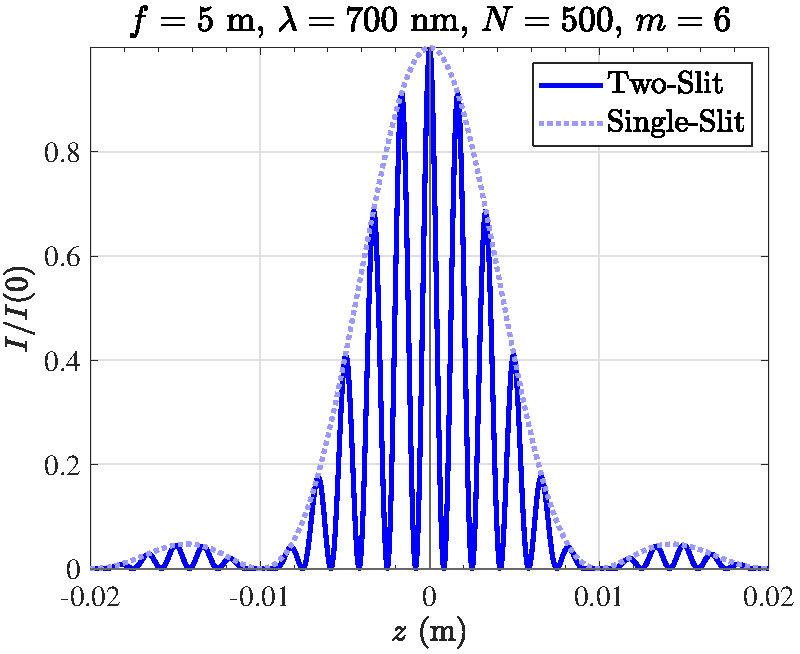
\includegraphics[height=130pt]{assets/4/4.3 m=6.pdf}
    \caption{$m=6$}
\end{subfigure}
\caption{不同 $m$ 下的双缝衍射图样}
\label{双缝衍射图样}
\end{figure}


\subsection{多缝远场衍射}

现在设狭缝的数目为 $N_{\text{slit}} \ (N_{\text{slit}} \geqslant 2)$,或简记为 $N_s$,且相邻狭缝之间的中心距离都为 $a$,则积分式变为:
\begin{gather}
E = \varepsilon_L \sum_{j=0}^{N_s-1} \int_{(j-1)a-\frac{b}{2}}^{(j-1)a\frac{b}{2}} F(z) \ \mathrm{d}z = b \,\varepsilon_L  \sinc \beta \sum_{j=0}^{N_s-1}\sin (kR - \omega t + 2\alpha \cdot j) \\ 
= b \,\varepsilon_L  \sinc \beta e^{i(kR - \omega t)}  \Im \left[ \sum_{j=0}^{N_s-1} \left(e^{i2\alpha}\right)^j \right]
=  b \,\varepsilon_L  \sinc \beta \left(\frac{\sin N_s \alpha}{\sin \alpha}\right) \cdot e^{i\left(kR - \omega t + (N-1)\alpha\right)} \\ 
\Longrightarrow I = I_0 \left( \sinc \beta\right)^2 \left(\frac{\sin N_s \alpha}{\sin \alpha}\right)^2
,\quad \alpha = \frac{1}{2}k a \sin \theta = \frac{\pi a}{\lambda} \sin \theta,\ \beta = \frac{\pi b}{\lambda} \sin \theta
\end{gather}
其中 $I_0$ 是仅有单缝时的辐照度,注意 $I(0) = N_s^2I_0$。主极大峰发生在 $\alpha = m\pi, m = 0, \pm 1, \pm 2, ...$ 的位置(角度)上,这等价于 $a \sin \theta_m = m \lambda$,此时 $\frac{\sin N_s \alpha}{\sin \alpha} = N_s$。相邻两个主峰之间有 $(N_s - 2)$ 个副峰。
\begin{figure}[H]\centering
\begin{subfigure}[b]{0.33\columnwidth}\centering
    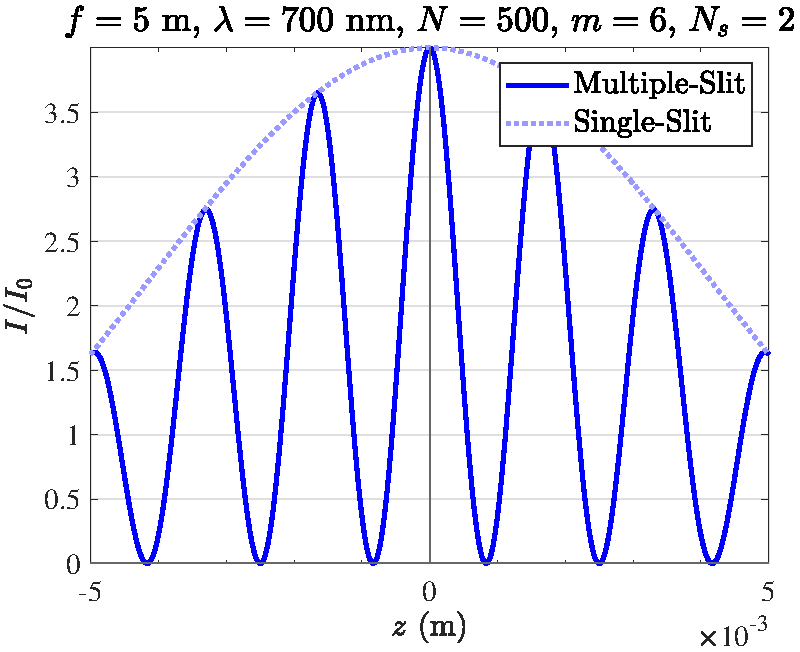
\includegraphics[height=130pt]{assets/4/4.3 N_s=2.pdf}
    \caption{$N_s=2$}
\end{subfigure}\hfill
\begin{subfigure}[b]{0.33\columnwidth}\centering
    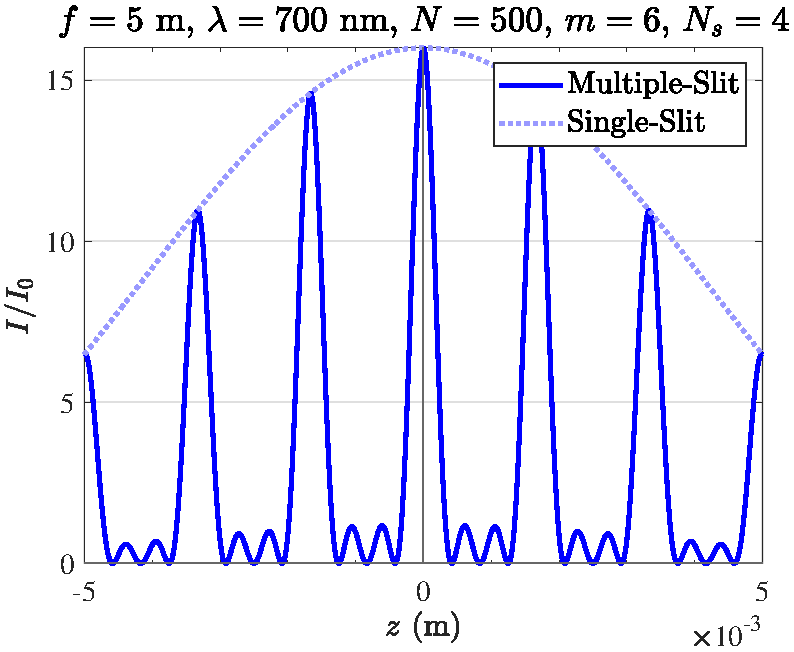
\includegraphics[height=130pt]{assets/4/4.3 N_s=4.pdf}
    \caption{$N_s=4$}
\end{subfigure}
\begin{subfigure}[b]{0.33\columnwidth}\centering
    \includegraphics[height=130pt]{assets/4/4.3 N_s=6.pdf}
    \caption{$N_s=6$}
\end{subfigure}
\caption{不同 $N_s$ 下的多缝衍射图样}
\label{多缝衍射图样}
\end{figure}

从单缝到双缝,是加入了单缝衍射调制后的峰(可以认为是主峰),从双缝再到多峰,便是在这些主峰之间又加入了 $(N_s - 2)$ 个辅峰,并且辅峰得到的能量很少。

\subsection{小孔远场衍射}

在研究具体的矩形孔、圆孔之前,我们先给出小孔衍射的理论基础。仍在夫琅禾费衍射情形下作推导,如图 \ref{任意小孔的夫琅禾费衍射} 所示。
将小孔视为无限个具有面积 $\mathrm{d}A$ 的点光源(发出球面波),我们有:
\begin{gather}
\ \mathrm{d}E = \frac{\varepsilon_A}{r} \cdot e^{i(kr - \omega t)} \ \mathrm{d}A,\quad R  =\sqrt{X^2 + Y^2 + Z^2} \\ 
r  = R\cdot \sqrt{ 1 - \frac{2\left(yY + zZ\right)}{R^2} +  \frac{y^2 + z^2}{R^2} }  \approx  R\left(1 - \frac{\left(yY + zZ\right)}{R^2}  \right) = R - \frac{yY + zZ}{R}
\end{gather}
于是到达 $P$ 点的电场叠加为:
\begin{equation}\label{小孔衍射积分公式}
E = \frac{\varepsilon_A e^{i(kR - \omega t)}}{R} \iint_{A} e^{ik \left(\frac{yY + zZ}{R}\right)} \ \mathrm{d}A
\end{equation}
这便是小孔远场衍射的积分公式。此式没有通解,对于不同类型的小孔,我们可以取不同的近似方法,进而得到具体的结果。
\begin{figure}[H]\centering
    \includegraphics[width=0.5\columnwidth]{assets/4/4.3 小孔衍射.png}
    \caption{任意小孔的夫琅禾费衍射}\label{任意小孔的夫琅禾费衍射}
\end{figure}

\subsection{矩形孔远场衍射}

当小孔是横宽 $a$,纵高为 $b$ 的矩形孔时,如图 \ref{小孔衍射的具体例子} (a)。
\begin{figure}[H]\centering
    \begin{subfigure}[b]{0.5\columnwidth}\centering
        \includegraphics[height=140pt]{assets/4/4.3 矩形孔.png}
        \caption{矩形孔}
    \end{subfigure}\hfill
    \begin{subfigure}[b]{0.5\columnwidth}\centering
        \includegraphics[height=140pt]{assets/4/4.3 圆孔.png}
        \caption{圆孔}
    \end{subfigure}
    \caption{小孔衍射的具体例子}
    \label{小孔衍射的具体例子}
\end{figure}
则积分式 (\ref{小孔衍射积分公式}) 变为:
\begin{gather}
    E = \frac{\varepsilon_{A} e^{i(kR - \omega t)}}{R} \int_{-\frac{b}{2}}^{\frac{b}{2}} e^{ik \cdot \frac{yY}{R}}\ \mathrm{d}y \cdot \int_{-\frac{a}{2}}^{\frac{a}{2}} e^{ik \cdot \frac{zZ}{R}}\ \mathrm{d} \Longrightarrow \\ 
    E = \frac{A\varepsilon_A}{R} \sinc \alpha' \sinc \beta' \cdot e^{i(kR - \omega t)}
    \\ 
    I = I(0)\sinc^2 \alpha \sinc^2 \beta,\quad I(0) = \frac{A^2\varepsilon_A^2}{R^2} 
    \\ 
    \alpha = \frac{1}{2}ka \sin \theta_a = \frac{1}{2}ka\cdot \frac{Z}{R},\quad \beta = \frac{1}{2}kb \sin \theta_b = \frac{1}{2}kb\cdot \frac{Y}{R}
\end{gather}
沿 $a$ 轴方向($\alpha$ 方向)时 $\beta = 0$,辐照度的包络线为 $I = \frac{I(0)}{\alpha^2}$;类似地,沿 $b$ 轴方向($\beta$ 方向)的包络线为 $I = \frac{I(0)}{\beta^2}$。下面的几张图展示了矩形孔的辐照度分布情况。

\begin{figure}[H]\centering
\begin{subfigure}[b]{0.5\columnwidth}\centering
    \includegraphics[height=190pt]{assets/4/4.3 矩形孔辐照度分布 1.pdf}
    \caption{在观察屏上的辐照度分布}
\end{subfigure}\hfill
\begin{subfigure}[b]{0.5\columnwidth}\centering
    \includegraphics[height=190pt]{assets/4/4.3 矩形孔衍射辐照度分布.pdf}
    \caption{沿 $alpha$ 轴的辐照度分布}
\end{subfigure}
\caption{矩形孔的辐照度分布}
\end{figure}

\begin{figure}[H]\centering
    \includegraphics[width=\columnwidth]{assets/4/4.3 矩形孔辐照度分布 3.pdf}
    \caption{辐照度分布细节放大}
\end{figure}

\begin{figure}[H]\centering
\begin{subfigure}[b]{0.56\columnwidth}\centering
    \includegraphics[height=123pt]{assets/4/4.3 矩形孔辐照度分布 4.png}
    \caption{夫琅禾费衍射图}
\end{subfigure}\hfill
\begin{subfigure}[b]{0.44\columnwidth}\centering
    \includegraphics[height=123pt]{assets/4/4.3 矩形孔辐照度分布 5.png}
    \caption{归一化夫琅禾费衍射图样}
\end{subfigure}
\caption{垂直矩形孔(竖直狭缝)的辐照度图像}
\end{figure}


\subsection{圆孔远场衍射}
如图 \ref{小孔衍射的具体例子} (b),对圆孔的情形,我们采用球坐标,则积分式 (\ref{小孔衍射积分公式}) 化为:
\begin{equation}
E = \frac{\varepsilon_A e^{i(kR - \omega t)}}{R} \int_{\rho = 0}^{\rho = a} \int_{\phi = 0}^{\phi = 2\pi} e^{i\left(\frac{k\rho q}{R} \cos (\phi - \Phi)\right)} \,\rho \ \mathrm{\rho} \ \mathrm{\phi}
\end{equation}
由旋转对称性,结果必然与 $\Phi$ 无关,因此不妨令 $\Phi = 0$。为求(表示)此积分结果,我们需要引入(第一类)贝塞尔函数 $J$,类似伽马函数和贝塔函数,它也是由积分定义的,在物理中很常见。定义 0 阶和 $n$ 阶贝塞尔函数如下:
\begin{equation}
J_0(x) = \frac{1}{2\pi} \int_{0}^{2\pi} e^{i x \cos \phi} \ \mathrm{d}\phi
,\quad 
J_n(x) = \frac{i^{-n}}{2\pi} \int_{0}^{2\pi} e^{i(n\phi + x\cos \phi)} \ \mathrm{d}\phi,\quad n = 0, 1, 2, ...
\end{equation}
变量 $x$ 可以是复数。它的一个重要性质是递推关系:
\begin{equation}
    J_0(x) = J_1'(x) + \frac{J_1(x)}{x},\quad \left[x^nJ_n(x)\right]' = x^nJ_{n-1}(x),\quad n = 1, 2, ...
\end{equation}
为了方便后文表示,与依据 $\sin$ 定义 $\sinc$ 时类似,我们也定义 $\Jc$ 函数如下:
\begin{equation}
\Jc_0(x) = \frac{{\color{red} 2} J_0(x)}{x},\quad \Jc_n(x) = \frac{{\color{red} 2} J_n(x)}{x},\quad n = 0, 1, 2, ...
\end{equation} 
分子上的 2 是为了使 $\Jc_1$ 在原点的极限值为 1(类似 $\sinc$ 的极限值)。$J_n(x)$ 和 $\Jc_n(x)$ 在正实轴上的图像如图 \ref{贝塞尔函数及其引申函数} 所示,偶数阶(包括 0 阶)时为偶函数,奇数阶时为奇函数。
\begin{figure}[H]\centering
\begin{subfigure}[b]{0.5\columnwidth}\centering
    \includegraphics[height=180pt]{assets/4/4.3 贝塞尔函数 J.pdf}
    \caption{(第一类) 贝塞尔函数}
\end{subfigure}\hfill
\begin{subfigure}[b]{0.5\columnwidth}\centering
    \includegraphics[height=180pt]{assets/4/4.3 Jc 函数.pdf}
    \caption{定义的 $\Jc$ 函数}
\end{subfigure}
\caption{贝塞尔函数及其引申函数}
\label{贝塞尔函数及其引申函数}
\end{figure}

继续我们的积分,并简记 $\delta = ka \cdot \frac{r}{R} \approx ka \sin \theta $,可以得到:
\begin{gather}
E = \frac{A\varepsilon_A}{R} \Jc_1(\delta) \cdot e^{i(kR - \omega t)} \\ 
I = I(0) \Jc_1^2(\delta),\quad I(0) = \frac{A^2\varepsilon_A^2}{R^2},\quad 
\delta =  ka \cdot \frac{r}{R} \approx ka \sin \theta 
\end{gather}
\vspace*{-6mm}
\begin{figure}[H]\centering
    \includegraphics[width=0.9\columnwidth]{assets/4/4.3 小孔辐照度分布 1.pdf}
    \vspace*{-5mm}
    \caption{在观察屏上的辐照度分布}
\end{figure}
\begin{figure}[H]\centering
    \includegraphics[width=0.93\columnwidth]{assets/4/4.3 小孔辐照度分布 2.pdf}\vspace*{-5mm}
    \caption{辐照度分布细节放大}
\end{figure}
\begin{figure}[H]\centering
\begin{subfigure}[b]{0.5\columnwidth}\centering
    \includegraphics[height=170pt]{assets/4/4.3 圆孔衍射示意图.png}
    \caption{圆孔夫琅禾费衍射的爱里图样}
\end{subfigure}\hfill
\begin{subfigure}[b]{0.5\columnwidth}\centering
    \includegraphics[height=170pt]{assets/4/4.3 圆孔辐照度 3.pdf}
    \caption{辐照度随自变量 $\delta$ 的变化}
\end{subfigure}\vspace*{-3mm}
\caption{圆孔夫琅禾费衍射}
\end{figure}
辐照度的极小值等价于 $J_1(x)$ 的零点(0 除外),极大值等价于 $J_2(x)$ 的零点,为方便参考,我们列出前几个极值的及相对大小:
\begin{center}
\noindent\begin{minipage}{0.49\columnwidth}
    \begin{table}[H]\centering
        %\renewcommand{\arraystretch}{1.5} % 调整行间距为 1.5 倍
        %\setlength{\tabcolsep}{1.5mm} % 调整列间距
        \caption{圆孔夫琅禾费衍射的极大值}
        \label{圆孔夫琅禾费衍射的极大值}
    \begin{tabular}{cccccccccc}\toprule
        $\delta = kar/R$ & 0 & 5.1356 & 8.4172 & 11.6198 \\
        \midrule
        $I/I(0)$ & 1 & 0.0175 & 0.0042 & 0.0016  \\
        \bottomrule
    \end{tabular}
    \end{table}
\end{minipage}\hfill\begin{minipage}{0.49\columnwidth}
    \begin{table}[H]\centering
        %\renewcommand{\arraystretch}{1.5} % 调整行间距为 1.5 倍
        %\setlength{\tabcolsep}{1.5mm} % 调整列间距
        \caption{圆孔夫琅禾费衍射的极小值}
        \label{圆孔夫琅禾费衍射的极小值}
    \begin{tabular}{cccccccccc}\toprule
        $\delta = kar/R$ & 3.8317 & 7.0156 & 10.1735 & 13.3237  \\
        \midrule
        $I/I(0)$ & 0 & 0 & 0 & 0 \\
        \bottomrule
    \end{tabular}
    \end{table}
\end{minipage}\end{center}
为了描述衍射现象的尺度,我们定义辐照度的全峰角宽度 $\xi_{\theta}$,由于辐照度的第一个极小值(零点)在 $\delta = 3.8317$ 处,因此有:
\begin{equation}
ka \sin \theta_0 = 3.8317 \Longrightarrow \xi_\theta = 2 \theta_0 = 2\arcsin \left( \frac{3.8317}{2\pi} \cdot \frac{\lambda}{2a} \right) \approx  \frac{1.22}{\,a\,}\,\lambda = \frac{2.44}{D}\lambda
\end{equation}
常说的“角宽度”便是指 $\xi_\theta$。与单缝衍射时类似,我们使用透镜聚焦出射光,在焦平面上得到衍射图样,此时有全峰(线)宽度 $\xi_z = 2 f\tan \left(\frac{\xi_\theta}{2}\right) \approx f \xi_\theta = f \,\frac{2.44}{D}\lambda$。

孔越小,峰越宽,衍射所得的图样越大(越明显),但相应辐照度的值会降低。

\subsection{成像系统的分辨率}

考虑从原处设向圆孔的两束光线,夹角为 $\Delta \phi$,当所成的两个像恰好可分辨时,称此时的夹角为最小分辨角 $\left(\Delta \phi\right)_{\min}$。这里的“恰好可分辨”,是指恰好满足瑞丽判据,即像的半角宽恰好等于两个像的中心之间的角宽度,此时一个像的第一暗带正好落在另一个像的中心上,有:
\begin{equation}
    \left(\Delta \phi\right)_{\min} = \frac{\xi_\theta}{2} = \frac{1.22}{D}\lambda
\end{equation}
对应的最小分辨间距为:
\begin{equation}
\left(\Delta l\right)_{\min} = R \left(\Delta \phi\right)_{\min} 
\end{equation}
成像系统的分辨率常用 $\frac{1}{\left(\Delta \phi\right)_{\min}}$ 或 $\frac{1}{\left(\Delta l\right)_{\min}}$ 来定义。

\subsection{衍射光栅}

衍射元件(可以是透光孔缝或不透光障碍物)的重复阵列能够使得出射波的相位和振幅发生周期性的交替变化(振幅一般有衰减),这种基于衍射原理的重复阵列称为衍射光栅,光栅对入射光的作用称为“调制”。例如多缝便是一种最简单的光栅,它的调制效果是在夫琅禾费衍射图样上出现了多个主峰和辅峰。

光栅又分为透射光栅和反射光栅,但它们都满足光栅方程:
\begin{equation}
    a(\sin \theta_m - \sin \theta_i) = m\lambda,\quad m = 0, \pm 1, \pm 2, ...
\end{equation}
其中 $a$ 是光栅常数,表示两相邻狭缝的间距,即周期长度。以垂直于光栅平面的直线为法线,$\theta_i$ 是入射角而 $\theta_m$ 是第 $m$ 级(极大)衍射角。

\subsection{光栅光谱学}
对光栅而言,即使是理想单色光入射,出射谱线也有一定的角宽度:
\begin{equation}
\Delta \alpha = \Delta \left( \frac{1}{2}ka \sin \theta \right) = \frac{2 \pi}{N} \Longrightarrow \xi_{\theta, m} = \frac{2 \lambda}{Na \cos \theta_m}
\end{equation}

由光栅方程可以知道,不同波长的光入射时,极大衍射角也不同,因此光栅也可作为一种分光装置(色散装置),对光栅方程两边求微分,可得光栅第 $m$ 级光线的角色散本领 $\mathscr{D}_\theta$ : 
\begin{equation}
    \mathscr{D} =  \frac{\mathrm{d}\theta_m}{\mathrm{d}\lambda} = \frac{m}{a\cos \theta_m}
\end{equation}

仍定义仪器的色分辨本领为 $\mathscr{R} = \frac{\lambda_0}{\left(\Delta \lambda\right)_{\min}}$,对光栅的第 $m$ 级而言,当谱峰的半角宽度 $\frac{1}{2}\xi_\theta$ 恰好等于两谱线的角距离 $\mathscr{D} \Delta \lambda$ 时(这仍是瑞丽判据),有最小可分辨波长 $\left(\Delta \lambda\right)_{\min}$ : 
\begin{gather}
    \frac{1}{2}\xi_\theta = \mathscr{D} \Delta \lambda 
    \Longrightarrow \frac{\lambda}{Na \cos \theta_m} = \frac{m}{a \cos \theta_m} \left(\Delta \lambda\right)_{\min} 
    \\ \Longrightarrow 
    \left(\Delta \lambda\right)_{\min} = \frac{\lambda_0}{mN},\quad \mathscr{R} = mN = \frac{Na \left(\sin \theta_m - \sin \theta_i \right)}{\lambda_0}
\end{gather}
实际中常取 $N$ 为光栅的锐度,此时 $\mathscr{R} = m \mathscr{F}$,与F-P 干涉仪中的情形一致,后者的 $\mathscr{F} = \frac{1}{2}\pi \sqrt{F}$。

特别地,对于自准直装置(入射光始终垂直于光栅沟槽面)装置,我们有 $\theta_i = -\theta_m$(负号是因为入射光与反射光在光栅的同侧),此时:
\begin{gather}
    \mathscr{D}_{\text{auto}} = \frac{2 \tan \theta_i}{\lambda_0} ,\quad 
    \mathscr{R}_{\text{auto}} = \frac{2Na \sin \theta_i }{\lambda_0} 
\end{gather}
两者都与级数 $m$ 无关,且 $\mathscr{D}_{\text{auto}}$ 还和光栅常量 $a$ 无关。
\begin{figure}[H]\centering
    \includegraphics[width=0.75\columnwidth]{assets/4/4.3 自准直装置.png}
    \caption{Littrow 自准直装置}\label{自准直装置}
\end{figure}


考虑光栅的自由光谱范围,由于波长小(频率高)的光谱线更密集,当 $\lambda_0 - \frac{\Delta \lambda}{2}$ 的第 $m+1$ 级与 $\lambda_0 + \frac{\Delta \lambda}{2}$ 的第 $m$ 级重合时,达到自由光谱范围 $\left(\Delta \lambda\right)_{\text{fsr}}$ :
\begin{equation}
\begin{cases}
    a(\sin \theta_m - \sin \theta_i ) = (m+1)\left(\lambda_0 - \frac{\Delta \lambda}{2}\right) \\ 
    a(\sin \theta_m - \sin \theta_i ) = m\left(\lambda_0 + \frac{\Delta \lambda}{2}\right)
\end{cases}
\Longrightarrow 
\left(\Delta \lambda\right)_{\text{fsr}} = \frac{\lambda_0}{m}
\end{equation}
上面所有公式中的级数 $m$ 都有限制范围,对于正入射的情况,$\theta_i = 0 \Longrightarrow m < \frac{a}{\lambda}$,对于自准直装置,$\theta_i = -\theta_m \Longleftarrow m < \frac{2a}{\lambda}$。由此可得到各参数在不同要求下的最值,这与当初 F-P 时的讨论类似,我们不多赘述。

\section{二维和三维光栅}
此节不是本课的重点,我们仅给出经典的布拉格衍射公式(表示极大值所在角度):
\begin{equation}
2d \sin \theta = m\lambda
\end{equation}

\section{菲涅尔衍射}

\subsection{球面波的传播(菲涅尔波带法)}

在菲涅尔衍射中,之前的许多近似都不再成立,需要建立另外一套理论基础。

由菲涅尔原理,如果每个子波向一切方向都均匀地辐射,那么除了产生一个向前进的波以外,还会出现一个向波源后退的反向波。实验上并没有发现这样的波,因此我们必须对次级发射体的辐射图样作某些修改。更详细的理论\footnote{基尔霍夫理论,详见参考文献 \cite{Optics} 的 10.4 节}表明,次波源发射的光具有方向性,由倾斜因子 $K = K(\theta)$ 来描述,它是次波源在不同方向光场的振幅系数:
\begin{equation}
    K = K(\theta) = \frac{1}{2}\left(1 + \cos \theta\right),\quad E = K\frac{\varepsilon_A}{R} \,e^{i(kr - \omega t)}
\end{equation}

如图 \ref{球形波阵面的传播},由波带理论,第 $m$ 级半波带(后文简称“波带”)在点 $P$ 的电场为:
\begin{equation}
E_m = (-1)^{m+1} \frac{2 K_m \varepsilon_0}{\rho_0 + r_0} \,e^{i\left(k(\rho_0 + r_0) - \omega t\right)},\quad \varepsilon_0 = \varepsilon_A \rho_0 \lambda
\end{equation}
式中 $\varepsilon_0 = \varepsilon_A \rho_0 \lambda$ 是波源强度,即球面波表达式 $E = \frac{\varepsilon_0}{r} \,e^{i(kr - \omega t)}$ 中的 $\varepsilon_0$。

\begin{figure}[H]\centering
    \includegraphics[width=0.65\columnwidth]{assets/4/4.5 球形波阵面的传播.png}
    \caption{球形波阵面的传播}\label{球形波阵面的传播}
\end{figure}

\subsection{圆孔近场衍射}

我们指出,虽然在数学上将半波带分为了无限多个,但由于倾斜因子 $K(\theta)$ 的存在,认为小孔中只能“看到”有限个半波带是合适的。通过计算给定小孔上的半波带数目 $N_F$,可以得到中轴线上辐照度的一个良好近似。每个半波带的面积 $A$ 由下式给出:
\begin{equation}
A = \pi \frac{r_0 \rho}{r_0 + \rho} \lambda \approx \pi r_0 \lambda
\end{equation}
对圆形小孔,半波带数目为:
\begin{equation}
N_F = \frac{\pi a^2}{A} = \frac{(\rho_0 + r_0)a^2 }{r_0 \rho_0 \lambda} \approx \frac{a^2}{ r_0 \lambda}
\end{equation}
上式中 $\rho$ 和 $r_0$ 分别是小孔到光源和观察点的距离,$a$ 是小孔的半径。$N_F$ 常称为菲涅耳数。保持小孔半径不变,当点 $P$ 从无穷远处向小孔靠近时,$r_0$ 由无穷到 0,$N_F$ 会由 $0$ 逐渐增大为 $\infty$。

由图 \ref{振动曲线} (c) 可以看出在不同半波带数目下,中轴线上的振幅情况。角度还可看出,实际相位角与惠更斯-菲涅尔原理所预测的相位角的不同,$O_s$ 点的切线(向右)是惠更斯-菲涅尔原理的相位角,而相矢量 $\overrightarrow{O_sA_s}$ 的切线对应实际相位角。

\begin{figure}[H]\centering
\begin{subfigure}[b]{0.33\columnwidth}\centering
    \includegraphics[height=135pt]{assets/4/4.5 相矢量叠加.png}
    \caption{相矢量叠加}
\end{subfigure}
\begin{subfigure}[b]{0.33\columnwidth}\centering
    \includegraphics[height=135pt]{assets/4/4.5 总振幅随波带数目的变化.png}
    \caption{总振幅随波带数目的变化}
\end{subfigure}
\begin{subfigure}[b]{0.33\columnwidth}\centering
    \includegraphics[height=135pt]{assets/4/4.5 振动曲线.png}
    \caption{振动曲线}
\end{subfigure}
\caption{利用波带和振动曲线来判断中轴线上的振幅情况}
\label{振动曲线}
\end{figure}

在固定直径的孔内,由于 $A = \frac{\pi a^2}{N_F}$,随着 $N_F$ 的增大,每个波带的面积 $A$ 会减小,使得轴上辐照度的极大值将依 $\frac{1}{N_F^2}$ 减小(包络线)。一个定性的近似是 $I = I(0) \sinc^2 \left(\frac{\pi}{2}N_F\right)$,其中 $I(0)$ 是 $N_F = 0$ ($P$ 点离小孔无穷远) 时的辐照度。作出 $I$ 关于 $N_F$ 的变化情况,如图 \ref{中心振幅随波带数的变化} 所示:

\begin{figure}[H]\centering
\begin{subfigure}[b]{0.5\columnwidth}\centering
    \includegraphics[height=190pt]{assets/4/4.5 中心振幅随波带数的变化 2.pdf}
    \caption{$N_F \in [0, 10]$}
\end{subfigure}\hfill
\begin{subfigure}[b]{0.5\columnwidth}\centering
    \includegraphics[height=190pt]{assets/4/4.5 中心振幅随波带数的变化.pdf}
    \caption{$N_F \in [0, 4]$}
\end{subfigure}
\caption{中心振幅随波带数的变化}
\label{中心振幅随波带数的变化}
\end{figure}


另外,当观察点不在中轴线上时,随着点 $P$ 向外移动,“观察”到的波带也会发生变化,如图 \ref{圆孔向外移动},此时辐照度会有一系列极大与极小值,变化比较复杂。对整个观察平面而言,所得衍射图样随着 $N_F$ 的变化而变化,如图 \ref{不同菲涅尔数时的圆孔衍射图样} 所示。
\begin{figure}[H]\centering
    \includegraphics[width=0.8\columnwidth]{assets/4/4.5 圆孔向外移动.png}
    \caption{圆孔内“观察”到的波带}\label{圆孔向外移动}
\end{figure}

\begin{figure}[H]\centering
\begin{subfigure}[b]{0.59\columnwidth}\centering
    \includegraphics[height=185pt]{assets/4/4.5 菲涅尔衍射 不同波带 1.png}
\end{subfigure}
\begin{subfigure}[b]{0.39\columnwidth}\centering
    \includegraphics[height=185pt]{assets/4/4.5 菲涅尔衍射 不同波带.png}
\end{subfigure}
\caption{不同菲涅尔数 $N_F$ 时的圆孔衍射图样}
\label{不同菲涅尔数时的圆孔衍射图样}
\end{figure}



可以看到,当 $N_F \to 0 $ 时(即 $N_F \gg 1$),发生夫琅禾费衍射,这实质上是夫琅禾费衍射的另一种判别方法;当 $N_F \geqslant 1$ 时,发生菲涅尔衍射。特别地,对于环形孔,我们也可以借助振动曲线来分析,如下图:
\begin{figure}[H]\centering
    \includegraphics[width=0.65\columnwidth]{assets/4/4.5 菲涅尔圆环的轴上振幅.png}
    \caption{透光圆环中心轴上的菲涅尔衍射情况}\label{透光圆环中心轴上的菲涅尔衍射情况}
\end{figure}
图 \ref{透光圆环中心轴上的菲涅尔衍射情况} 是一个包含 $\frac{1}{3} + 3 + \frac{1}{3}$ 个波带的环形孔,中心波带(第一波带)被圆盘挡住大约 $\frac{2}{3}$(剩余 $\frac{1}{3}$),振动曲线的 $A_s$ 和 $B_s$ 分别对应图中 $A$ 点和 $B$ 点。由合成结果知道,相矢量 $\overrightarrow{A_sB_s}$ 给出了振幅的大小和相位。

\subsection{圆盘近场衍射}

我们知道,一个未受阻碍的波有无穷多个波带到达 $P$ 点(中轴线上一点),在此处产生一个大小约为第一波带一半的电场,即 $E \approx \frac{1}{2} E_1$。如果障碍物正好盖住第一波带,在振动曲线中减去第一波带的贡献,此时的电场 $E' = -\frac{1}{2}E_1$,这表明障碍物的加入不会改变点 $P$ 的亮暗状态(仍是亮斑)。

用类似的思想,如果障碍物从无开始,逐渐遮住 $1, 2, ..., n$ 个波带,这相当于对给定的圆屏,点 $P$ 由无穷远向圆盘靠近。由振动曲线可看出,除非 $n$ 非常大($P$ 离圆盘很近),相矢量 $\overrightarrow{A_sB_s}$ 的振幅始终不(近似)为 0。这表明除了紧挨着圆盘之后的一小段,中轴线上处处为亮点(辐照度始终不为 0)。遮住前 $n$ 个波带时的振幅大小约为:
\begin{equation}
| E | = \frac{1}{2}| E_{n+1} | = K_{n+1} \frac{\varepsilon_A \rho_0 \lambda}{\rho_0 + r_0} \,e^{i\left(k(\rho_0 + r_0) - \omega t\right)} =  K_n \frac{\varepsilon_0}{\rho_0 + r_0} \,e^{i\left(k(\rho_0 + r_0) - \omega t\right)} 
\end{equation}
其中 $K_n$ 是第 $n$ 级波带法线与中轴线的夹角,随着 $n$ 的增大,夹角逐渐向 $\pi$ 靠近。放到图 \ref{圆盘障碍物衍射} (b) 中,便是点 $A_s$ 逆时针绕振动不断旋转,随着 $N_F$ 的增大,逐渐向中心点 $O_s'$ 靠近,直到 $A_s$ 和 $O_s'$ 重合,$| E | = 0 $。

\begin{figure}[H]\centering
\begin{subfigure}[b]{0.5\columnwidth}\centering
    \includegraphics[height=160pt]{assets/4/4.5 菲涅尔圆形障碍物.png}
    \caption{直径为 3 mm 滚珠的衍射图样}
\end{subfigure}\hfill
\begin{subfigure}[b]{0.5\columnwidth}\centering
    \includegraphics[height=160pt]{assets/4/4.5 圆盘衍射时的振动曲线.png}
    \caption{圆盘衍射时振动曲线上的相矢量}
\end{subfigure}
\caption{圆盘障碍物衍射}
\label{圆盘障碍物衍射}
\end{figure}

\subsection{菲涅尔波带片}
相邻两个波带的叠加可以近似抵消,那么我们不禁思考,如果挡住全部偶数波带而通过奇数波带,或者相反(挡奇通偶),是否可以观察到 $P$ 处辐照度的惊人增大?事实上是可以的。像这样能改变每隔半个周期的波带内的光的振幅或相位的屏,叫作(菲涅尔)波带片,波带片实质上是特殊的环形衍射光栅。

\begin{figure}[H]\centering
\begin{subfigure}[b]{0.5\columnwidth}\centering
    \includegraphics[height=150pt]{assets/4/4.5 负菲涅尔波带片.png}
    \caption{负菲涅尔波带片}
\end{subfigure}\hfill
\begin{subfigure}[b]{0.5\columnwidth}\centering
    \includegraphics[height=150pt]{assets/4/4.5 正菲涅尔波带片.png}
    \caption{正菲涅尔波带片}
\end{subfigure}
\caption{菲涅尔波带片}
\label{菲涅尔波带片}
\end{figure}

例如,假设我们有一个波带片,它只通过前 20 个奇数波带而挡住其它所有波带,则:
\begin{equation}
E = \sum_{n=1}^{20}E_{2n-1} \approx 20 E_1 \approx 40 E_0
\end{equation}
此时辐照度将增加到无阻碍情况下的 1600 倍。

由图 \ref{波带片} (a),我们先来计算各波带的半径。
\begin{figure}[H]\centering
\begin{subfigure}[b]{0.53\columnwidth}\centering
    \includegraphics[height=160pt]{assets/4/4.5 波带半径计算.png}
    \caption{波带片各级圆环半径的计算}
\end{subfigure}\hfill
\begin{subfigure}[b]{0.46\columnwidth}\centering
    \includegraphics[height=160pt]{assets/4/4.5 波带片次焦点.png}
    \caption{波带片的各级焦点}
\end{subfigure}
\caption{波带片}
\label{波带片}
\end{figure}
将第 $m$ 个波带的外缘标以点 $A_m$,按定义,路程 $S$-$A_m$-$P$ 的光程应当比 $S$-$O$-$P$ 要大 $\frac{m\lambda}{2}$,也即:
\begin{equation}
(\rho_m + r_0) - (\rho_0 + r_0) = m \frac{\lambda}{2}
\end{equation}
作泰勒展开 $\rho_m = \rho_0 + \frac{R_m^2}{2\rho_0}$ 和 $r_m = r_0 + \frac{R_m^2}{2r_0}$,代入得到:
\begin{equation}
R_m = \sqrt{ \frac{m\lambda}{\frac{1}{\rho_0} + \frac{1}{r_0}} } \overset{\rho_0 \to \infty}{=}\sqrt{m r_0 \lambda}
\end{equation}
更精确的公式\footnote{由参考文献 \cite{波带片的设计及其衍射特性研究} Page 3 给出}是 $R_m = \sqrt{mr_0\lambda + \frac{m^2\lambda^2}{4}}$,式中 $\frac{m^2\lambda^2}{4}$ 代表球差。

是上面,我们依据“在点 $r_0$ 的各波带振幅相互加强”的原则,得到了波带片的各级半径,使得点 $P$ 是中轴线上光强最大的一点,此时点 $P$ 称为主焦点或一级焦点,距离 $r_0$ 也相应的记作 $f$ 或 $f_1$,有:
\begin{equation}
f_1 = \frac{R_1^2}{\lambda} \Longrightarrow  \frac{1}{\rho_0} + \frac{1}{r_0} = \frac{1}{f}
\end{equation}
与薄透镜公式有相同的形式,因此,用一光束准直入射给定的波带片(起到 $\rho_0 \to \infty$ 的作业),此时中轴线上最亮的点就是主焦距,它是辐照度分布中的一个极大值(也是最大值),因为在 $f$ 处波带片上的各圆环刚好和波阵面上的各波带重合。

需要注意,上面的“$n$ 级半径”并不是波带片的最大圆环半径,对有 $n_0$ 个圆环的挡光型波带片而言(中心圆算第一个圆环),无穷远处不透光,最外围的第 $n_0$ 级圆环 ($R_{n_0-1} \sim R_{n_0}$) 是透光的,则式中的 $n = n_0$;对透光型波带片而言(如图 \ref{菲涅尔波带片} 所示的正负菲涅尔波带片),无穷远处透光,最外围的第 $n$ 级圆环 ($R_{n_0-1} \sim R_{n_0}$) 是不透光的,因此需要再往外“扩张一个半径”,式中的 $n = n_0 + 1$。当然,实际中的 $n_0$ 一般都较大(100 以上),即使不考虑也几乎没有误差。


为什么我们要说是“一级”焦距?因为波带片本质上还是一个光栅,它(在中轴线上)的衍射图样是一系列的主焦点和次焦点交替出现(次焦点都比主焦点近),如图 \ref{波带片} (b) 所示。下面我们推导这些次焦点的位置和辐照度大小。

只需考虑 $r = \frac{f}{k}, k = 2, 3, 4, ...$ 时的情况,其余情况介于两者中间,可定性地判断辐照度的大小变化,且稍后能轻易知道它们都不是极值点。对于给定的 $k$,点 $P$ 与波带距离 $r = \frac{f}{k}$,我们保持波带片的直径 $D$ 不变,当距离变为原来的 $\frac{1}{k}$,由 $R_m = \sqrt{mr\lambda}$ 知道,$P$ 点“看到”的各波带半径变为原来的 $\frac{1}{\sqrt{k}}$。之前 $r = f$ 时波带片共有 $n$ 个半径,“孔”(波带片)的直径没变,而波带半径缩小为原来的 $\frac{1}{\sqrt{k}}$,因此在点 $P$ “看到” 的波带由 $n$ 个增长至 $kn$ 个。

记 $r = \frac{f}{k}$ 时,$P$ 点“看到”的一系列波带半径为 $R_j^{(k)}$,$k = 1, 2, 3, \ \ j = 1, 2, ..., kn$,将它们的相对大小($\frac{R_j^{(k)}}{R_1^(1)}$)如表 \ref{孔内不同波带的半径及位置关系} 一样列出,一切都会变得显然:
\begin{table}[H]\centering
    %\renewcommand{\arraystretch}{1.5} % 调整行间距为 1.5 倍
    %\setlength{\tabcolsep}{1.5mm} % 调整列间距
    \caption{$r = \frac{f}{k}, k = 1, 2, 3, ... $ 时孔内一系列波带的相对半径及位置关系}
    \label{孔内不同波带的半径及位置关系}
\begin{tabular}{cccccccccc}\toprule
    $k = 1$ & $1$ & $\sqrt{2}$ & $\sqrt{3}$  & ... & $\sqrt{n}$ \\
    \midrule
    $k = 2$ & $(\frac{\sqrt{1}}{\sqrt{2}}, 1)$ & $(\frac{\sqrt{3}}{\sqrt{2}}, 2)$ &  $(\frac{\sqrt{5}}{\sqrt{2}}, \sqrt{3})$  & ... & $(\frac{\sqrt{2n -1 }}{\sqrt{2}}, \sqrt{n})$  \\
    $k = 3$ &  $(\frac{\sqrt{1}}{\sqrt{3}}, \frac{\sqrt{2}}{\sqrt{3}}, 1)$ & $(\frac{\sqrt{4}}{\sqrt{3}}, \frac{\sqrt{5}}{\sqrt{3}}, \sqrt{2})$ &  $(\frac{\sqrt{7}}{\sqrt{3}}, \frac{\sqrt{8}}{\sqrt{3}}, \sqrt{3})$  & ... & $(\frac{\sqrt{3n -1 }}{\sqrt{3}}, \frac{\sqrt{3n-2}}{\sqrt{3}}, \sqrt{n})$   \\
    $k = 4$ &  $(\frac{\sqrt{1}}{\sqrt{4}}, \frac{\sqrt{2}}{\sqrt{4}}, \frac{\sqrt{3}}{\sqrt{4}}, 1)$ & $(\frac{\sqrt{5}}{\sqrt{4}}, \frac{\sqrt{6}}{\sqrt{4}}, \frac{7}{\sqrt{4}}, \sqrt{2})$ &  $(\frac{\sqrt{9}}{\sqrt{4}}, \frac{\sqrt{10}}{\sqrt{4}}, \frac{\sqrt{11}}{\sqrt{4}}, \sqrt{3})$  & ... & $(\frac{\sqrt{4n -1 }}{\sqrt{4}}, \frac{\sqrt{4n-2}}{\sqrt{4}}, \frac{\sqrt{4n-3}}{\sqrt{4}}, \sqrt{n})$   \\
    \bottomrule
\end{tabular}
\end{table}

可以看到,当 $k$ 是奇数时,波带片的一个圆环内透过奇数个相邻波带,抵消之后仍剩一个波带的振幅,呈现亮斑;当 $k$ 是偶数时,波带片的一个圆环内透过偶数个相邻波带,抵消之后剩下的是零振幅,呈现暗斑。因此,波带片的所有焦点位置是 $\frac{f}{1}, \frac{f}{3}, \frac{f}{5}, ...$。

再来看辐照度大小,在 $k$ 为奇数的情况下,每个波带片环相当于只透过一个波带,由 $A = \pi r_0 \lambda$ 知道波带面积缩小为原来的 $\frac{1}{k}$,因此电场振幅变为原来的 $\frac{1}{k}$,辐照度变为原来的 $\frac{1}{k^2}$。综上,波带片的所有焦点和辐照度大小是:
\begin{gather}
f_1 = \frac{R_1^2}{\lambda},\quad   E_1 \approx n E_0 ,\quad   I_1 \approx n^2 I_0 \\
f_k = \frac{f_1}{k},\quad I_k = \frac{I_1}{k^2},\quad k = 1, 3, 5, ...
\end{gather}
式中 $n$ 为波带片最外圆对应的半径级数,也即波带片的圆环总个数,$E_0$ 和 $I_0$ 分别是无阻挡时的振幅和辐照度。


\subsection{矩形孔近场衍射}

矩形孔时衍射不再具有圆孔那么好的对称性。考虑图 \ref{菲涅尔矩形孔衍射},次波源微元 $\ \mathrm{d} A$ 对点 $P$ 的电场贡献为:
\begin{equation}
\ \mathrm{d}E = K(\theta)\frac{\varepsilon_A \rho \lambda}{\rho r \lambda} e^{k(\rho + r) - \omega t} \ \mathrm{d}A
\end{equation}
\begin{figure}[H]\centering
    \includegraphics[width=0.43\columnwidth]{assets/4/4.5 菲涅尔矩形孔衍射.png}
    \caption{菲涅尔矩形孔衍射}\label{菲涅尔矩形孔衍射}
\end{figure}

只考虑孔的线度远小于 $\rho_0$ 和 $r_0$ 的情况,此时系数上可以有近似 $K(\theta) \approx 1$,$r \approx r_0$ 且 $\rho \approx \rho_0$。对相位近似时需要更小心:
\begin{equation}
(\rho + r) = (\rho_0 + r_0) + \left(y^2 + z^2\right)\frac{\rho_0 + r_0}{r\rho_0 r_0}
\end{equation}
这个近似比夫琅禾费衍射中作的近似要更敏感,后者对应 $(Y, Z) = 0$ 的近似是 $r = R$ 没有高次项。为了简化积分,引入无量纲变量 $u$ 和 $v$ 如下:
\begin{equation}
u = y \sqrt{\frac{2(\rho_0 +r_0)}{\lambda \rho_0 r_0}},\quad 
v = z \sqrt{\frac{2(\rho_0 +r_0)}{\lambda \rho_0 r_0}}
\end{equation}
则积分式为:
\begin{align}
E &= K(\theta)\frac{\varepsilon_A \rho \lambda}{\rho r \lambda} e^{k(\rho + r) - \omega t} \ \mathrm{d}A \\ &
= \frac{\varepsilon_A \rho_0 \lambda}{\rho_0r_0 \lambda} \int_{y_1}^{y_2}\int_{z_1}^{z_2} \,e^{ik(\rho + r)}\ \mathrm{d}y \ \mathrm{d}z 
\\ &
= \frac{\varepsilon_0}{\rho_0r_0 \lambda} \int_{y_1}^{y_2}\int_{z_1}^{z_2} \,e^{ik(\rho + r)}\ \mathrm{d}y \ \mathrm{d}z 
\\ &
= \frac{1}{2} \frac{\varepsilon_0}{\rho_0 + r_0}\,e^{i\left[k(\rho_0 + r_0) - \omega t\right]}\cdot \int_{u_1}^{u_2}e^{i\left(\frac{\pi}{2}u^2\right)}\ \mathrm{d}u \cdot \int_{v_1}^{v_2}e^{i\left(\frac{\pi}{2}v^2\right)}\ \mathrm{d}v
\end{align}
上式中的两个积分没有初等解,可以用余弦菲涅尔积分和正弦菲涅尔积分来表示,定义为:
\begin{equation}
\mathscr{C}(x) = \int_{0}^{x} \cos \left(\frac{\pi}{2}t^2\right)\ \mathrm{d}t,\quad
\mathscr{S}(x) = \int_{0}^{x} \sin \left(\frac{\pi}{2}t^2\right)\ \mathrm{d}t,\quad x \in \C
\end{equation}
这两个函数已经得到广泛的研究,Matlab 中也内置了这两个函数,分别是 fresnels (正弦) 和 fresnelc (余弦),它们在正实轴上的值如下图所示:
\begin{figure}[H]\centering
\begin{subfigure}[b]{0.5\columnwidth}\centering
    \includegraphics[height=185pt]{assets/4/4.5 菲涅尔积分 2.pdf}
    \caption{$x \in [0, 10]$}
\end{subfigure}\hfill
\begin{subfigure}[b]{0.5\columnwidth}\centering
    \includegraphics[height=185pt]{assets/4/4.5 菲涅尔积分.pdf}
    \caption{$x \in [0, 4]$}
\end{subfigure}
\caption{菲涅尔积分在正实轴上的值}
\end{figure}
由欧拉公式我们有:
\begin{equation}
\int_{0}^{x} e^{i\left(\frac{\pi}{2}t^2\right)} \ \mathrm{d}t = 
\int_{0}^{x} \left[ \cos \left(\frac{\pi}{2}t^2\right) + i\, \sin \left(\frac{\pi}{2}t^2\right) \right] = \mathscr{C}(x) + i\, \mathscr{S}(x)
\end{equation}
于是 $P$ 点的电场和辐照度 $I = \frac{1}{2} E\cdot E^*$ 为:
\begin{gather}
E 
= \frac{E_0}{2} \cdot  \left[\mathscr{C}(u) + i\, \mathscr{S}(u) \right]_{u_1}^{u_2} \cdot \left[\mathscr{C}(v) + i\, \mathscr{S}(v) \right]_{v_1}^{v_2} 
\\ 
I  = \frac{I_0}{4} \cdot  \left\{ \left[\mathscr{C}(u_2) - \mathscr{C}(u_1)\right]^2 + \left[\mathscr{S}(u_2) - \mathscr{S}(u_1)\right]^2 \right\} \cdot \left\{ \left[\mathscr{C}(v_2) - \mathscr{C}(v_1)\right]^2 + \left[\mathscr{S}(v_2) - \mathscr{S}(v_1)\right]^2 \right\}
\end{gather}
其中 $E_0 = \frac{\varepsilon_0}{\rho_0 + r_0}\,e^{i\left[k(\rho_0 + r_0) - \omega t\right]}$ 是波源未被阻挡时传到 $P$ 点的电场。特别地,当点 $P$ 在中轴线上时,$u_1 = -u_2$ 且 $v_1 = -v_2$,由菲涅尔积分是奇函数,因此:
\begin{gather}
E_{\text{center}} =  2 E_0 \cdot \left[\mathscr{C}(u_2) + i\, \mathscr{S}(u_2) \right]  \cdot \left[\mathscr{C}(v_2) + i\, \mathscr{S}(v_2) \right] 
\\ 
I_{\text{center}} = I_0 \cdot \left[\mathscr{C}(u_2) + \mathscr{S}(u_2) \right]^2  \cdot \left[\mathscr{C}(v_2) + \mathscr{S}(v_2) \right]^2
\end{gather}
图 \ref{逐渐增大孔径时矩形孔的衍射图样} 展示了逐渐增大孔径时矩形孔的衍射图样,图样由夫琅禾费衍射向菲涅尔衍射转化。
\begin{figure}[H]\centering
\begin{subfigure}[b]{0.66\columnwidth}\centering
    \includegraphics[width=\columnwidth]{assets/4/4.5 矩形孔衍射 1.png}
\end{subfigure}\hfill
\begin{subfigure}[b]{0.315\columnwidth}\centering
    \includegraphics[width=\columnwidth]{assets/4/4.5 矩形孔衍射 2.png}
\end{subfigure}
\begin{subfigure}[b]{0.66\columnwidth}\centering
    \includegraphics[width=\columnwidth]{assets/4/4.5 矩形孔衍射 3.png}
\end{subfigure}\hfill
\begin{subfigure}[b]{0.315\columnwidth}\centering
    \includegraphics[width=\columnwidth]{assets/4/4.5 矩形孔衍射 4.png}
\end{subfigure}
\caption{逐渐增大孔径时矩形孔的衍射图样}
\label{逐渐增大孔径时矩形孔的衍射图样}
\end{figure}

定性计算菲涅尔积分的方法是使用考纽螺线,详见参考文献 \cite{Optics} Page 628-630,这里不谈。




\chapter{偏振}\thispagestyle{fancy}
在这一章,我们将要讨论光会以什么样的状态(即偏振态)进行传播、合成,如何观察、产生和改变光的偏振态,以及如何利用它。

\section{偏振光的性质}
由于 $\boldsymbol{E}$ 的矢量性,所有偏振光的电矢量 $\boldsymbol{E}$ 都可以分解为两个互相垂直(正交)的光扰动:
\begin{equation}
\boldsymbol{E_x} = \hat{i} E_{0, x} \cos(\omega t - k z),\quad \boldsymbol{E_y} = \hat{j} E_{0, y} \cos(\omega t - k z + \varepsilon)
\end{equation}
其中 $\hat{i}$ 和 $\hat{j}$ 表示分解的方向,$E_{0, x}$ 和 $E_{0, y}$ 是分量的振幅(可能是时间的函数),$\varepsilon$ 为相差(可能是时间的函数)。
































































\nocite{*}
\bibliography{re}
\thispagestyle{fancy} 
\addcontentsline{toc}{chapter}{参考文献}





















% --------------------------- 附录 --------------------------- %
% >> ------------------------ 附录 ------------------------ << %


\newpage
\appendix
% chapter 标题自定义设置
\titleformat{\chapter}[hang]{\normalfont\huge\bfseries\centering}{}{20pt}{}
\titlespacing*{\chapter}{0pt}{-25pt}{8pt} % 控制上方空白的大小
% section 标题自定义设置 
\titleformat{\section}[hang]{\normalfont\centering\Large\bfseries}{\thesection}{8pt}{}

% 附录 A
\chapter*{附录 A\hspace*{20pt} 波理论}
\addcontentsline{toc}{chapter}{附录 A\hspace*{6pt} 波理论}   
\setcounter{chapter}{1}   
\setcounter{equation}{0}    % 重置公式计数器   
\thispagestyle{fancy} 
\setcounter{section}{0}
\renewcommand\thesection{A.\arabic{section}}   
\renewcommand{\thefigure}{A.\arabic{figure}} 
\renewcommand{\thetable}{A.\arabic{table}}


光的真实本性是光学的全部讨论的中心问题, 在本书中我们从头到尾都得对待这个问题。“光究竟是一种波动现象还是一种粒子现象?” 这个似乎干脆利索的问题, 远比它初看之下复杂得多。

因为对光的经典讨论和量子力学讨论都要用到波的数学描述, 本章要为这两种表述所需
要的东西打好基础。下面叙说的想法将用于一切物理波, 从一杯茶的表面张力皱波, 到从某个遥远的星系照到我们的光脉冲。

\section{一维波}

\subsection{$n$ 维波的概念}

一维波指的是在一维空间中传播的波,或者可以看作在一维空间中传播的波。例如一束光在空间中传播,沿其传播方向建立 $x$ 轴,则有 $E = E_0 e^{i(kx - \omega t)}$(具有正负),这束光便可视为一维波。

一维波函数的最一般的形式:
\begin{equation}
\psi(x,t) = f(x-vt) = g(kx - \omega t)
\end{equation}

具体而言,对于给定的波形(波的形状),我们只需令 $t=0$,拍一张“照片”(例如 $\psi(x) = \frac{3}{10x^2+1}$),得到 $\psi(x,0) = f(x)$,然后将 $f(x)$ 中的 $x$ 换为 $x-vt$,即可得到一个以速度 $v$(可为负) 向 $x$ 轴正方向运动的波 $\psi(x,t) = f(x - vt) = g(kx - \omega t)$。
{\par\color{gray}\small
绳索的上下振动是在第二个维度上的,但振动导出的波仍是一维波。
\par}


\subsection{波动方程}

线性、各向同性、无损耗介质中的波动方程(也称波动微分方程)为:
\begin{equation}
    \frac{\partial^{2}\psi}{\partial x^{2}}=\frac{1}{v^{2}}\frac{\partial^{2}\psi}{\partial t^{2}} 
\end{equation}

如果代表一个波的函数 $\psi$ 是这个方程的解, 它将同时是 $(x-vt)$ 的函数(即 $kx - \omega t$ 的函数),它还是一个可以同时对 $x$ 和 $t$ 以非平庸方式求二次微商的函数。特别地,我们有结论:$\psi$ 是一维波函数 $\Longleftrightarrow$ $\psi$ 是 $(x-vt)$ 的二次可微函数 $\Longleftrightarrow$ $\psi$ 是 $(kx - \omega t)$ 的二次可微函数。

\section{谐波}

\subsection{相位和相速度}
考虑任何一个一维波函数 $\psi(x,t) = A \cos(\phi(x,t)) = A \cos (kx - \omega t + \phi_0) $,其中 $\phi = kx+vt + \phi_0$ 称为相位,$\phi_0$ 称为初相(也常用 $\varepsilon$ 表示)。只要相位中的 $kx$ 与 $\omega t$ 符号相反,即 $(kx - \omega t)$ 或 $(\omega t - kx)$,则波沿 $x$ 轴正方向传播,否则沿 $x$ 轴负方向。


\subsection{谐波的概念} 
谐波,指简谐波、正弦波,其轮廓图是正弦曲线,是最简单的波形。在后续的傅里叶变换一节我们可以看到,任何波形都可以由谐波叠加合成,因此谐波具有特殊的意义。
考虑如下波形:
\begin{equation}
    \psi(x,\:t)\big|_{t=0}=\psi(x)=A\:\sin kx=f(x)
\end{equation}
其中 $k>0$ 是一个常数,称为传播数(空间角频率),且 $k = \frac{2\pi}{\lambda} $($\lambda$ 为波长),$A$ 称为波的振幅。\par

谐波函数有多种等价形式,其中最常见的是:
\begin{equation}
    \psi(x,t)=A\sin(kx\mp\omega t) ,\quad \psi(x,t)=A\sin \left(  \kappa (x\mp vt) \right)
\end{equation}
在本书中,如无特殊需求,我们都采用前者,也即 $\psi = A\sin(kx\mp\omega t)$,有时也采用 $\psi = A\cos(kx\mp\omega t)$。当然,三维谐波(在三维空间中传播的谐波)可写为:
\begin{equation}
    \boldsymbol{\psi}=\boldsymbol{\psi_0}\sin(\boldsymbol{k}\cdot \boldsymbol{x} \mp \omega t)
\end{equation}

\subsection{空间频率 $\kappa$ 与空间角频率 $k$}

光学中常用的长度单位是纳米 $\mathrm{nm}$、微米 $\mathrm{\mu m}$ 和埃米 $1\ \si{\angstrom}$ $ = 10^{-10}\ \mathrm{m}$。本文规定,若无特殊情况,一般用 $\lambda$ 表示波长,$\tau $ 或 $T$ 表示周期,$\nu = \frac{1}{\tau}$ 表示时间频率,$\omega = 2\pi\nu$ 表示时间角频率,空间频率(波数)$\kappa = \frac{1}{\lambda}$,空间角频率(传播数)$k = 2\pi \kappa$。

光学信息可以以一种周期性方式散布在空间里,很像一个波的截图,我们可以将其视作静止($v=0$)的波,并用空间频率 $\kappa$ 来描述它们。

\begin{figure}[H]\centering
\begin{subfigure}[t]{0.62\columnwidth}\centering
    \includegraphics[height=120pt]{assets/1,2/image (41).jpg}
    \caption{ 空间频率较低的正弦亮度分布 }
\end{subfigure}\begin{subfigure}[t]{0.37\columnwidth}\centering
    \includegraphics[height=120pt]{assets/1,2/image (42).jpg}
    \caption{ 空间频率较高的正弦亮度分布 }
\end{subfigure}
\caption{ 正弦亮度分布 }
\end{figure}

\section{复数表示}
在之后的学习会看到,用余弦或正弦函数描述波函数会带来很多不便,而复数表示在大多时候显得尤为有效,因此引入复数表示是极有必要的。在本书中,为表示某个变量(物理量)是复数,我们在其上加一波浪号,例如 $\tilde{z}$ 或 $\tilde{E}$。

习惯上,我们用复数的实部来描述谐波,例如将 $\psi = A \cos(kx - wt + \varepsilon)$ 写为 $\psi = \Re [A e^{i (kx - wt + \varepsilon)}]$。
为了方便,常常把 $\Re$ 省略不写,即:
\begin{equation}
    \psi(x,t) = A e^{i \theta} = A e^{i (kx - wt + \varepsilon)}
\end{equation}
在后文,我们也采用此简写。需要时刻谨记,真实的波是实部,虚部没有物理意义。

另外,虽然复数表示在物理中十分常见,但应用它时需要时刻小心,只有运算限于加法、减法、乘除实数、对实变量进行微分和积分时,才能恢复实部。乘法运算(包括数乘、点乘和叉乘)必须仅与实数进行,否则会得到错误结论\footnote{这里有一个疑问,在 \ref{全反射时的相位变化} 节(全反射时的相位变化),推导反射光相位变化时,我们利用了 $\boldsymbol{E_r} = \boldsymbol{E_i}\cdot \lambda e^{i \delta} $ 所带来的相位变化,如何保证或说明这样做能得到正确的结果?}。例如 $\Re \tilde{z}_1 \cdot \Re \tilde{z}_2 \ne \Re (\tilde{z}_1\cdot \tilde{z}_2)$,$\Re \boldsymbol{\tilde{A}_1 }\cdot \Re \boldsymbol{\tilde{A}_2 }\ne \Re (\boldsymbol{\tilde{A}_1} \cdot \boldsymbol{\tilde{A}_2})$。

\section{相矢量}\label{相矢量}

相矢量(也称复振幅、旋转矢量)是将谐波 $\psi = A e^{i (kx - wt + \varepsilon)}$ 中的位置变量 $x$ 或时间变量 $t$ 分离出来,以得到复平面上的矢量,常用于计算振幅\footnote{我们将在 3.1 节讨论波的叠加时使用相矢量,并讨论相矢量相加时所代表的意义}等。

\subsection{分离 $x$ 并随 $t$ 旋转}

考虑谐波 $\psi = \psi_0 e^{i(kx - \omega t + \varepsilon)}$,对于任意给定的 $x$,令 $\alpha = kx + \varepsilon$,谐波可写为 $\psi = \psi_0 e^{i(- wt + \alpha)} = (\psi_0 e^{i \alpha})\cdot e^{i(- wt)} $ 是 $t$ 的函数,则此时的相矢量定义为 $ \psi_0 \measuredangle \alpha = \psi_0 e^{i \alpha}$,也常记为 $\psi_0 \angle \alpha$。

相矢量是复平面中的一个矢量(即一个复数),$\psi_0$ 表示其模长,$\alpha$ 表示其幅角,真实的波是它在实轴上的投影。对于 $\psi = \psi_0 e^{i(- wt + \alpha)} $,随着 $t$ 增大,波的相位减小,代表相矢量在复平面中顺时针旋转,$\omega t$ 即为沿顺时针旋转的角度。对于 $\psi = \psi_0 e^{i( wt + \alpha)}$(也即沿 $x$ 轴负方向传播的波),相矢量在复平面中逆时针旋转,$\omega t$ 即为沿逆时针转过的角度。也就是说,将 $x$(以及初相 $\varepsilon$)分离为相矢量后,我们可以方便的研究 $x$ 这一点上,波关于时间 $t$ 的变化情况。

当然,对于波的正弦表示 $\psi = A \sin (kx - wt + \varepsilon)$,也可令  $\alpha = kx + \varepsilon$,得到相矢量 $\psi_0 \measuredangle \alpha = \psi_0 e^{i \alpha}$,只不过此时真实的波是它在虚轴上的投影。

例如,振动 $E_1 = 5 \cos (-\omega t)$,$E_2 = 10 \sin (\omega t + \frac{\pi}{3} )$ 的相矢量分别为 $5 \measuredangle 0$,$10 \measuredangle \frac{\pi}{3} $,前者顺时针旋转,向实轴投影,后者逆时针旋转,向虚轴投影。

\subsection{分离 $t$ 并随 $x$ 旋转}

类似地,考虑谐波 $\psi = \psi_0 e^{i(kx \pm \omega t + \varepsilon)}$。对于任意给定的 $t$,令 $\alpha = \pm \omega t + \varepsilon$,谐波可写为 $\psi = \psi_0 e^{i(kx + \alpha)} = (\psi_0 e^{i \alpha})\cdot e^{i(kx)} $ 是 $x$ 的函数,则此时的相矢量定义为 $ \psi_0 \measuredangle \alpha = \psi_0 e^{i \alpha}$。将 $t$ 分离为相矢量后,我们可以方便的研究 $t$ 这一时刻,波关于位置 $x$ 的变化情况。

习惯上,我们只考虑 $\psi_0 e^{i(kx + \alpha)}$,而不考虑 $\psi_0 e^{i(-kx + \alpha)}$ 的情况,后者可以通过三角变换,等价的改变初相 $\phi_0$ 的值转化为前者。 

例如,对振动 $E_3 = 5 \cos (kx)$,$E_4 = 10 \sin (kx + \frac{\pi}{2} )$,其相矢量分别为 $5 \measuredangle 0$,$10 \measuredangle \frac{\pi}{2} $,两者都逆时针旋转,前者向实轴投影,后者向虚轴投影。



\section{多元微分与三维波动方程}\label{波动方程}

在介绍波动方程之前,先给出本文默认的一些符号规定,以及一些运算符的定义。

\subsection{内积、叉乘与矩阵乘法}

在本文,一切矢量运算皆使用矩阵运算。并且,若无特殊说明,矢量都等价于列向量,也即下面两种写法等价:
\begin{equation}
    \boldsymbol{A} = (A_x, A_y, A_z),\quad \boldsymbol{A} = \begin{bmatrix} A_x \\ A_y \\ A_z \end{bmatrix}
\end{equation}

用点乘符号 `$\cdot$' 表示两向量的内积,例如 $\boldsymbol{A_1} = (A_{1,x}, A_{2,x}, A_{3,x})$,$\boldsymbol{A_2} = (A_{1,y}, A_{2,y}, A_{3,y})$,则:
\begin{equation}
    \boldsymbol{A_1} \cdot \boldsymbol{A_2} = (A_{1,x}, A_{2,x}, A_{3,x})\cdot (A_{1,y}, A_{2,y}, A_{3,y}) = 
    \begin{bmatrix}
        A_{1,x} \\ A_{2,x} \\ A_{3,x}
    \end{bmatrix}\cdot
    \begin{bmatrix}
        A_{1,y} \\ A_{2,y} \\ A_{3,y}
    \end{bmatrix} =
    A_{1,x}A_{1,y} + A_{2,x}A_{2,y} + A_{3,x}A_{3,y}
\end{equation}
在后文,点乘符号 `$\cdot$' 皆表示内积,叉乘符号 `$\times$' 表示外积,矩阵乘法不用特殊符号,如有必要会使用 `$\odot $' 来表示矩阵乘法。


\subsection{微分算子}

下面依次给出微分算子 $\nabla$、拉普拉斯算子 $\Delta$ 和矢量微分的定义。

假设 $f = f(\boldsymbol{x})$ 是三维空间中的标量函数,$\boldsymbol{A} = \boldsymbol{A}(\boldsymbol{x}) = \left( A_x(\boldsymbol{x}), A_y(\boldsymbol{x}), A_z(\boldsymbol{x}) \right)$ 是三维空间中的矢量(数学上称为自变量为 3 维的 3 维向量值函数),设 $\boldsymbol{B} = \boldsymbol{B}(\boldsymbol{x}) \left( \boldsymbol{B_1}(x,y,z), \boldsymbol{B_1}(x,y,z), \boldsymbol{B_1}(x,y,z) \right)$ 是三个矢量构成的张量(可视为 $3 \times 3$ 矩阵),如下:
\begin{align}
    f &= f(\boldsymbol{x}) = f(x,y,z) 
    \\ 
    \boldsymbol{A} &= \boldsymbol{A}(\boldsymbol{x})  = 
    \begin{bmatrix}
        A_x(\boldsymbol{x}) \\ A_y(\boldsymbol{x}) \\ A_z(\boldsymbol{x})
    \end{bmatrix}=
    \begin{bmatrix}
        A_x(x,y,z) \\ A_y(x,y,z) \\ A_z(x,y,z)
    \end{bmatrix}
    \\ 
    \boldsymbol{B} &= \boldsymbol{B}(\boldsymbol{x}) = 
    \begin{bmatrix}
        \boldsymbol{B_1}(\boldsymbol{x}) \\ \boldsymbol{B_2}(\boldsymbol{x}) \\ \boldsymbol{B_3}(\boldsymbol{x})
    \end{bmatrix} = 
    \begin{bmatrix}
        B_{1,x}(\boldsymbol{x}) & B_{1,y}(\boldsymbol{x}) & B_{1,z}(\boldsymbol{x})\\ 
        B_{2,x}(\boldsymbol{x}) & B_{2,y}(\boldsymbol{x}) & B_{2,z}(\boldsymbol{x})\\
        B_{3,x}(\boldsymbol{x}) & B_{3,y}(\boldsymbol{x}) & B_{3,z}(\boldsymbol{x})
    \end{bmatrix}
\end{align}

定义微分算子 $\nabla$: 
\begin{equation}
    \begin{aligned}
        &\text{微分算子:} 
        &&\nabla = 
        \begin{bmatrix}
            \frac{\partial  }{\partial x }, \frac{\partial  }{\partial y }, \frac{\partial  }{\partial z }
        \end{bmatrix}
        \\ 
        &\text{梯度:} &&\nabla f = 
        \begin{bmatrix}
            \frac{\partial f }{\partial x }, \frac{\partial f }{\partial y }, \frac{\partial f }{\partial z }
        \end{bmatrix}\\ 
        &\text{广义梯度:}
        &&\nabla \boldsymbol{A} = 
        \begin{bmatrix}
            \nabla A_x \\ \nabla A_y \\ \nabla A_z
        \end{bmatrix} = 
        \begin{bmatrix}
            \frac{\partial A_x }{\partial x } & \frac{\partial A_x }{\partial y } & \frac{\partial A_x }{\partial z } \\
            \frac{\partial A_y }{\partial x } & \frac{\partial A_y }{\partial y } & \frac{\partial A_y }{\partial z } \\
            \frac{\partial A_z }{\partial x } & \frac{\partial A_z }{\partial y } & \frac{\partial A_z }{\partial z }
        \end{bmatrix}_{3 \times 3}
    \end{aligned}    
\end{equation}
\begin{equation}
\begin{aligned}
    &\text{旋度:}
    &&\nabla \cdot \boldsymbol{A} 
    =
    \begin{bmatrix}
        \frac{\partial  }{\partial x }, \frac{\partial  }{\partial y }, \frac{\partial  }{\partial z }
    \end{bmatrix}
    \cdot 
    \begin{bmatrix}
        A_x \\ A_y \\ A_z
    \end{bmatrix} 
    = 
    \frac{\partial A_x }{\partial x } +\frac{\partial A_y }{\partial y } + \frac{\partial A_z }{\partial z }
    \\ 
    &\text{广义旋度:}
    &&\nabla \cdot \boldsymbol{B} = 
    \nabla \cdot 
    \begin{bmatrix}
        \boldsymbol{B_1} \\ \boldsymbol{B_2} \\ \boldsymbol{B_3}
    \end{bmatrix} = 
    \begin{bmatrix}
        \nabla \cdot \boldsymbol{B_1} \\ \nabla \cdot \boldsymbol{B_2} \\ \nabla \cdot \boldsymbol{B_3}
    \end{bmatrix} = 
    \begin{bmatrix}
        \frac{\partial B_{1,x} }{\partial x } +\frac{\partial B_{1,y} }{\partial y } + \frac{\partial B_{1,z} }{\partial z } \\
        \frac{\partial B_{2,x} }{\partial x } +\frac{\partial B_{2,y} }{\partial y } + \frac{\partial B_{2,z} }{\partial z } \\
        \frac{\partial B_{3,x} }{\partial x } +\frac{\partial B_{3,y} }{\partial y } + \frac{\partial B_{3,z} }{\partial z }
    \end{bmatrix}_{3\times 1}
\end{aligned}
\end{equation}

\subsection{拉普拉斯算子}

并以此定义拉普拉斯算子 $\Delta$: 
\begin{gather}
\begin{aligned}
    &\text{拉普拉斯算子:}
    &&\Delta = \nabla \cdot (\nabla \ \ \ ) 
    =  
    \begin{bmatrix}
        \frac{\partial  }{\partial x }, \frac{\partial  }{\partial y }, \frac{\partial  }{\partial z }
    \end{bmatrix} \cdot 
    \begin{bmatrix}
        \frac{\partial  }{\partial x }, \frac{\partial  }{\partial y }, \frac{\partial  }{\partial z }
    \end{bmatrix}
    = 
    \frac{\partial^2 }{\partial x^2 } +\frac{\partial^2 }{\partial y^2 } + \frac{\partial^2 }{\partial z^2 } \\ 
    &\text{拉普拉斯运算:} &&\Delta f = \nabla^2 f = \nabla \cdot (\nabla f ) 
    = 
    \begin{bmatrix}
        \frac{\partial  }{\partial x }, \frac{\partial  }{\partial y }, \frac{\partial  }{\partial z }
    \end{bmatrix} 
    \cdot 
    \begin{bmatrix}
        \frac{\partial f }{\partial x }, \frac{\partial f }{\partial y }, \frac{\partial f }{\partial z }
    \end{bmatrix}
    =
    \frac{\partial^2 f }{\partial x^2 } +\frac{\partial^2 f }{\partial y^2 } + \frac{\partial^2 f }{\partial z^2 } 
\end{aligned}
\end{gather}
\begin{gather}
\begin{aligned}
    &\text{广义拉普运算:}
    &&\Delta \boldsymbol{A}  = \nabla \cdot (\nabla \boldsymbol{A} ) 
    =
    \nabla \cdot 
    \begin{bmatrix}
        \nabla A_x \\ \nabla A_y \\ \nabla A_z
    \end{bmatrix} 
    = 
    \begin{bmatrix}
        \nabla \cdot (\nabla A_x) \\ \nabla \cdot (\nabla A_y) \\ \nabla \cdot (\nabla A_z)
    \end{bmatrix} 
    =
    \begin{bmatrix}
        \frac{\partial^2 A_x }{\partial x^2 } +\frac{\partial^2 A_x }{\partial y^2 } + \frac{\partial^2 A_x }{\partial z^2 } \\
        \frac{\partial^2 A_y }{\partial x^2 } +\frac{\partial^2 A_y }{\partial y^2 } + \frac{\partial^2 A_y }{\partial z^2 } \\
        \frac{\partial^2 A_z }{\partial x^2 } +\frac{\partial^2 A_z }{\partial y^2 } + \frac{\partial^2 A_z }{\partial z^2 }
    \end{bmatrix}_{3\times 1} \\ 
    & \text{也可理解为:} &&
    \Delta \boldsymbol{A} = 
    \Delta \begin{bmatrix}
        A_x \\ A_y \\ A_z
    \end{bmatrix} = 
    \begin{bmatrix}
        \Delta A_x \\ \Delta A_y \\ \Delta A_z
    \end{bmatrix}
    = 
    \begin{bmatrix}
        \frac{\partial^2 A_x }{\partial x^2 } +\frac{\partial^2 A_x }{\partial y^2 } + \frac{\partial^2 A_x }{\partial z^2 } \\
        \frac{\partial^2 A_y }{\partial x^2 } +\frac{\partial^2 A_y }{\partial y^2 } + \frac{\partial^2 A_y }{\partial z^2 } \\
        \frac{\partial^2 A_z }{\partial x^2 } +\frac{\partial^2 A_z }{\partial y^2 } + \frac{\partial^2 A_z }{\partial z^2 }
    \end{bmatrix}_{3\times 1}
\end{aligned}
\end{gather}

例如,对于三维空间中的矢量 $\boldsymbol{E} = \boldsymbol{E}(\boldsymbol{x}) = \left( E_x(\boldsymbol{x}), E_y(\boldsymbol{x}), E_z(\boldsymbol{x})  \right)$,我们有:
\begin{equation}
    \Delta \boldsymbol{E}  = \nabla \cdot (\nabla \boldsymbol{E} ) 
    =
    \nabla \cdot 
    \begin{bmatrix}
        \nabla E_x \\ \nabla E_y \\ \nabla E_z
    \end{bmatrix} 
    = 
    \begin{bmatrix}
        \nabla \cdot (\nabla E_x) \\ \nabla \cdot (\nabla E_y) \\ \nabla \cdot (\nabla E_z)
    \end{bmatrix} 
    =
    \begin{bmatrix}
        \frac{\partial^2 E_x }{\partial x^2 } +\frac{\partial^2 E_x }{\partial y^2 } + \frac{\partial^2 E_x }{\partial z^2 } \\
        \frac{\partial^2 E_y }{\partial x^2 } +\frac{\partial^2 E_y }{\partial y^2 } + \frac{\partial^2 E_y }{\partial z^2 } \\
        \frac{\partial^2 E_z }{\partial x^2 } +\frac{\partial^2 E_z }{\partial y^2 } + \frac{\partial^2 E_z }{\partial z^2 }
    \end{bmatrix}_{3\times 1}
\end{equation}

\subsection{矢量微分}

\begin{gather}
    \frac{\partial \boldsymbol{A} }{\partial x } = \frac{\partial  }{\partial x }\boldsymbol{A} = 
    \frac{\partial  }{\partial x } 
    \begin{bmatrix}
        A_x \\ A_y \\ A_z
    \end{bmatrix} = 
    \begin{bmatrix}
        \frac{\partial A_x }{\partial x } \\ \frac{\partial A_y }{\partial x } \\ \frac{\partial A_z }{\partial x }
    \end{bmatrix} 
    ,\quad 
    \frac{\partial^2 \boldsymbol{A} }{\partial x^2 } = 
    \frac{\partial^2  }{\partial x^2 } \boldsymbol{A} = 
    \frac{\partial^2  }{\partial x^2 } 
    \begin{bmatrix}
        A_x \\ A_y \\ A_z
    \end{bmatrix} = 
    \begin{bmatrix}
        \frac{\partial^2 A_x }{\partial x^2 } \\ \frac{\partial^2 A_y }{\partial x^2 } \\ \frac{\partial^2 A_z }{\partial x^2 }
    \end{bmatrix}
\end{gather}

\subsection{波动方程}

定义好上述工具后,可以给出三维空间中的波动方程:
\begin{equation}
    \Delta \boldsymbol{\psi} =\frac{1}{v^{2}}\frac{\partial^{2}\boldsymbol{\psi}}{\partial t^{2}}
\end{equation}
例如,对矢量 $\boldsymbol{E}$,上面方程表示:
\begin{equation}
    \Delta \boldsymbol{E} =\frac{1}{v^{2}}\frac{\partial^{2}\boldsymbol{E}}{\partial t^{2}} 
    \Longleftrightarrow 
    \begin{bmatrix}
        \Delta E_x \\ 
        \Delta E_y \\
        \Delta E_z
    \end{bmatrix} = 
    \frac{1}{v^{2}}
    \begin{bmatrix}
        \frac{\partial^{2}E_x}{\partial t^{2}} \\ 
        \frac{\partial^{2}E_y}{\partial t^{2}} \\
        \frac{\partial^{2}E_z}{\partial t^{2}}
    \end{bmatrix} 
    \Longleftrightarrow
    \begin{cases}
        \Delta E_x =\frac{1}{v^{2}}\frac{\partial^{2}E_x}{\partial t^{2}}\\
        \Delta E_y =\frac{1}{v^{2}}\frac{\partial^{2}E_y}{\partial t^{2}}\\
        \Delta E_z =\frac{1}{v^{2}}\frac{\partial^{2}E_z}{\partial t^{2}}
    \end{cases}
\end{equation}
上面几种表示是等价的。


\section{平面波、柱面波与球面波}\label{平面波、柱面波与球面波}

平面波、柱面波与球面波是最具有实际意义的波形,因为它们在现实中最容易实现\footnote{其推导详见参考文献 \cite{Optics} 的 Page 47-56,以及 \href{https://zhuanlan.zhihu.com/p/693746762}{知乎:电磁波的平面波、柱面波和球面波的表达式与推导 (https://zhuanlan.zhihu.com/p/693746762)},这里不多赘述}。

\subsection{平面波}

三维空间中的平面波\footnote{平面波概念的引入详见参考文献 \cite{Optics} 的 Page 30,这里不再赘述}:
\begin{equation}
\boldsymbol{\psi}(\boldsymbol{x}, t) = \boldsymbol{A}\cdot e^{i(\boldsymbol{k}\cdot \boldsymbol{x} \mp \omega t + \varepsilon)}
\end{equation}

每个等相面由下式给出:
\begin{equation}
    \boldsymbol{k} \cdot \boldsymbol{x} = \text{const}
\end{equation}

此扰动的每个等相面(也称波阵面)都是一个平面,且波矢 $\boldsymbol{k}$ 垂直于等相面,$(\boldsymbol{k}\cdot \boldsymbol{x} - \omega t)$ 时沿 $\boldsymbol{k}$ 传播,$(\boldsymbol{k}\cdot \boldsymbol{x} + \omega t)$ 时沿 $\boldsymbol{k}$ 的反方向传播。在一切三维波中,只有平面波(可以是谐波也可以是非谐波)穿过空间传播时其截面轮廓(等相面)保持不变。

有时,$\boldsymbol{A}$ 是 $\boldsymbol{x}$ 的函数,称为非均匀波(例如 2.5 节介绍的隐失波)。

\subsection{球面波}

在球坐标系 $(r, \phi, \theta)$ 下,可以解得球面波方程:
\begin{equation}
\boldsymbol{\psi} = \boldsymbol{\psi}(\boldsymbol{r}, t) = \boldsymbol{\psi_{0}}(r) \cdot e^{i\left( k r \mp  \omega t + \varepsilon \right)} =  \frac{\boldsymbol{A}}{r}\cdot e^{i\left( k r \mp  \omega t + \varepsilon \right)}
\end{equation}

每个波阵面(等相面)由下式给出:
\begin{equation}
kr = \text{const}
\end{equation}

注意,任何球面波的振幅 $\boldsymbol{\psi_0}$ 都是 $r$ 的函数,因为球面波的振幅随着距离的增加而减小(能量守恒的必然结果)。当它从原点向外传播时,波阵面是逐渐扩张为更大的圆。

\subsection{柱面波}

在柱坐标系 $(r, \theta, z)$ 下,可以解得柱面波方程:
\begin{equation}
\boldsymbol{\psi} = \boldsymbol{\psi}(\boldsymbol{r}, t) = \boldsymbol{\psi_{0}}(r) \cdot e^{i\left( k r \mp  \omega t + \varepsilon \right)} = \frac{\boldsymbol{A}}{\sqrt{r}}\cdot e^{i\left( kr \mp  \omega t + \varepsilon \right)}
\end{equation}

每个等相面由下式给出:
\begin{equation}
    kr = \text{const}
\end{equation}

平面波投射到具有细长狭缝的不透明屏幕上,就会通过此狭缝发出与柱面波相似的扰动,目前大多采用此方法产生柱面光波。

\section{波的能量与动量}

本章只对具体结论和必要思维进行总结,更详细的内容可转至参考文献 \cite{Optics} Page 63-80。

\subsection{前置知识}

在本课程,若无特殊说明,都默认介质是均匀、线性、各向同性的。假设介质的(绝对)介电常量、(绝对)磁导率\footnote{事实上,介质的介电常数是相对给定电磁波而言的,详见 \href{https://zhuanlan.zhihu.com/p/62494685}{知乎:介电常数对频率的依赖}}分别为 $\varepsilon = \varepsilon_r \varepsilon_0$、$\mu = \mu_r \mu_0$,其中 $\varepsilon_r$、$\mu_r$ 分别是相对介电常量和相对磁导率,$\varepsilon_0 $ 、$\mu_0$ 分别为为真空介电常量、真空磁导率。
\begin{equation}
    \varepsilon_0 = 8.854187817 \times 10^{-12}\ \ \mathrm{F\cdot m^{-1}},\quad \mu_0 = 4 \pi \times 10^{-7} \ \ \mathrm{N\cdot A^{-2}} 
\end{equation}

对任意介质,设其折射率为 $n$,电磁波在其中的波速为 $v$,则有以下恒等式:
\begin{gather}
\boxed{
    nv = c ,\quad \varepsilon \mu v^2= 1,\quad \varepsilon_r \mu_r = n^2 ,\quad {\color{red} E = vB}
}
\end{gather}
特别地,对于真空,上面三个式子变为:
\begin{equation}
1 \cdot c = c ,\quad (1\cdot \varepsilon_0) (\cdot \mu_0) c^2  = 1,\quad 1^2 = 1\cdot 1
\end{equation}

电磁场的能量密度 $w$: 
\begin{equation}
w = \frac{1}{2}\left( \varepsilon E^2 + \frac{1}{\mu} B^2 \right)
\end{equation}

\subsection{波印廷矢量}

对任意的电磁波,我们都有 $\displaystyle {\color{red} E = vB}$,其中 $v$ 是电磁波在介质中的波速(真空即为 $c$),$E$ 和 $B$ 可以是瞬时值,也可以是场的振幅值 $E_0$ 和 $B_0$。

于是,电磁波(不是电磁场)的能量密度为:
\begin{equation}
    w = \frac{1}{2}\left( \varepsilon E^2 + \frac{1}{\mu}B^2 \right) =  \frac{1}{2}\left( \varepsilon E^2 + \frac{1}{\mu}\cdot \frac{E^2}{v^2} \right) = \varepsilon E^2
\end{equation}



波印廷矢量 $\boldsymbol{S}$ 定义为:
\begin{equation}
\boldsymbol{S}
= \boldsymbol{E} \times \boldsymbol{H} 
= \frac{1}{\mu} \cdot\boldsymbol{E} \times \boldsymbol{B} 
= v^2 \varepsilon \cdot \boldsymbol{E} \times \boldsymbol{B},\quad {\color{red} S = vw = \varepsilon v E^2}
\end{equation}
$\boldsymbol{S}$ 的方向即为波的传播方向,与 $\boldsymbol{k}$ 方向相同,它的大小事实上就是能量的时间通量 $vw$。
\subsection{辐照度}

辐射照度,简称辐照度,是指单位时间内落在单位面积上的辐射能量,在辐射度学中用 $\boldsymbol{E}_e$ 表示;类似的有光照度,指单位时间内落在单位面积上的光量(辐射能的光度量大小,详见 \ref{光度学基本概念} 节),在光度学中用 $\boldsymbol{E}_v$ 表示。在不需要区分时“照度”和“强度”\footnote{过去常用“强度”来代表单位时间内落在单位面积上的能量,也即现在的“照度”,但国际上此概念已经默认归照度所有,而强度用于描述点辐射源在某方向上单位立体角内的能量通量。}时,常用 $\boldsymbol{I}$ 来表示照度。

辐照度是波印廷矢量的时间平均,即 ${\color{red} I = \langle S  \rangle_T}$,我们直接给出简谐函数平均值的计算公式:
\begin{equation}
\langle e^{i \omega t} \rangle_T = \frac{1}{T}\int_{t - \frac{T}{2}}^{t + \frac{T}{2}} e^{i \omega t} \ \mathrm{d}t = \left(\frac{\sin \frac{\omega T}{2}}{\frac{\omega T}{2}}\right)e^{i \omega t}
\end{equation}
比值 $\frac{\sin x}{x}$ 在光学中很常见,也很重要,被专门定义为 $\sinc x = \frac{\sin x}{x}$,我们直接给出相关结论:
\begin{gather}
    \langle \cos \omega t \rangle_T  = \sinc \left(\frac{\omega T}{2}  \right)\cdot \cos \omega t, \quad \langle \sin \omega t \rangle_T  = \sinc \left(\frac{\omega T}{2} \right)\cdot \sin \omega t \\ 
    \langle \cos^2 \omega t \rangle_T  = \frac{1}{2}\left(1 + \sinc \omega T  \cos 2 \omega t\right), \quad \langle \sin^2 \omega t \rangle_T  = \frac{1}{2}\left(1 - \sinc \omega T  \cos 2 \omega t\right)
\end{gather}


在简谐电磁波 $\boldsymbol{E} = \boldsymbol{E_0}\cdot e^{i\left(\boldsymbol{k}\cdot x - \omega t\right)}$ 下,我们有:
\begin{gather}
S = \varepsilon v E^2 = \varepsilon v E_0^2 \cdot \cos^2 \left(\boldsymbol{k}\cdot \boldsymbol{x} - \omega t\right)
\Longrightarrow  
I = \langle  S  \rangle_T = \frac{1}{2}\varepsilon v E_0^2
\end{gather}
上面的介质要求是线性、均匀、各向同性介质。

\chapter*{附录 B\hspace*{20pt}  Matlab 代码}\addcontentsline{toc}{chapter}{附录 B\hspace*{6pt}  Matlab 代码}
\thispagestyle{fancy}
\setcounter{chapter}{2} 
\setcounter{equation}{0}    % 重置公式计数器   
\setcounter{section}{0}   
\renewcommand\thesection{B.\arabic{section}}   
\renewcommand{\thefigure}{B.\arabic{figure}} 
\renewcommand{\thetable}{B.\arabic{table}}

\section{图 \ref{振幅系数随入射角的变化} 源码}
\label{振幅系数随入射角的变化 源码}
\lstinputlisting{D:/a_RemoteRepo/GH.MatlabCodes/本科课程代码/光学/FresnelFormula.m}

\section{图 \ref{反射折射光的振幅与能量变化} 源码}
\label{反射折射光的振幅与能量变化 源码}
\lstinputlisting{D:/a_RemoteRepo/GH.MatlabCodes/本科课程代码/光学/FresnelFormula_AmplitudeAndEnergy.m}


\section{图 \ref{反射光 s 分量与 p 分量的相位增量} 源码}
\label{反射光 s 分量与 p 分量的相位增量 源码}
\lstinputlisting{D:/a_RemoteRepo/GH.MatlabCodes/本科课程代码/光学/FresnelFormula_PhaseChange.m}


\section{图 \ref{隐失波穿透深度与 GH Shift 玻璃入射空气} 源码}
\label{隐失波穿透深度与 GH Shift 玻璃入射空气 源码}
\lstinputlisting{D:/a_RemoteRepo/GH.MatlabCodes/本科课程代码/光学/EvanescentWaveAndGHShift.m}


\section{图 \ref{单个球面波源在平面上的振荡情况} 源码}
\label{单个球面波源在平面上的振荡情况 源码}
\lstinputlisting{D:/a_RemoteRepo/GH.MatlabCodes/本科课程代码/光学/OscillationsOfOneSingleSphericalWaveSource_ExportGIF.m}

\section{图 \ref{两个球面波源在平面上的干涉情况} 源码}
\label{两个球面波源在平面上的干涉情况 源码}
\lstinputlisting{D:/a_RemoteRepo/GH.MatlabCodes/本科课程代码/光学/OscillationsOfTwoSphericalWaveSource_ExportGIF.m}


\section{图 \ref{杨氏双缝干涉装置} (b) 与图 \ref{近似模型与非近似模型的比较} 源码}\label{杨氏双缝干涉装置 源码}
\lstinputlisting{D:/a_RemoteRepo/GH.MatlabCodes/本科课程代码/光学/YoungDoubleSlitInterference.m}

\section{图 \ref{光源宽度} 源码}
\label{光源宽度 源码}
\lstinputlisting{D:/a_RemoteRepo/GH.MatlabCodes/本科课程代码/光学/WidthOfLightSourceAffectsContrast.m}

\section{图\ref{精细度对透射率的影响} 源码}
\label{精细度对透射率的影响 源码}
\lstinputlisting{D:/a_RemoteRepo/GH.MatlabCodes/本科课程代码/光学/EffectOfFinenessOnTransmittance.m}

\section{图 \ref{法布里-珀罗干涉仪各参数变化} 源码}
\label{法布里-珀罗干涉仪各参数变化 源码}
\lstinputlisting{d:/a_RemoteRepo/GH.MatlabCodes/本科课程代码/光学/FabryPerotInterferometer.m}

% --------------------------- 附录 --------------------------- %
% >> ------------------------ 附录 ------------------------ << %

\end{document}



% VScode 常用快捷键:

% F2:                       变量重命名
% Ctrl + Enter:             行中换行
% Alt + up/down:            上下移行
% 鼠标中键 + 移动:           快速多光标
% Shift + Alt + up/down:    上下复制
% Ctrl + left/right:        左右跳单词
% Ctrl + Backspace/Delete:  左右删�